% =====================================================================
%  SAY, ECHO, DO
%  A Theory of Narrative--Positioning Divergence
%  with Market-Aligned Embeddings
%  arXiv preprint -- first full draft
% =====================================================================
\documentclass[11pt,a4paper]{article}

\usepackage[utf8]{inputenc}
\IfFileExists{lmodern.sty}{\usepackage[T1]{fontenc}\usepackage{lmodern}}{}
\usepackage[margin=2.5cm]{geometry}
\usepackage{amsmath,amssymb,amsthm,mathtools,bm}
\usepackage{booktabs,tabularx,array}
\usepackage{enumitem}
\usepackage{xcolor}
\usepackage{tikz}
\usetikzlibrary{positioning,arrows.meta,calc,decorations.markings,shapes.geometric,decorations.pathreplacing}
\usepackage{pgfplots}
\pgfplotsset{compat=1.16}
\usepgfplotslibrary{groupplots,fillbetween}
\usepackage[most]{tcolorbox}
\usepackage{titlesec}
\usepackage[numbers,sort&compress]{natbib}
\usepackage{microtype}
\usepackage{setspace}
\usepackage[colorlinks=true,linkcolor=blue!50!black,citecolor=blue!50!black,urlcolor=blue!50!black]{hyperref}
\usepackage[capitalise,noabbrev]{cleveref}
\hypersetup{pdftitle={Say, Echo, Do: Strategic Narratives and Revealed Positioning in Financial Markets},pdfauthor={[Author Name]},pdfkeywords={investor sentiment, strategic communication, narrative economics, Hawkes processes, contrastive learning, path signatures}}

\setstretch{1.1}
\setlength{\parskip}{4pt}
\setlist{itemsep=2pt,topsep=3pt}

% ---------- Colours --------------------------------------------------
\definecolor{say}{HTML}{8E44AD}
\definecolor{echo}{HTML}{C0392B}
\definecolor{do}{HTML}{1F618D}
\definecolor{price}{HTML}{222222}
\definecolor{good}{HTML}{1E8449}

\titleformat{\section}{\Large\bfseries}{\thesection}{0.8em}{}
\titleformat{\subsection}{\large\bfseries}{\thesubsection}{0.7em}{}
\titlespacing*{\section}{0pt}{16pt}{6pt}

% ---------- Theorem environments ------------------------------------
\theoremstyle{plain}
\newtheorem{theorem}{Theorem}[section]
\newtheorem{proposition}[theorem]{Proposition}
\newtheorem{lemma}[theorem]{Lemma}
\newtheorem{corollary}[theorem]{Corollary}
\theoremstyle{definition}
\newtheorem{definition}[theorem]{Definition}
\newtheorem{assumption}[theorem]{Assumption}
\theoremstyle{remark}
\newtheorem{remark}[theorem]{Remark}
\crefname{assumption}{Assumption}{Assumptions}
\crefname{definition}{Definition}{Definitions}
\crefname{remark}{Remark}{Remarks}

% ---------- Boxes ----------------------------------------------------
\newtcolorbox{keyidea}[1][Key idea]{enhanced,breakable,colback=do!4,colframe=do!70!black,
  boxrule=0.6pt,arc=2pt,fonttitle=\bfseries\small,title={#1},left=8pt,right=8pt,top=5pt,bottom=5pt}
\newtcolorbox{intuition}{enhanced,breakable,colback=good!4,colframe=good!60!black,
  boxrule=0pt,leftrule=3pt,arc=0pt,outer arc=0pt,left=8pt,top=3pt,bottom=3pt,
  fontupper=\small,before upper={\textbf{Intuition.}~}}

% ---------- Macros ---------------------------------------------------
\newcommand{\R}{\mathbb{R}}
\newcommand{\E}{\mathbb{E}}
\newcommand{\Prob}{\mathbb{P}}
\newcommand{\N}{\mathcal{N}}
\newcommand{\F}{\mathcal{F}}
\newcommand{\z}{\bm{z}}
\newcommand{\w}{\bm{w}}
\newcommand{\y}{\bm{y}}
\newcommand{\h}{\bm{h}}
\newcommand{\bphi}{\bm{\varphi}}
\newcommand{\ind}{\mathbf{1}}
\DeclareMathOperator{\sgn}{sgn}
\DeclareMathOperator{\Var}{Var}
\DeclareMathOperator{\Cov}{Cov}
\DeclareMathOperator{\KL}{KL}
\newcommand{\SAY}{\textcolor{say}{\textbf{Say}}}
\newcommand{\ECHO}{\textcolor{echo}{\textbf{Echo}}}
\newcommand{\DO}{\textcolor{do}{\textbf{Do}}}

% =====================================================================
\begin{document}

\begin{center}
{\LARGE\bfseries Say, Echo, Do:\par}
\vspace{4pt}
{\Large\bfseries Strategic Narratives and Revealed Positioning\\ in Financial Markets\par}
\vspace{12pt}
{\large [Author Name]\par}
{\normalsize [Affiliation] \quad$\cdot$\quad [email]\par}
\vspace{6pt}
{\normalsize September 2026\par}
\end{center}

\vspace{6pt}
\begin{abstract}
\noindent
Stock prices sometimes fall on bad news by far less than the news seems to warrant, and then recover, while later disclosures show that someone was buying all along. We ask when such ``false alarms'' are an equilibrium outcome rather than an accident, and what an outside observer can learn from them. We model a market with three voices: institutions that speak, a media that repeats them, and capital whose positions are eventually revealed. When an informed institution trades while addressing a partly credulous crowd, talking the asset down while buying it turns out to be optimal in a narrow but explicit region, $\varphi^2<2\lambda k<\varphi$, where $\varphi$ measures credulity, $\lambda$ price impact and $k$ the cost of misreporting. Outside that region the same institution shades the truth, or exaggerates and sells. An identity that holds for any distribution of fundamentals links the predictive content of institutional statements to their covariance with institutional trades, so the sign of an observable covariance tells us whether to follow words or fade them. Media amplification decides which kind of manipulation appears, and when the crowd learns whom to trust, credibility can cycle and even become chaotic. On the measurement side, we show how to separate news from repetition exactly using both the timing and the meaning of articles, how to align text embeddings with market outcomes with a guarantee that survives imperfect training, and how to tell whether money moved before the narrative did. In a simulated market with known truth, these tools separate echo from news, confirm that fading the echo pays, and, given labelled examples, flag false-alarm institutions with an AUC of $0.93$. They also show that absorption is only as reliable as the narrative model it subtracts, that lead--lag is weak, and that the theory adds little to a well-fitted linear forecast. Code is available.
\end{abstract}

\noindent\textbf{Keywords:} investor sentiment; narrative economics; information aggregation; market microstructure; Hawkes processes; contrastive representation learning; path signatures; conformal prediction; Kelly criterion.\\
\textbf{JEL:} G12, G14, G41, C45, C58. \quad \textbf{MSC 2020:} 91G15, 91B44, 60G55, 62M20.

\tableofcontents
\newpage

% =====================================================================
\section{Introduction}\label{sec:intro}

Consider a familiar sequence of events. A large bank downgrades a stock and publishes a gloomy note. Within hours the downgrade is everywhere: newswires rewrite it, commentators repeat it, and social media amplifies it. The price falls, although by less than the volume of bad news would suggest, and a few weeks later it is higher than before the note appeared. When the next round of disclosures arrives, it shows that some institutions were buying throughout (\cref{fig:pattern}).

Traders have a name for this pattern, the \emph{false alarm}, and a suspicion to go with it: that the people raising the alarm are the ones who profit from it. The suspicion is hard to test, because intent cannot be observed. It is also a poor guide to trading. Prices tend to keep moving after genuine news \citep{chan2003}, so a rule that simply fades bad headlines loses money every time the news turns out to be real.

This paper takes a different route. Instead of asking whether anyone is lying, we ask when words and money disagree, and what the disagreement predicts. We separate three voices that every market participant hears:

\begin{center}
\small
\begin{tabular}{@{}>{\raggedright}p{1.6cm}>{\raggedright}p{4.6cm}>{\raggedright\arraybackslash}p{7.0cm}@{}}
\toprule
Voice & What it is & Where it is observed \\
\midrule
\SAY & Institutional public statements & Ratings, target changes, research notes, management tone, interviews \\
\ECHO & Media repetition and amplification & Article volume, syndication, social posts, emotional intensity \\
\DO & Revealed capital allocation & Holdings, futures positioning, insider trades, options flow, order flow, price \\
\bottomrule
\end{tabular}
\end{center}

The first voice is cheap to produce and easy to observe. The second is mostly repetition. The third is costly, slow to be disclosed and much harder to fake. Most sentiment models listen only to the first two.

\begin{figure}[ht]
\centering
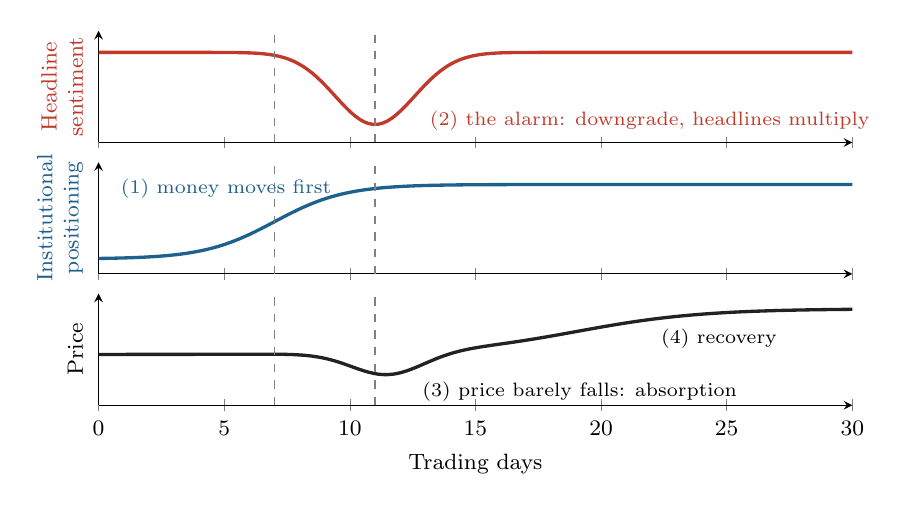
\begin{tikzpicture}
\begin{groupplot}[
  group style={group size=1 by 3, vertical sep=0.25cm, xticklabels at=edge bottom},
  width=0.92\textwidth, height=3.0cm,
  xmin=0, xmax=30, axis lines=left, ytick=\empty,
  xtick={0,5,...,30}, no markers, samples=160, domain=0:30,
  ylabel style={align=center, font=\footnotesize},
  tick label style={font=\footnotesize}, clip=false]
\nextgroupplot[ylabel={\textcolor{echo}{Headline}\\\textcolor{echo}{sentiment}}, ymin=-1.25, ymax=0.3]
  \addplot[echo, very thick] {-exp(-((x-11)^2)/5)};
  \addplot[gray, dashed] coordinates {(7,-1.25) (7,0.3)};
  \addplot[gray, dashed] coordinates {(11,-1.25) (11,0.3)};
  \node[font=\scriptsize, anchor=west, text=echo] at (axis cs:12.8,-0.95) {(2) the alarm: downgrade, headlines multiply};
\nextgroupplot[ylabel={\textcolor{do}{Institutional}\\\textcolor{do}{positioning}}, ymin=-0.2, ymax=1.3]
  \addplot[do, very thick] {1/(1+exp(-(x-7)/1.4))};
  \addplot[gray, dashed] coordinates {(7,-0.2) (7,1.3)};
  \addplot[gray, dashed] coordinates {(11,-0.2) (11,1.3)};
  \node[font=\scriptsize, anchor=west, text=do] at (axis cs:0.5,0.95) {(1) money moves first};
\nextgroupplot[ylabel={Price}, ymin=95, ymax=106, xlabel={\footnotesize Trading days}]
  \addplot[price, very thick] {100 - 2.2*exp(-((x-11.5)^2)/4) + 4.5/(1+exp(-(x-19)/2.5))};
  \addplot[gray, dashed] coordinates {(7,95) (7,106)};
  \addplot[gray, dashed] coordinates {(11,95) (11,106)};
  \node[font=\scriptsize, anchor=west] at (axis cs:12.5,96.3) {(3) price barely falls: absorption};
  \node[font=\scriptsize, anchor=west] at (axis cs:22,101.6) {(4) recovery};
\end{groupplot}
\end{tikzpicture}
\caption{The false-alarm pattern (stylised). Positioning builds (1) before the alarm (2); the price falls far less than the alarm implies (3), then recovers (4). Each step corresponds to a quantity analysed in this paper: lead--lag (\cref{sec:leadlag}), echo (\cref{sec:echo}), absorption (\cref{sec:absorption}).}
\label{fig:pattern}
\end{figure}

Two ideas run through the paper.

\begin{keyidea}[Two ideas]
\textbf{Deeds over words.} When what institutions say and what they do point in different directions, the forecast should lean on what they do. We make this precise twice: the optimal forecast depends on a weighted gap between words and deeds (\cref{thm:saydo}), and the sign of their covariance tells us whether words carry any information at all (\cref{thm:identity}).

\textbf{Fade the echo, follow the news.} A story that merely repeats an earlier one adds no information, so whatever it moves has to come back (\cref{cor:echo}). A genuinely new story that the crowd under-reacts to keeps pushing the price in its direction (\cref{cor:news}).
\end{keyidea}

Neither idea amounts to contrarianism. The same framework tells us to follow the narrative when money confirms it and to fade it only when money, price or timing contradict it (\cref{fig:matrix}).

\begin{figure}[ht]
\centering
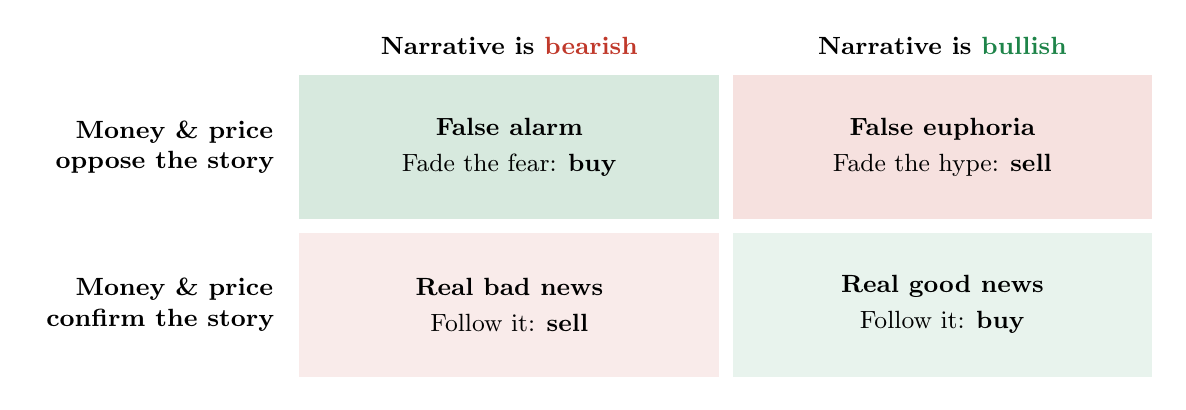
\begin{tikzpicture}[
  cell/.style={draw=white, line width=2pt, minimum width=5.4cm, minimum height=1.9cm, align=center, font=\small},
  head/.style={font=\small\bfseries, align=center}]
\node[cell, fill=good!18] (a) at (0,0) {\textbf{False alarm}\\[2pt] Fade the fear: \textbf{buy}};
\node[cell, fill=echo!15] (b) at (5.5,0) {\textbf{False euphoria}\\[2pt] Fade the hype: \textbf{sell}};
\node[cell, fill=echo!10] (c) at (0,-2.0) {\textbf{Real bad news}\\[2pt] Follow it: \textbf{sell}};
\node[cell, fill=good!10] (d) at (5.5,-2.0) {\textbf{Real good news}\\[2pt] Follow it: \textbf{buy}};
\node[head, above=2pt of a] {Narrative is \textcolor{echo}{bearish}};
\node[head, above=2pt of b] {Narrative is \textcolor{good}{bullish}};
\node[head, left=4pt of a, text width=3.0cm, align=right] {Money \& price\\ \textbf{oppose} the story};
\node[head, left=4pt of c, text width=3.0cm, align=right] {Money \& price\\ \textbf{confirm} the story};
\end{tikzpicture}
\caption{The decision matrix. The narrative alone never determines the trade; its agreement with money and price does.}
\label{fig:matrix}
\end{figure}

\paragraph{What we find.} The main result is a theory of why false alarms happen. We let an informed institution choose both its message and its trade, facing a crowd that partly believes it and a cost of being caught misreporting. The optimal policy is linear in what the institution knows, and it falls into four regimes: telling the truth, shading good news, exaggerating and selling, and, in a thin wedge of parameters, talking the asset down while buying it (\cref{sec:strategic}). Three consequences follow, and we believe each is new.
\begin{itemize}
  \item \emph{Words are switched on and off by one covariance.} The covariance between returns and statements equals price impact times the covariance between trades and statements, minus a noise term. The identity holds for any distribution of value, so the sign of an estimable covariance tells us whether to follow institutional words or fade them (\cref{thm:identity}).
  \item \emph{Virality decides the kind of manipulation.} Media amplification makes the crowd more credulous. In deep, liquid markets this produces false alarms; in thin markets it produces exaggeration, each inside an explicit window of the echo share (\cref{prop:virality}).
  \item \emph{Trust can cycle.} If the crowd re-estimates each period how far to trust institutions, it settles on the truth only when deterrence is strong enough, $\lambda k>1$. Below that threshold credibility alternates between too little and too much, and with weaker deterrence it becomes chaotic (\cref{thm:cycles}).
\end{itemize}

\paragraph{What we measure.} A theory of three voices is useful only if the voices can be measured, and \cref{sec:echo,sec:embeddings,sec:leadlag} build the tools. \emph{Semantic declustering} gives every article an exact probability of being news rather than echo, using both when it appeared and what it says (\cref{thm:semantic}). \emph{Return-aligned embeddings} place stories with similar market consequences close together, and the loss that remains after training certifies which comparisons between stories can be trusted. We give the sharpest certificate of this kind (\cref{thm:racl,thm:robustnn}). Finally, the L\'evy area of positioning against headline tone tells us whether money moved first (\cref{thm:levy}).

\paragraph{What is not new.} Several ingredients are standard, and we flag them where they appear: the Gaussian updating behind \cref{sec:model}, stochastic declustering \citep{zhuang2002}, adaptive conformal inference \citep{gibbs2021} and fractional Kelly sizing. We include them with proofs so that the paper can be read on its own. \Cref{sec:verify} checks every closed form numerically and shows that meaning raises the accuracy of echo attribution from about one in four to $95\%$.

\paragraph{What we test.} \Cref{sec:experiments} puts the tools to work in a simulated market where the truth is known and every quantity has to be estimated. Echoes are separated from news, and fading them pays in every market we simulated. The rolling Say--Do covariance alone separates false-alarm institutions from the rest with an AUC of $0.90$, and a supervised detector built on it reaches $0.93$. Other results are weaker or negative, and we report them as such. Absorption predicts reversal even where the theory allows continuation, because a linear model of the narrative leaves too much of the crowd's reaction behind. The lead--lag signal is weak. The theory's features add almost nothing to a well-fitted linear forecast, although in our simulation even perfect knowledge of value would add little. And the neighbour certificate certifies comparisons only when outcomes are noise-free and the targets sharp.

\paragraph{What we do not claim.} The theory never infers that anyone lied. A ``strategic'' reading means only that words and money moved in opposite directions, in a particular order. Nor does the paper test the theory on market data. That test remains to be done, and \cref{sec:discussion} describes how it should be run.

% =====================================================================
\section{Related Work}\label{sec:related}

\paragraph{Sentiment and returns.} Media pessimism predicts price pressure followed by reversal \citep{tetlock2007}; financial language needs domain-specific measurement \citep{loughran2011}; sentiment matters most where arbitrage is hard \citep{baker2006}. Attention-driven demand \citep{barber2008,da2011} and noise-trader risk \citep{delong1990,shleifer1997} explain persistent mispricing, and heterogeneous-agent models reconcile underreaction with overreaction \citep{hong1999}. Prices drift after headline news and reverse after no-news moves \citep{chan2003}. The same news is interpreted differently across states \citep{veronesi1999}. More broadly, \citet{shiller2017} argues that popular narratives spread like epidemics and drive economic fluctuations. We share the view that narratives move markets, but we model them as \emph{strategic}: the party that shapes a narrative may be trading against it, and its positioning reveals what it believes.

\paragraph{Informed and strategic trading.} Order flow reveals private information \citep{kyle1985,glosten1985}; sophisticated traders exploit predictable flow \citep{brunnermeier2005}; short sellers' edge is superior processing of public news \citep{engelberg2012}; insider trades separate into informative and routine \citep{cohen2012}; promotional articles move prices \citep{kogan2023}. Order-flow imbalance \citep{cont2014} and the square-root impact law \citep{bouchaud2018} quantify the price footprint of trading.

\paragraph{Strategic communication.} Cheap talk \citep{crawford1982}, costly talk with credulous receivers \citep{kartik2007}, market manipulation by informed ``gurus'' with reputational dynamics \citep{benabou1992}, and trading on rumours \citep{vanbommel2003} study how informed agents shape beliefs. Cobweb learning \citep{ezekiel1938,evans2001} and period-doubling in simple maps \citep{may1976} supply the dynamic tools of \cref{sec:strategic}.

\paragraph{Language models in finance.} Supervised text factors \citep{ke2019}, domain encoders \citep{araci2019}, and LLM scores \citep{lopezlira2023} predict returns, subject to look-ahead contamination \citep{glasserman2023}. Our embedding theory builds on contrastive learning \citep{oord2018}, sentence encoders \citep{reimers2019}, and the linear representation hypothesis \citep{park2023}.

\paragraph{Mathematical tools.} Hawkes processes \citep{hawkes1971} admit a cluster representation \citep{hawkesoakes1974} that enables stochastic declustering \citep{zhuang2002}; they are standard in finance \citep{bacry2015}. L\'evy area \citep{levy1940} is the antisymmetric part of the level-two signature \citep{lyons1998,chevyrev2016}. We use Blackwell's garbling order \citep{blackwell1953}, Bhattacharyya bounds \citep{bhattacharyya1943,kailath1967}, adaptive conformal inference \citep{gibbs2021}, and continuous-time growth-optimal portfolios \citep{kelly1956,merton1969}.

% =====================================================================
\section{A Three-Voice Economy}\label{sec:model}

\subsection{Primitives}

\begin{assumption}[Fundamentals and public signals]\label{ass:signals}
The asset's terminal value is $v\sim\N(0,\sigma_v^2)$. A vector of $K$ public channels is observed,
\[
  \y = \h\, v + \bm\nu \in\R^K,\qquad \bm\nu\sim\N(\bm 0,\Sigma_\nu)\ \text{independent of } v,
\]
with $\Sigma_y\coloneqq\sigma_v^2\h\h^\top+\Sigma_\nu\succ0$. Channels are labelled by voice: institutional statements (\SAY), independent news, and media repetition (\ECHO).
\end{assumption}

\begin{assumption}[Price formation]\label{ass:price}
Noise traders submit $u\sim\N(0,\sigma_u^2)$, independent of $(v,\bm\nu)$. Informed traders who know $v$ submit $x=\beta(v-p)$ with $\beta>0$. The price is set by a narrative-sensitive crowd and linear impact:
\[
  p=\bphi^\top\y+\lambda\,(x+u),\qquad \lambda>0,
\]
where $\bphi\in\R^K$ collects the crowd's \emph{narrative multipliers}.
\end{assumption}

\begin{figure}[ht]
\centering
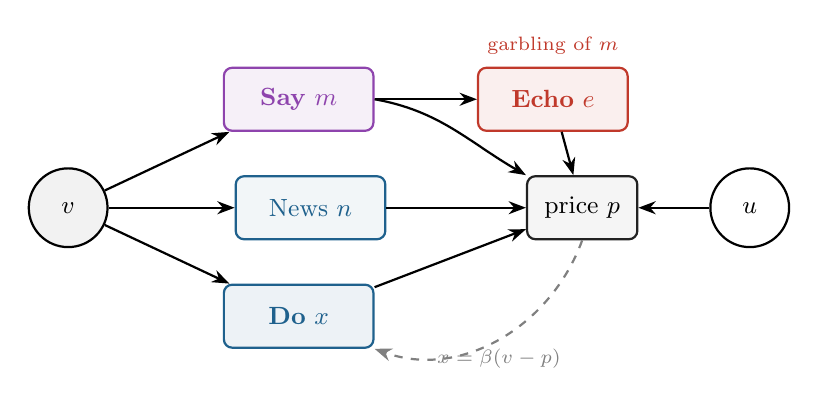
\begin{tikzpicture}[
  node distance=1.0cm and 1.5cm,
  latent/.style={circle, draw, thick, minimum size=1.0cm, font=\small},
  obs/.style={rectangle, rounded corners=3pt, draw, thick, minimum width=1.9cm, minimum height=0.8cm, align=center, font=\small},
  arr/.style={-{Stealth[length=2.2mm]}, thick}]
\node[latent, fill=gray!10] (v) {$v$};
\node[obs, draw=say, fill=say!8, text=say, above right=0.6cm and 1.6cm of v] (m) {\textbf{Say} $m$};
\node[obs, draw=do, fill=do!6, text=do, right=1.6cm of v] (n) {News $n$};
\node[obs, draw=echo, fill=echo!8, text=echo, right=1.3cm of m] (e) {\textbf{Echo} $e$};
\node[obs, draw=do, fill=do!8, text=do, below right=0.6cm and 1.6cm of v] (x) {\textbf{Do} $x$};
\node[obs, draw=price, fill=gray!8, minimum width=1.4cm, right=5.3cm of v] (p) {price $p$};
\node[latent, fill=white, right=0.9cm of p] (u) {$u$};
\draw[arr] (v) -- (m);
\draw[arr] (v) -- (n);
\draw[arr] (m) -- (e);
\draw[arr] (v) -- (x);
\draw[arr] (e) -- (p);
\draw[arr] (n) -- (p);
\draw[arr] (m.east) to[out=-10,in=150] (p.north west);
\draw[arr] (x) -- (p);
\draw[arr] (u) -- (p);
\draw[arr, dashed, gray] (p.south) to[out=-110,in=-20] node[below, font=\scriptsize, text=gray] {$x=\beta(v-p)$} (x.south east);
\node[font=\scriptsize, text=echo, above=1pt of e] {garbling of $m$};
\end{tikzpicture}
\caption{Information structure. The echo channel is a downstream garbling of the institutional statement, while news is an independent signal of $v$. Informed demand reacts to the price (dashed), and the price aggregates every channel.}
\label{fig:dag}
\end{figure}

Throughout, $\kappa\coloneqq(1+\lambda\beta)^{-1}\in(0,1)$, the Bayes weights are $\w^\star\coloneqq\sigma_v^2\Sigma_y^{-1}\h$ (so that $\E[v\mid\y]=\w^{\star\top}\y$), and $\sigma^2_{v|y}\coloneqq\Var(v\mid\y)=\sigma_v^2-\sigma_v^4\h^\top\Sigma_y^{-1}\h$. The forward return is $r\coloneqq v-p$.

\begin{lemma}[Price and return]\label{lem:price}
Under \cref{ass:signals,ass:price},
\[
  p=\kappa\big(\bphi^\top\y+\lambda\beta v+\lambda u\big),\qquad r=\kappa\big(v-\bphi^\top\y-\lambda u\big).
\]
\end{lemma}
\begin{proof}
Substituting $x=\beta(v-p)$ gives $p(1+\lambda\beta)=\bphi^\top\y+\lambda\beta v+\lambda u$. Then $r=v-p=\kappa\big((1+\lambda\beta)v-\bphi^\top\y-\lambda\beta v-\lambda u\big)=\kappa(v-\bphi^\top\y-\lambda u)$.
\end{proof}

\subsection{Follow or fade}

\begin{theorem}[Follow-or-fade]\label{thm:followfade}
Under \cref{ass:signals,ass:price},
\[
  \E[r\mid\y]=\kappa\,(\w^\star-\bphi)^\top\y,\qquad \Var(r\mid\y)=\kappa^2\big(\sigma^2_{v|y}+\lambda^2\sigma_u^2\big)\eqqcolon\varsigma^2 .
\]
The predictive loading on channel $k$ is negative (\emph{fade}) if and only if $\varphi_k>w^\star_k$, and positive (\emph{follow}) if and only if $\varphi_k<w^\star_k$.
\end{theorem}
\begin{proof}
By \cref{lem:price}, $r=\kappa(v-\bphi^\top\y-\lambda u)$. Joint Gaussianity gives $\E[v\mid\y]=\Cov(v,\y)\Sigma_y^{-1}\y=\sigma_v^2\h^\top\Sigma_y^{-1}\y=\w^{\star\top}\y$, and $\E[u\mid\y]=0$ by independence. For the variance, $r-\E[r\mid\y]=\kappa\big((v-\E[v\mid\y])-\lambda u\big)$, and the two terms are independent given $\y$.
\end{proof}

\begin{figure}[ht]
\centering
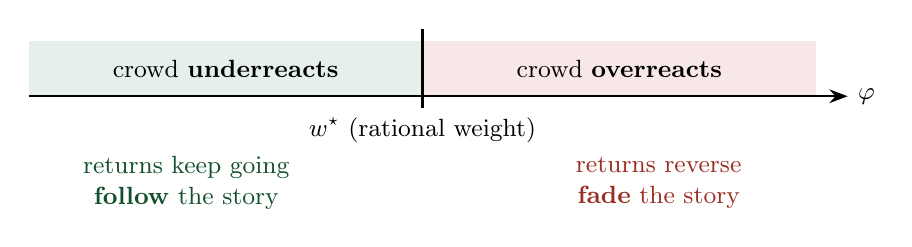
\begin{tikzpicture}[font=\small]
\fill[good!12] (0,0) rectangle (5,0.7);
\fill[echo!12] (5,0) rectangle (10,0.7);
\draw[thick,-{Stealth}] (0,0) -- (10.4,0) node[right] {$\varphi$};
\draw[very thick] (5,-0.15) -- (5,0.85);
\node[below] at (5,-0.15) {$w^\star$ (rational weight)};
\node[align=center] at (2.5,0.35) {crowd \textbf{underreacts}};
\node[align=center] at (7.5,0.35) {crowd \textbf{overreacts}};
\node[align=center, text=good!60!black] at (2.0,-1.1) {returns keep going\\ \textbf{follow} the story};
\node[align=center, text=echo!80!black] at (8.0,-1.1) {returns reverse\\ \textbf{fade} the story};
\end{tikzpicture}
\caption{\Cref{thm:followfade} for a single channel: the sign of return predictability is set by the crowd's multiplier relative to the Bayes weight.}
\label{fig:phi}
\end{figure}

\begin{corollary}[Fade the echo]\label{cor:echo}
Suppose channel $e$ is a garbling of the other channels: $e=\bm a^\top\y_{-e}+\xi$ with $\xi\sim\N(0,\sigma_\xi^2)$, $\sigma_\xi^2>0$, independent of $(v,\y_{-e},u)$. Then $w^\star_e=0$, and the predictive loading on $e$ equals $-\kappa\varphi_e$. Any positive crowd weight on echo is therefore predictably reversed.
\end{corollary}
\begin{proof}
$\sigma(\y)=\sigma(\y_{-e},\xi)$ and $\xi$ is independent of $(v,\y_{-e})$, so $\E[v\mid\y]=\E[v\mid\y_{-e}]$, a linear function of $\y_{-e}$ alone. If $\E[v\mid\y]=\w^{\star\top}\y=\w'^{\top}\y$ with $w'_e=0$, then $(\w^\star-\w')^\top\y=0$ almost surely, so $(\w^\star-\w')^\top\Sigma_y(\w^\star-\w')=0$, and $\Sigma_y\succ0$ forces $\w^\star=\w'$. Hence $w^\star_e=0$, and \cref{thm:followfade} gives the loading $\kappa(0-\varphi_e)$.
\end{proof}

\begin{corollary}[Follow the news]\label{cor:news}
Suppose channel $n=v+\nu_n$ with $\nu_n\sim\N(0,\sigma_n^2)$ independent of $(v,\y_{-n},u)$, and let $s^2\coloneqq\Var(v\mid\y_{-n})>0$. Then $w^\star_n=s^2/(s^2+\sigma_n^2)\in(0,1)$, and returns drift in the direction of $n$ whenever the crowd underweights it, $\varphi_n<w^\star_n$.
\end{corollary}
\begin{proof}
Conditionally on $\y_{-n}$, $v\sim\N(\mu',s^2)$ with $\mu'$ linear in $\y_{-n}$, and $n=v+\nu_n$. The scalar Gaussian update gives $\E[v\mid\y]=\mu'+\frac{s^2}{s^2+\sigma_n^2}(n-\mu')$, whose coefficient on $n$ is $w^\star_n$. Apply \cref{thm:followfade}.
\end{proof}

\begin{intuition}
Repetition adds attention but no information, so whatever price effect it has must unwind. Genuinely new information that the crowd underweights keeps moving the price. This is the formal content of ``fade the echo, follow the news''.
\end{intuition}

\subsection{Deeds over words}

\begin{theorem}[Say--Do gap optimality]\label{thm:saydo}
In addition to $\y$, the econometrician observes a positioning proxy $\hat x=x+\xi_x$, $\xi_x\sim\N(0,\sigma_x^2)$ independent of $(v,\bm\nu,u)$. Let
\[
  c_x\coloneqq\frac{\beta\varsigma^2}{\beta^2\varsigma^2+\sigma_x^2},\qquad \theta\coloneqq\frac{\sigma_x^2}{\beta^2\varsigma^2+\sigma_x^2}\in(0,1].
\]
Then
\begin{enumerate}[label=(\roman*)]
  \item $\E[r\mid\y,\hat x]=\theta\,\kappa(\w^\star-\bphi)^\top\y+c_x\,\hat x$ and $\Var(r\mid\y,\hat x)=\theta\,\varsigma^2<\varsigma^2$ whenever $\sigma_x^2<\infty$;
  \item if the \SAY\ channel $m=y_1$ is overweighted, $\varphi_1>w^\star_1$, the forecast depends on $(m,\hat x)$ only through the \emph{Say--Do gap}
  \[
    G_\gamma\coloneqq\gamma\, m-\hat x,\qquad \gamma\coloneqq\frac{\theta\kappa(\varphi_1-w^\star_1)}{c_x}>0,
  \]
  entering with coefficient $-c_x<0$.
\end{enumerate}
\end{theorem}
\begin{proof}
By \cref{lem:price}, $x=\beta(v-p)=\beta r$, so $\hat x=\beta r+\xi_x$. Conditionally on $\y$, $(r,\hat x)$ is Gaussian with $\Cov(r,\hat x\mid\y)=\beta\varsigma^2$, $\Var(\hat x\mid\y)=\beta^2\varsigma^2+\sigma_x^2$ and $\E[\hat x\mid\y]=\beta\E[r\mid\y]$. Gaussian conditioning (\cref{lem:gauss}) gives
\[
  \E[r\mid\y,\hat x]=\E[r\mid\y]+c_x\big(\hat x-\beta\E[r\mid\y]\big)=(1-\beta c_x)\E[r\mid\y]+c_x\hat x,
\]
with $1-\beta c_x=\theta$, and $\Var(r\mid\y,\hat x)=\varsigma^2-c_x\beta\varsigma^2=\theta\varsigma^2$. For (ii), the terms in $m$ and $\hat x$ are $-\theta\kappa(\varphi_1-w^\star_1)m+c_x\hat x=-c_x(\gamma m-\hat x)$.
\end{proof}

\begin{figure}[ht]
\centering
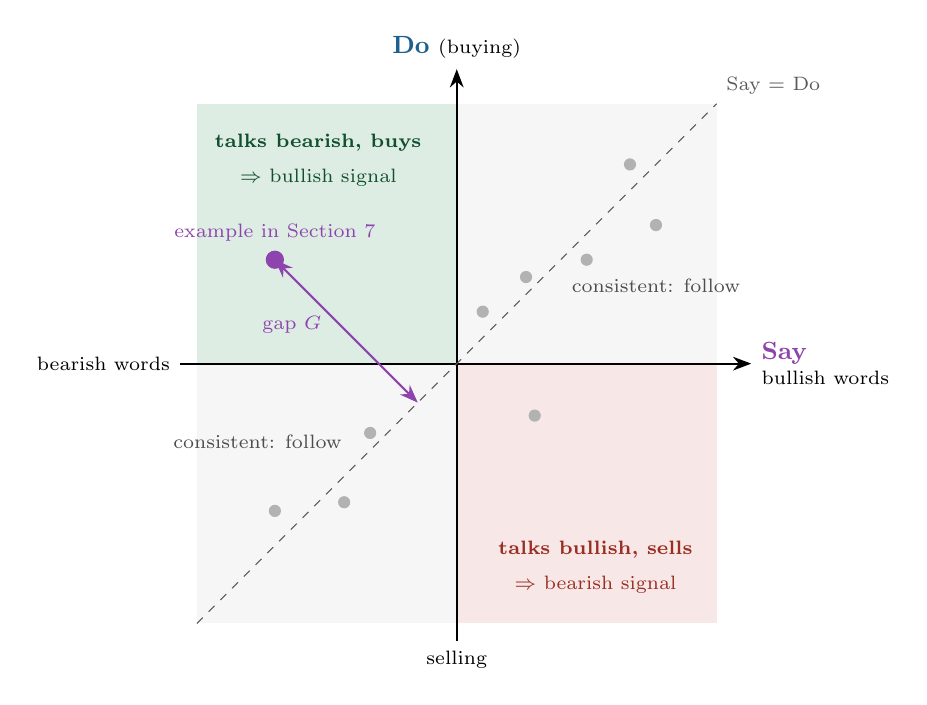
\begin{tikzpicture}[scale=1.1]
\fill[good!15] (-3,0) rectangle (0,3);
\fill[echo!12] (0,-3) rectangle (3,0);
\fill[gray!7] (0,0) rectangle (3,3);
\fill[gray!7] (-3,-3) rectangle (0,0);
\draw[-{Stealth}, thick] (-3.2,0) -- (3.4,0) node[right, font=\small, align=left] {\SAY\\[-2pt]\scriptsize bullish words};
\draw[-{Stealth}, thick] (0,-3.2) -- (0,3.4) node[above, font=\small, align=center] {\DO\ \scriptsize (buying)};
\node[font=\scriptsize, anchor=east] at (-3.2,0) {bearish words};
\node[font=\scriptsize, anchor=north] at (0,-3.2) {selling};
\draw[dashed, gray!70!black] (-3,-3) -- (3,3) node[above right, font=\scriptsize, text=gray!70!black] {Say = Do};
\node[font=\scriptsize\bfseries, text=good!60!black, align=center] at (-1.6,2.55) {talks bearish, buys};
\node[font=\scriptsize, text=good!60!black, align=center] at (-1.6,2.15) {$\Rightarrow$ bullish signal};
\node[font=\scriptsize\bfseries, text=echo!80!black, align=center] at (1.6,-2.15) {talks bullish, sells};
\node[font=\scriptsize, text=echo!80!black, align=center] at (1.6,-2.55) {$\Rightarrow$ bearish signal};
\node[font=\scriptsize, text=gray!60!black, align=center] at (2.3,0.9) {consistent: follow};
\node[font=\scriptsize, text=gray!60!black, align=center] at (-2.3,-0.9) {consistent: follow};
\foreach \p in {(0.8,1.0),(1.5,1.2),(2.0,2.3),(-1.0,-0.8),(-2.1,-1.7),(0.3,0.6),(-1.3,-1.6),(2.3,1.6),(0.9,-0.6)}
  \fill[gray!60] \p circle (2pt);
\fill[say] (-2.1,1.2) circle (3pt);
\node[font=\scriptsize, text=say, anchor=south] at (-2.1,1.3) {example in Section 7};
\draw[{Stealth}-{Stealth}, say, thick] (-2.1,1.2) -- (-0.45,-0.45);
\node[font=\scriptsize, text=say, anchor=east] at (-1.45,0.45) {gap $G$};
\end{tikzpicture}
\caption{The Say--Do plane. \Cref{thm:saydo} shows that the optimal forecast is a decreasing function of the signed distance from the line $\hat x=\gamma m$. Top-left is the false-alarm zone; bottom-right is the false-euphoria zone.}
\label{fig:saydo}
\end{figure}

\subsection{Absorption: informed or noise?}\label{sec:absorption}

The \emph{absorption} of a narrative shock is the price move net of the narrative-implied move, $a\coloneqq p-\bphi^\top\y$.

\begin{theorem}[Absorption sign]\label{thm:absorption}
Under \cref{ass:signals,ass:price},
\[
  \E[r\mid\y,a]=\E[r\mid\y]+c_A\big(a-\E[a\mid\y]\big),\qquad
  c_A=\frac{\beta\,\sigma^2_{v|y}-\lambda\,\sigma_u^2}{\lambda\,\big(\beta^2\sigma^2_{v|y}+\sigma_u^2\big)} .
\]
Absorption therefore predicts \emph{continuation} in its own direction if and only if $\beta\sigma^2_{v|y}>\lambda\sigma_u^2$, and \emph{reversal} if and only if $\beta\sigma^2_{v|y}<\lambda\sigma_u^2$. In the limits, $c_A=1/(\lambda\beta)$ when $\sigma_u=0$ (absorption is sufficient for $r$) and $c_A=-1$ when $\beta=0$ (pure noise fully reverts).
\end{theorem}
\begin{proof}
Write $\tilde v\coloneqq v-\E[v\mid\y]$, independent of $u$ given $\y$. By \cref{lem:price}, $r-\E[r\mid\y]=\kappa(\tilde v-\lambda u)$. Since $a=\lambda(x+u)=\lambda\beta r+\lambda u$,
\[
  a-\E[a\mid\y]=\lambda\beta\kappa(\tilde v-\lambda u)+\lambda u=\lambda\beta\kappa\,\tilde v+\lambda(1-\lambda\beta\kappa)u=\lambda\kappa(\beta\tilde v+u),
\]
using $1-\lambda\beta\kappa=\kappa$. Hence $\Cov(r,a\mid\y)=\lambda\kappa^2(\beta\sigma^2_{v|y}-\lambda\sigma_u^2)$ and $\Var(a\mid\y)=\lambda^2\kappa^2(\beta^2\sigma^2_{v|y}+\sigma_u^2)$, and \cref{lem:gauss} gives $c_A$ as their ratio. The limits follow by substitution.
\end{proof}

\begin{lemma}[Robustness to a misspecified multiplier]\label{lem:robust}
For any $\hat\bphi\in\R^K$, let $\hat a\coloneqq p-\hat\bphi^\top\y$. Then $\sigma(\y,\hat a)=\sigma(\y,a)$ and hence $\E[r\mid\y,\hat a]=\E[r\mid\y,a]$.
\end{lemma}
\begin{proof}
$\hat a=a+(\bphi-\hat\bphi)^\top\y$ is an invertible affine function of $a$ given $\y$, and conversely.
\end{proof}

\begin{remark}[Kyle calibration]
Plugging in the single-period equilibrium intensities of \citet{kyle1985}, $\beta=\sigma_u/\sigma_{v|y}$ and $\lambda=\sigma_{v|y}/(2\sigma_u)$, gives $\beta\sigma^2_{v|y}=\sigma_u\sigma_{v|y}>\tfrac12\sigma_u\sigma_{v|y}=\lambda\sigma_u^2$ and $c_A=\tfrac12$: absorption is informative and predicts continuation.
\end{remark}

\begin{remark}[Relation to volume--return dynamics]
\Cref{thm:absorption} is in the spirit of \citet{llorente2002}, where high-volume returns continue when informed trading dominates and reverse when hedging dominates. The difference is that we condition on the \emph{narrative}: the object is the price move net of what the public story implied. By \cref{lem:robust}, its information content survives misestimation of the crowd's multiplier.
\end{remark}

\begin{figure}[ht]
\centering
\begin{minipage}{0.5\textwidth}
\centering
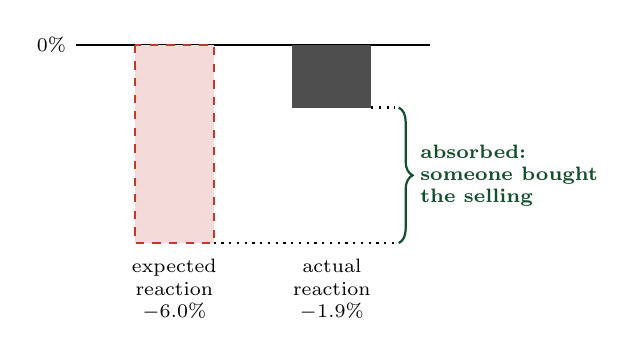
\begin{tikzpicture}[xscale=0.5, yscale=0.42, font=\small]
\draw[thick] (-0.5,0) -- (8.5,0);
\node[anchor=east, font=\scriptsize] at (-0.5,0) {0\%};
\fill[echo!18] (1,0) rectangle (3,-6);
\draw[echo, thick, dashed] (1,0) rectangle (3,-6);
\node[font=\scriptsize, align=center, anchor=north] at (2,-6.2) {expected\\ reaction\\ $-6.0\%$};
\fill[price!80] (5,0) rectangle (7,-1.9);
\node[font=\scriptsize, align=center, anchor=north] at (6,-6.2) {actual\\ reaction\\ $-1.9\%$};
\draw[dotted, thick] (3,-6) -- (7.6,-6);
\draw[dotted, thick] (7,-1.9) -- (7.6,-1.9);
\draw[decorate, decoration={brace, amplitude=5pt, mirror}, thick, good!60!black] (7.7,-6) -- (7.7,-1.9);
\node[font=\scriptsize\bfseries, text=good!60!black, anchor=west, align=left] at (8.0,-3.95) {absorbed:\\ someone bought\\ the selling};
\end{tikzpicture}
\end{minipage}\hfill
\begin{minipage}{0.45\textwidth}
\centering
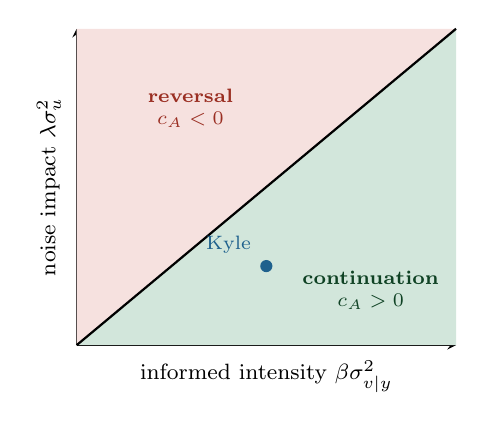
\begin{tikzpicture}
\begin{axis}[width=6.4cm, height=5.6cm, xmin=0, xmax=2, ymin=0, ymax=2,
  xlabel={\footnotesize informed intensity $\beta\sigma^2_{v|y}$},
  ylabel={\footnotesize noise impact $\lambda\sigma_u^2$},
  xtick=\empty, ytick=\empty, axis lines=left, clip=false]
\addplot[name path=diag, thick, black, domain=0:2] {x};
\addplot[name path=bottom, draw=none, domain=0:2] {0};
\addplot[name path=top, draw=none, domain=0:2] {2};
\addplot[good!20] fill between[of=diag and bottom];
\addplot[echo!15] fill between[of=top and diag];
\node[font=\scriptsize\bfseries, text=good!50!black, align=center] at (axis cs:1.55,0.35) {continuation\\ $c_A>0$};
\node[font=\scriptsize\bfseries, text=echo!80!black, align=center] at (axis cs:0.6,1.5) {reversal\\ $c_A<0$};
\fill[do] (axis cs:1,0.5) circle (2.2pt);
\node[font=\scriptsize, text=do, anchor=south east] at (axis cs:0.97,0.52) {Kyle};
\end{axis}
\end{tikzpicture}
\end{minipage}
\caption{Left: absorption as the gap between the narrative-implied and actual reaction. Right: phase diagram of \cref{thm:absorption}. Absorption signals a hidden buyer only below the diagonal, where informed flow dominates noise.}
\label{fig:absorb}
\end{figure}

% =====================================================================
\section{Strategic Speech: An Endogenous Theory of False Alarms}\label{sec:strategic}

So far the \SAY\ channel has been exogenous. We now let the institution \emph{choose} what to say while it trades, facing a crowd that partially believes it. The literature on cheap talk \citep{crawford1982}, costly talk with credulous receivers \citep{kartik2007}, insider and ``guru'' manipulation \citep{benabou1992} and rumour-based trading \citep{vanbommel2003} establishes that such incentives exist. Our model is deliberately linear--quadratic, so that every object has a closed form, and it is coupled to the echo and positioning measurements of this paper. It delivers four results that are, to our knowledge, new: a complete taxonomy of optimal speech with an explicit false-alarm region (\cref{thm:speech,cor:taxonomy}); a distribution-free identity linking the predictive content of words to the covariance between words and deeds (\cref{thm:identity}); a dichotomy for how media virality produces manipulation (\cref{prop:virality}); and a period-doubling route to \emph{credibility cycles} under adaptive trust (\cref{thm:cycles}).

\begin{assumption}[Strategic institution]\label{ass:strategic}
An institution knows $v$, which has an arbitrary distribution with mean zero and variance $\sigma_v^2<\infty$. It publishes a message $m$ and trades $x$. The public observes $\tilde m=m+\varepsilon$, where $\varepsilon$ has mean zero and variance $\sigma_\varepsilon^2$ and is independent of $v$. The price is $p=\varphi\tilde m+\lambda x$, where $\varphi\ge0$ is the crowd's effective credulity and $\lambda>0$ is price impact. Misreporting costs $\tfrac k2(m-v)^2$ with $k>0$ (legal, reputational). The institution maximises
\[
  J(x,m)=\E\big[x(v-p)\mid v\big]-\tfrac k2(m-v)^2=x(v-\varphi m-\lambda x)-\tfrac k2(m-v)^2 .
\]
We write $a\coloneqq2\lambda k$ for the \emph{deterrence--impact product}.
\end{assumption}

\begin{assumption}[Echo amplification]\label{ass:amplify}
Each article moves the price by $\varphi_0$ per unit of message, and the message propagates through a Hawkes cascade with branching ratio $n\in[0,1)$. By \cref{prop:branching}, the expected cascade size is $(1-n)^{-1}$, so the effective credulity is $\varphi=\varphi_0/(1-n)$.
\end{assumption}

\subsection{Optimal speech and its taxonomy}

\begin{theorem}[Optimal speech and trade]\label{thm:speech}
Under \cref{ass:strategic}, $J$ has a unique maximiser if and only if $a>\varphi^2$, in which case
\[
  m^\ast=\psi\,v,\qquad x^\ast=\chi\,v,\qquad
  \psi=\frac{a-\varphi}{a-\varphi^2},\qquad \chi=\frac{k(1-\varphi)}{a-\varphi^2}.
\]
If $a<\varphi^2$, $J$ is unbounded above: manipulation is limited only by position constraints.
\end{theorem}
\begin{proof}
$J$ is quadratic in $(x,m)$ with Hessian $H=\begin{psmallmatrix}-2\lambda&-\varphi\\-\varphi&-k\end{psmallmatrix}$. Since $-2\lambda<0$, $H$ is negative definite iff $\det H=a-\varphi^2>0$. In that case $J$ is strictly concave and its unique maximiser solves the first-order conditions $v-\varphi m-2\lambda x=0$ and $-\varphi x-k(m-v)=0$. Substituting $x=(v-\varphi m)/(2\lambda)$ into the second condition gives $m(a-\varphi^2)=v(a-\varphi)$. Then $x=(1-\varphi\psi)v/(2\lambda)$, and $1-\varphi\psi=a(1-\varphi)/(a-\varphi^2)$ gives $\chi$. If $\det H<0$, $H$ has a positive eigenvalue with eigenvector $\bm d$, and $J(t\bm d)\to\infty$ as $t\to\infty$.
\end{proof}

\begin{corollary}[Taxonomy of speech]\label{cor:taxonomy}
Let $a>\varphi^2$ and $v>0$.
\begin{enumerate}[label=(\roman*)]
  \item \textbf{Truth} ($\varphi=1$): $\psi=1$, $\chi=0$.
  \item \textbf{Shading} ($\varphi<1$, $a>\varphi$): $0<\psi<1$ and $\chi>0$. The institution understates good news and buys.
  \item \textbf{False alarm} ($\varphi<1$, $\varphi^2<a<\varphi$): $\psi<0<\chi$. The institution talks the asset \emph{down} while buying it.
  \item \textbf{Exaggeration and distribution} ($\varphi>1$): $\psi>1$ and $\chi<0$. The institution overstates and sells into the hype.
\end{enumerate}
\end{corollary}
\begin{proof}
$\psi>0\iff a>\varphi$ (the denominator is positive); $\psi<1\iff\varphi^2<\varphi\iff\varphi<1$; and $\sgn\chi=\sgn(1-\varphi)$. When $\varphi>1$, $a>\varphi^2>\varphi$, so $\psi>1$.
\end{proof}

\begin{figure}[ht]
\centering
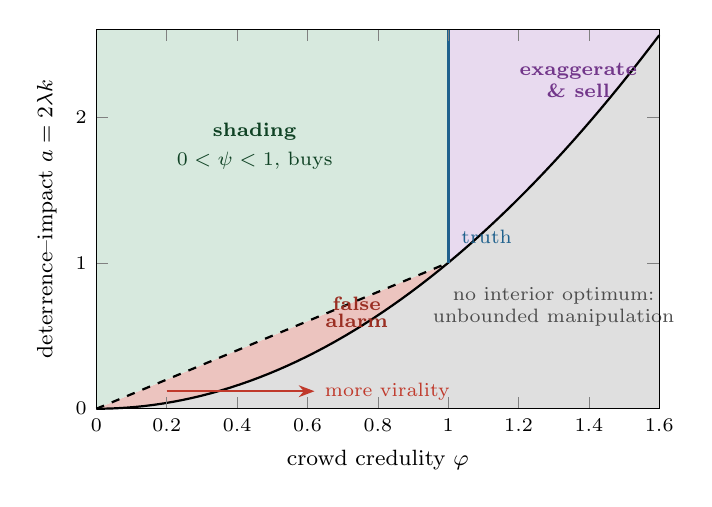
\begin{tikzpicture}
\begin{axis}[width=0.72\textwidth, height=6.4cm, xmin=0, xmax=1.6, ymin=0, ymax=2.6,
  xlabel={\footnotesize crowd credulity $\varphi$},
  ylabel={\footnotesize deterrence--impact $a=2\lambda k$},
  tick label style={font=\scriptsize}, axis on top, clip=false]
\addplot[name path=sq, draw=black, thick, domain=0:1.6, samples=60] {x^2};
\addplot[name path=lin, draw=black, thick, dashed, domain=0:1, samples=2] {x};
\addplot[name path=top, draw=none, domain=0:1.6, samples=2] {2.6};
\addplot[name path=bot, draw=none, domain=0:1.6, samples=2] {0};
\addplot[gray!25] fill between[of=sq and bot];
\addplot[echo!30] fill between[of=lin and sq, soft clip={domain=0:1}];
\addplot[good!18] fill between[of=top and lin, soft clip={domain=0:1}];
\addplot[say!20] fill between[of=top and sq, soft clip={domain=1:1.6}];
\draw[do, very thick] (axis cs:1,1) -- (axis cs:1,2.6);
\node[font=\scriptsize\bfseries, text=good!50!black] at (axis cs:0.45,1.9) {shading};
\node[font=\scriptsize, text=good!50!black] at (axis cs:0.45,1.7) {$0<\psi<1$, buys};
\node[font=\scriptsize\bfseries, text=echo!80!black, align=center] at (axis cs:0.74,0.66) {false\\[-2pt] alarm};
\node[font=\scriptsize\bfseries, text=say!80!black, align=center] at (axis cs:1.37,2.25) {exaggerate\\ \& sell};
\node[font=\scriptsize, text=gray!60!black, align=center] at (axis cs:1.3,0.7) {no interior optimum:\\ unbounded manipulation};
\node[font=\scriptsize, text=do, anchor=west, align=left] at (axis cs:1.01,1.18) {truth};
\draw[-{Stealth[length=2mm]}, thick, echo] (axis cs:0.2,0.12) -- (axis cs:0.62,0.12) node[right, font=\scriptsize] {more virality};
\end{axis}
\end{tikzpicture}
\caption{Regime map of \cref{thm:speech,cor:taxonomy}. Echo amplification moves the market to the right ($\varphi=\varphi_0/(1-n)$). False alarms, which talk down an asset while buying it, occupy the thin red wedge between $a=\varphi^2$ and $a=\varphi$.}
\label{fig:regimemap}
\end{figure}

\subsection{Words, deeds and returns}

\begin{theorem}[Say--Do covariance identity]\label{thm:identity}
Under \cref{ass:strategic}, let the message rule $m=m(v)$ be \emph{arbitrary} (measurable, square-integrable) and let the trade be optimal given the message. Then the forward return $r\coloneqq v-p$ satisfies, pathwise,
\[
  r=\lambda x-\varphi\varepsilon,
\]
and therefore, for any distribution of $v$,
\[
  \Cov(r,\tilde m)=\lambda\,\Cov(x,\tilde m)-\varphi\,\sigma_\varepsilon^2,\qquad \E[r\mid x]=\lambda x .
\]
In particular, whenever \SAY\ and \DO\ covary negatively, returns load negatively on \SAY: words are to be faded. In the equilibrium of \cref{thm:speech}, $\Cov(x,\tilde m)=\psi\chi\,\sigma_v^2$, which is negative exactly in the false-alarm and exaggeration regimes.
\end{theorem}
\begin{proof}
Given $m$, the trade maximises $x(v-\varphi m-\lambda x)$, so $x=(v-\varphi m)/(2\lambda)$, that is, $v-\varphi m=2\lambda x$. Hence $r=v-\varphi(m+\varepsilon)-\lambda x=2\lambda x-\lambda x-\varphi\varepsilon$. Since $x$ and $m$ are functions of $v$, which is independent of $\varepsilon$, we have $\Cov(\varepsilon,\tilde m)=\sigma_\varepsilon^2$, and $\E[\varepsilon\mid x]=0$. The equilibrium covariance is $\Cov(\chi v,\psi v)$, and $\psi\chi<0$ exactly in regimes (iii) and (iv) of \cref{cor:taxonomy}.
\end{proof}

\begin{keyidea}[Why the identity matters]
The identity requires no distributional assumption, and both sides are estimable. The rolling sign of $\widehat{\Cov}(\text{Say},\text{Do})$ tells the econometrician whether to follow or fade institutional words. Deeds are always followed, with slope equal to price impact. \Cref{thm:identity} is the strategic counterpart of \cref{thm:saydo}: there the Say--Do gap was the optimal forecast direction; here the Say--Do \emph{covariance} is the switch that sets its sign.
\end{keyidea}

\subsection{Virality and the manipulation dichotomy}

\begin{proposition}[Manipulation dichotomy]\label{prop:virality}
Under \cref{ass:strategic,ass:amplify} with $\varphi_0\in(0,1)$, call a regime \emph{manipulative} if $\Cov(\text{Say},\text{Do})<0$.
\begin{enumerate}[label=(\roman*)]
  \item If $a<1$, the only reachable manipulative regime is the false alarm. It occurs if and only if
  $\max\{0,\,1-\varphi_0/a\}<n<1-\varphi_0/\sqrt a$.
  \item If $a>1$, the only reachable manipulative regime is exaggeration. It occurs if and only if $1-\varphi_0<n<1-\varphi_0/\sqrt a$.
  \item If $n>1-\varphi_0/\sqrt a$, no interior optimum exists.
\end{enumerate}
\end{proposition}
\begin{proof}
$\varphi=\varphi_0/(1-n)$ increases continuously from $\varphi_0$ to $\infty$ on $[0,1)$. The false alarm requires $\varphi^2<a<\varphi<1$, hence $a<1$. Exaggeration requires $1<\varphi<\sqrt a$, hence $a>1$. The two are therefore mutually exclusive. The conditions $\varphi>a$, $\varphi>1$ and $\varphi<\sqrt a$ are equivalent to $n>1-\varphi_0/a$, $n>1-\varphi_0$ and $n<1-\varphi_0/\sqrt a$ respectively. For $a<1$ we have $\sqrt a<1$, so $\varphi<\sqrt a$ already implies $\varphi<1$. Part (iii) is \cref{thm:speech}.
\end{proof}

\begin{figure}[ht]
\centering
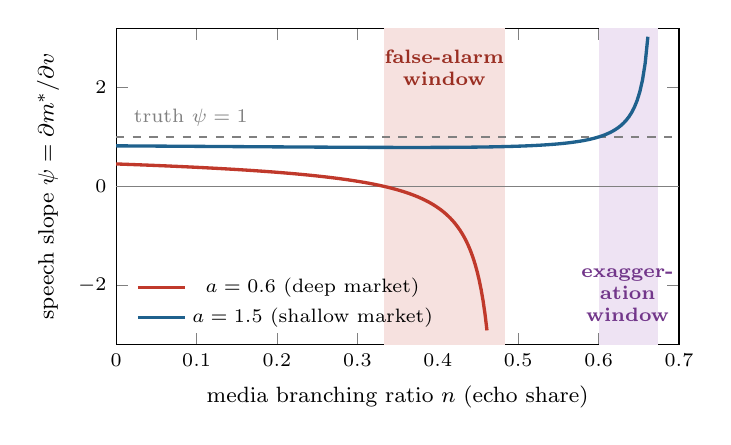
\begin{tikzpicture}
\begin{axis}[width=0.72\textwidth, height=5.6cm, xmin=0, xmax=0.7, ymin=-3.2, ymax=3.2,
  xlabel={\footnotesize media branching ratio $n$ (echo share)},
  ylabel={\footnotesize speech slope $\psi=\partial m^\ast/\partial v$},
  tick label style={font=\scriptsize}, unbounded coords=jump,
  legend style={font=\scriptsize, draw=none, fill=none, at={(0.02,0.02)}, anchor=south west}]
\fill[echo!15] (axis cs:0.3333,-3.2) rectangle (axis cs:0.4836,3.2);
\fill[say!15] (axis cs:0.6,-3.2) rectangle (axis cs:0.6734,3.2);
\addplot[gray, thin, forget plot] coordinates {(0,0) (0.7,0)};
\addplot[gray, thin, dashed, forget plot] coordinates {(0,1) (0.7,1)};
\addplot[echo, very thick, domain=0:0.478, samples=200, restrict y to domain=-3.3:3.3]
  {(0.6-0.4/(1-x))/(0.6-(0.4/(1-x))^2)};
\addlegendentry{$a=0.6$ (deep market)}
\addplot[do, very thick, domain=0:0.668, samples=200, restrict y to domain=-3.3:3.3]
  {(1.5-0.4/(1-x))/(1.5-(0.4/(1-x))^2)};
\addlegendentry{$a=1.5$ (shallow market)}
\node[font=\scriptsize\bfseries, text=echo!80!black, align=center] at (axis cs:0.408,2.4) {false-alarm\\ window};
\node[font=\scriptsize\bfseries, text=say!80!black, align=center] at (axis cs:0.636,-2.2) {exagger-\\ ation\\ window};
\node[font=\scriptsize, text=gray, anchor=south west] at (axis cs:0.01,1.02) {truth $\psi=1$};
\end{axis}
\end{tikzpicture}
\caption{\Cref{prop:virality} with $\varphi_0=0.4$. As the echo share rises, a deep market (small $a$) passes through a false-alarm window where the speech slope turns negative. A shallow market (large $a$) instead passes through an exaggeration window with $\psi>1$. Both windows end where no interior optimum exists.}
\label{fig:virality}
\end{figure}

\subsection{Adaptive trust and credibility cycles}

Suppose that after each round the crowd resets its credulity to the least-squares slope of value on message under the previous round's strategy, a cobweb-type learning rule \citep{ezekiel1938,evans2001}. With noiseless messages $m_t=\psi(\varphi_t)v$, this gives
\[
  \varphi_{t+1}=\frac{\Cov(v,m_t)}{\Var(m_t)}=\frac{1}{\psi(\varphi_t)}=F_a(\varphi_t),\qquad F_a(\varphi)\coloneqq\frac{a-\varphi^2}{a-\varphi},
\]
on the admissible set $\mathcal{D}_a=\{\varphi:\varphi^2<a,\ \varphi\neq a,\ \psi(\varphi)\neq0\}$.

\begin{theorem}[Credibility cycles]\label{thm:cycles}
Let $a=2\lambda k$.
\begin{enumerate}[label=(\roman*)]
  \item For $a>1$, the truthful state $\varphi=1$ is the unique fixed point of $F_a$ in $\mathcal{D}_a$. For $a\le1$ there is no admissible fixed point.
  \item $F_a'(1)=-1/(a-1)$. The truthful state is locally asymptotically stable if and only if $a>2$, that is, $\lambda k>1$. For $1<a<2$ it is repelling, and orbits leave it with alternating overshoots.
  \item For $1<a<2$, $F_a$ has exactly one $2$-cycle,
  \[
    \varphi_\pm=\frac{a\pm\sqrt{a(2-a)}}{2},\qquad \varphi_-<1<\varphi_+,\qquad \varphi_\pm\in\mathcal{D}_a,
  \]
  with multiplier $(F_a^{2})'(\varphi_\pm)=(5a-9)/(a-1)$. It is locally asymptotically stable if and only if $\tfrac53<a<2$, that is, $\tfrac56<\lambda k<1$. Along the cycle the market alternates between shading (under-trust, $\varphi_-$) and exaggeration (over-trust, $\varphi_+$), so the sign of $\Cov(\text{Say},\text{Do})$ alternates from round to round.
  \item The cycle is born from the truthful state at $a=2$, where $\varphi_\pm\to1$ and the multiplier equals $1$ (a flip bifurcation). It loses stability at $a=\tfrac53$, where the multiplier equals $-1$ (a second flip).
\end{enumerate}
\end{theorem}
\begin{proof}
(i) $F_a(\varphi)=\varphi\iff a-\varphi^2=a\varphi-\varphi^2\iff\varphi=1$. Admissibility of $\varphi=1$ requires $1<a$.
(ii) $F_a'(\varphi)=(a-2a\varphi+\varphi^2)/(a-\varphi)^2$, so $F_a'(1)=(1-a)/(a-1)^2=-1/(a-1)$, and $|F_a'(1)|<1\iff a>2$.
(iii) Using $a-F_a(\varphi)=(a^2-a\varphi-a+\varphi^2)/(a-\varphi)$, a direct computation gives
\[
  F_a(F_a(\varphi))-\varphi=\frac{-a(\varphi-1)\big(2\varphi^2-2a\varphi+a^2-a\big)}{(a-\varphi)^2\,\big(a-F_a(\varphi)\big)} .
\]
The quadratic factor has roots $\varphi_\pm$, which are real and distinct from $1$ for $1<a<2$ (at $\varphi=1$ it equals $(a-1)(a-2)\neq0$). They are not fixed points, so they form the unique $2$-cycle, and $\varphi_-<1<\varphi_+$ because $\varphi_\pm=1$ only at $a\in\{1,2\}$. For admissibility, $\varphi_\pm^2=a\big(1\pm\sqrt{a(2-a)}\big)/2<a$ since $a(2-a)<1$ for $a\neq1$; $\varphi_\pm<a$ since $\sqrt{a(2-a)}<a\iff a>1$; and $\psi(\varphi_\pm)>0$.
For the multiplier, on the cycle $\varphi^2=a\varphi-(a^2-a)/2$, so the numerator of $F_a'$ is $a(3-a-2\varphi)/2$. Vieta's formulas give $\varphi_++\varphi_-=a$ and $\varphi_+\varphi_-=(a^2-a)/2$. Then $(3-a-2\varphi_+)(3-a-2\varphi_-)=5a^2-14a+9=(5a-9)(a-1)$ and $(a-\varphi_+)(a-\varphi_-)=a(a-1)/2$. Hence $F_a'(\varphi_+)F_a'(\varphi_-)=\frac{(a^2/4)(5a-9)(a-1)}{a^2(a-1)^2/4}=\frac{5a-9}{a-1}$. For $1<a<2$, $|5a-9|<a-1\iff\tfrac53<a<2$.
(iv) At $a=2$, $\sqrt{a(2-a)}=0$ and the multiplier equals $1$. At $a=\tfrac53$ it equals $-1$.
\end{proof}

\begin{figure}[ht]
\centering
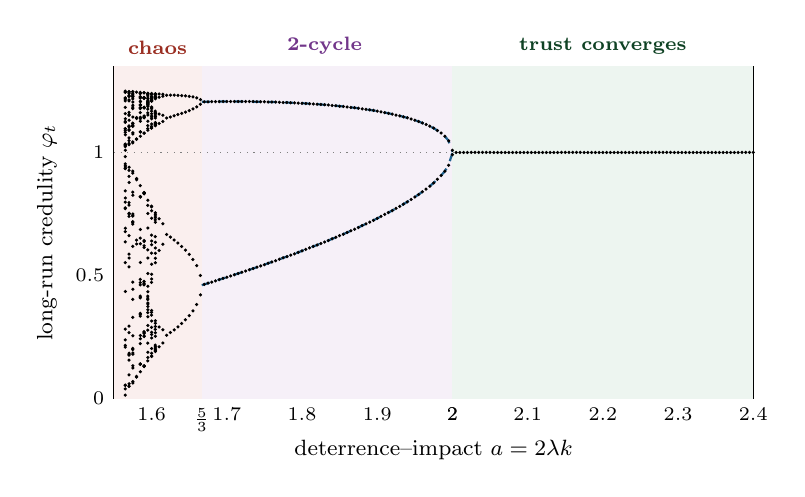
\begin{tikzpicture}
\begin{axis}[width=0.8\textwidth, height=5.8cm, xmin=1.55, xmax=2.4, ymin=0, ymax=1.35,
  xlabel={\footnotesize deterrence--impact $a=2\lambda k$},
  ylabel={\footnotesize long-run credulity $\varphi_t$},
  tick label style={font=\scriptsize}, clip=false]
\fill[echo!8] (axis cs:1.55,0) rectangle (axis cs:1.6667,1.35);
\fill[say!8] (axis cs:1.6667,0) rectangle (axis cs:2,1.35);
\fill[good!8] (axis cs:2,0) rectangle (axis cs:2.4,1.35);
\addplot[only marks, mark=*, mark size=0.35pt, black] coordinates {(1.565,0.014) (1.565,0.039) (1.565,0.053) (1.565,0.054) (1.565,0.209) (1.565,0.216) (1.565,0.238) (1.565,0.282) (1.565,0.435) (1.565,0.552) (1.565,0.637) (1.565,0.678) (1.565,0.692) (1.565,0.772) (1.565,0.775) (1.565,0.798) (1.565,0.815) (1.565,0.844) (1.565,0.934) (1.565,0.935) (1.565,0.941) (1.565,0.946) (1.565,0.954) (1.565,0.983) (1.565,1.009) (1.565,1.024) (1.565,1.028) (1.565,1.03) (1.565,1.033) (1.565,1.034) (1.565,1.072) (1.565,1.082) (1.565,1.089) (1.565,1.096) (1.565,1.097) (1.565,1.122) (1.565,1.126) (1.565,1.137) (1.565,1.158) (1.565,1.183) (1.565,1.21) (1.565,1.217) (1.565,1.221) (1.565,1.222) (1.565,1.244) (1.565,1.246) (1.565,1.249) (1.57,0.049) (1.57,0.05) (1.57,0.06) (1.57,0.096) (1.57,0.156) (1.57,0.176) (1.57,0.178) (1.57,0.184) (1.57,0.268) (1.57,0.294) (1.57,0.535) (1.57,0.571) (1.57,0.587) (1.57,0.662) (1.57,0.74) (1.57,0.75) (1.57,0.751) (1.57,0.753) (1.57,0.786) (1.57,0.796) (1.57,0.878) (1.57,0.903) (1.57,0.927) (1.57,0.94) (1.57,1.032) (1.57,1.037) (1.57,1.048) (1.57,1.059) (1.57,1.09) (1.57,1.093) (1.57,1.104) (1.57,1.105) (1.57,1.108) (1.57,1.131) (1.57,1.151) (1.57,1.154) (1.57,1.163) (1.57,1.21) (1.57,1.214) (1.57,1.228) (1.57,1.229) (1.57,1.232) (1.57,1.24) (1.57,1.245) (1.57,1.246) (1.57,1.247) (1.575,0.063) (1.575,0.069) (1.575,0.124) (1.575,0.133) (1.575,0.18) (1.575,0.185) (1.575,0.199) (1.575,0.204) (1.575,0.255) (1.575,0.33) (1.575,0.403) (1.575,0.444) (1.575,0.473) (1.575,0.618) (1.575,0.709) (1.575,0.715) (1.575,0.719) (1.575,0.741) (1.575,0.744) (1.575,0.75) (1.575,0.826) (1.575,0.839) (1.575,0.916) (1.575,0.924) (1.575,1.039) (1.575,1.043) (1.575,1.075) (1.575,1.08) (1.575,1.106) (1.575,1.108) (1.575,1.109) (1.575,1.116) (1.575,1.117) (1.575,1.119) (1.575,1.144) (1.575,1.178) (1.575,1.184) (1.575,1.192) (1.575,1.205) (1.575,1.218) (1.575,1.226) (1.575,1.227) (1.575,1.229) (1.575,1.23) (1.575,1.237) (1.575,1.238) (1.575,1.246) (1.575,1.247) (1.58,0.087) (1.58,0.09) (1.58,0.628) (1.58,0.644) (1.58,0.889) (1.58,0.894) (1.58,1.053) (1.58,1.055) (1.58,1.138) (1.58,1.142) (1.58,1.245) (1.585,0.109) (1.585,0.139) (1.585,0.14) (1.585,0.141) (1.585,0.223) (1.585,0.243) (1.585,0.256) (1.585,0.335) (1.585,0.342) (1.585,0.346) (1.585,0.409) (1.585,0.412) (1.585,0.416) (1.585,0.462) (1.585,0.471) (1.585,0.484) (1.585,0.553) (1.585,0.629) (1.585,0.652) (1.585,0.687) (1.585,0.819) (1.585,0.82) (1.585,0.821) (1.585,0.865) (1.585,1.066) (1.585,1.083) (1.585,1.084) (1.585,1.127) (1.585,1.137) (1.585,1.143) (1.585,1.162) (1.585,1.178) (1.585,1.181) (1.585,1.183) (1.585,1.192) (1.585,1.193) (1.585,1.194) (1.585,1.206) (1.585,1.208) (1.585,1.221) (1.585,1.224) (1.585,1.227) (1.585,1.239) (1.585,1.24) (1.585,1.244) (1.59,0.13) (1.59,0.131) (1.59,0.132) (1.59,0.133) (1.59,0.252) (1.59,0.254) (1.59,0.264) (1.59,0.268) (1.59,0.272) (1.59,0.462) (1.59,0.465) (1.59,0.467) (1.59,0.474) (1.59,0.476) (1.59,0.614) (1.59,0.621) (1.59,0.638) (1.59,0.642) (1.59,0.832) (1.59,0.833) (1.59,0.834) (1.59,0.836) (1.59,0.837) (1.59,1.078) (1.59,1.079) (1.59,1.141) (1.59,1.142) (1.59,1.147) (1.59,1.148) (1.59,1.181) (1.59,1.182) (1.59,1.183) (1.59,1.184) (1.59,1.22) (1.59,1.221) (1.59,1.222) (1.59,1.223) (1.59,1.224) (1.59,1.242) (1.59,1.243) (1.595,0.153) (1.595,0.167) (1.595,0.188) (1.595,0.225) (1.595,0.278) (1.595,0.297) (1.595,0.332) (1.595,0.349) (1.595,0.361) (1.595,0.374) (1.595,0.384) (1.595,0.388) (1.595,0.402) (1.595,0.408) (1.595,0.416) (1.595,0.434) (1.595,0.456) (1.595,0.508) (1.595,0.571) (1.595,0.604) (1.595,0.693) (1.595,0.752) (1.595,0.785) (1.595,0.806) (1.595,1.09) (1.595,1.097) (1.595,1.109) (1.595,1.127) (1.595,1.152) (1.595,1.161) (1.595,1.176) (1.595,1.187) (1.595,1.192) (1.595,1.195) (1.595,1.197) (1.595,1.198) (1.595,1.201) (1.595,1.202) (1.595,1.204) (1.595,1.206) (1.595,1.208) (1.595,1.212) (1.595,1.218) (1.595,1.221) (1.595,1.23) (1.595,1.236) (1.595,1.239) (1.595,1.241) (1.6,0.171) (1.6,0.173) (1.6,0.184) (1.6,0.203) (1.6,0.246) (1.6,0.26) (1.6,0.269) (1.6,0.289) (1.6,0.315) (1.6,0.339) (1.6,0.35) (1.6,0.358) (1.6,0.472) (1.6,0.486) (1.6,0.505) (1.6,0.546) (1.6,0.591) (1.6,0.625) (1.6,0.64) (1.6,0.664) (1.6,0.733) (1.6,0.763) (1.6,0.779) (1.6,0.782) (1.6,1.099) (1.6,1.1) (1.6,1.106) (1.6,1.116) (1.6,1.137) (1.6,1.144) (1.6,1.148) (1.6,1.157) (1.6,1.168) (1.6,1.178) (1.6,1.182) (1.6,1.185) (1.6,1.208) (1.6,1.21) (1.6,1.212) (1.6,1.216) (1.6,1.221) (1.6,1.224) (1.6,1.226) (1.6,1.228) (1.6,1.235) (1.6,1.238) (1.6,1.24) (1.605,0.191) (1.605,0.195) (1.605,0.2) (1.605,0.205) (1.605,0.21) (1.605,0.217) (1.605,0.253) (1.605,0.267) (1.605,0.281) (1.605,0.293) (1.605,0.306) (1.605,0.316) (1.605,0.552) (1.605,0.57) (1.605,0.59) (1.605,0.612) (1.605,0.635) (1.605,0.658) (1.605,0.716) (1.605,0.726) (1.605,0.735) (1.605,0.742) (1.605,0.749) (1.605,0.755) (1.605,1.109) (1.605,1.111) (1.605,1.114) (1.605,1.116) (1.605,1.119) (1.605,1.122) (1.605,1.14) (1.605,1.146) (1.605,1.152) (1.605,1.158) (1.605,1.163) (1.605,1.168) (1.605,1.218) (1.605,1.22) (1.605,1.222) (1.605,1.224) (1.605,1.226) (1.605,1.229) (1.605,1.235) (1.605,1.236) (1.605,1.237) (1.605,1.238) (1.605,1.239) (1.61,0.21) (1.61,0.291) (1.61,0.602) (1.61,0.731) (1.61,1.118) (1.61,1.156) (1.61,1.224) (1.61,1.238) (1.615,0.226) (1.615,0.279) (1.615,0.627) (1.615,0.71) (1.615,1.126) (1.615,1.151) (1.615,1.228) (1.615,1.237) (1.62,0.257) (1.62,0.667) (1.62,1.14) (1.62,1.233) (1.625,0.268) (1.625,0.656) (1.625,1.144) (1.625,1.233) (1.63,0.279) (1.63,0.644) (1.63,1.149) (1.63,1.233) (1.635,0.291) (1.635,0.632) (1.635,1.154) (1.635,1.232) (1.64,0.305) (1.64,0.618) (1.64,1.159) (1.64,1.231) (1.645,0.32) (1.645,0.603) (1.645,1.164) (1.645,1.23) (1.65,0.337) (1.65,0.586) (1.65,1.17) (1.65,1.228) (1.655,0.356) (1.655,0.565) (1.655,1.177) (1.655,1.226) (1.66,0.382) (1.66,0.54) (1.66,1.185) (1.66,1.222) (1.665,0.421) (1.665,0.5) (1.665,1.196) (1.665,1.215) (1.67,0.464) (1.67,1.206) (1.675,0.469) (1.675,1.206) (1.68,0.473) (1.68,1.207) (1.685,0.478) (1.685,1.207) (1.69,0.483) (1.69,1.207) (1.695,0.488) (1.695,1.207) (1.7,0.493) (1.7,1.207) (1.705,0.498) (1.705,1.207) (1.71,0.503) (1.71,1.207) (1.715,0.508) (1.715,1.207) (1.72,0.513) (1.72,1.207) (1.725,0.518) (1.725,1.207) (1.73,0.523) (1.73,1.207) (1.735,0.528) (1.735,1.207) (1.74,0.534) (1.74,1.206) (1.745,0.539) (1.745,1.206) (1.75,0.544) (1.75,1.206) (1.755,0.55) (1.755,1.205) (1.76,0.555) (1.76,1.205) (1.765,0.56) (1.765,1.205) (1.77,0.566) (1.77,1.204) (1.775,0.572) (1.775,1.203) (1.78,0.577) (1.78,1.203) (1.785,0.583) (1.785,1.202) (1.79,0.588) (1.79,1.202) (1.795,0.594) (1.795,1.201) (1.8,0.6) (1.8,1.2) (1.805,0.606) (1.805,1.199) (1.81,0.612) (1.81,1.198) (1.815,0.618) (1.815,1.197) (1.82,0.624) (1.82,1.196) (1.825,0.63) (1.825,1.195) (1.83,0.636) (1.83,1.194) (1.835,0.642) (1.835,1.193) (1.84,0.649) (1.84,1.191) (1.845,0.655) (1.845,1.19) (1.85,0.662) (1.85,1.188) (1.855,0.668) (1.855,1.187) (1.86,0.675) (1.86,1.185) (1.865,0.682) (1.865,1.183) (1.87,0.688) (1.87,1.182) (1.875,0.695) (1.875,1.18) (1.88,0.703) (1.88,1.177) (1.885,0.71) (1.885,1.175) (1.89,0.717) (1.89,1.173) (1.895,0.724) (1.895,1.171) (1.9,0.732) (1.9,1.168) (1.905,0.74) (1.905,1.165) (1.91,0.748) (1.91,1.162) (1.915,0.756) (1.915,1.159) (1.92,0.764) (1.92,1.156) (1.925,0.773) (1.925,1.152) (1.93,0.781) (1.93,1.149) (1.935,0.79) (1.935,1.145) (1.94,0.799) (1.94,1.141) (1.945,0.809) (1.945,1.136) (1.95,0.819) (1.95,1.131) (1.955,0.829) (1.955,1.126) (1.96,0.84) (1.96,1.12) (1.965,0.851) (1.965,1.114) (1.97,0.863) (1.97,1.107) (1.975,0.876) (1.975,1.099) (1.98,0.891) (1.98,1.089) (1.985,0.906) (1.985,1.079) (1.99,0.924) (1.99,1.066) (1.995,0.948) (1.995,1.047) (2.0,0.991) (2.0,1.009) (2.005,1.0) (2.01,1.0) (2.015,1.0) (2.02,1.0) (2.025,1.0) (2.03,1.0) (2.035,1.0) (2.04,1.0) (2.045,1.0) (2.05,1.0) (2.055,1.0) (2.06,1.0) (2.065,1.0) (2.07,1.0) (2.075,1.0) (2.08,1.0) (2.085,1.0) (2.09,1.0) (2.095,1.0) (2.1,1.0) (2.105,1.0) (2.11,1.0) (2.115,1.0) (2.12,1.0) (2.125,1.0) (2.13,1.0) (2.135,1.0) (2.14,1.0) (2.145,1.0) (2.15,1.0) (2.155,1.0) (2.16,1.0) (2.165,1.0) (2.17,1.0) (2.175,1.0) (2.18,1.0) (2.185,1.0) (2.19,1.0) (2.195,1.0) (2.2,1.0) (2.205,1.0) (2.21,1.0) (2.215,1.0) (2.22,1.0) (2.225,1.0) (2.23,1.0) (2.235,1.0) (2.24,1.0) (2.245,1.0) (2.25,1.0) (2.255,1.0) (2.26,1.0) (2.265,1.0) (2.27,1.0) (2.275,1.0) (2.28,1.0) (2.285,1.0) (2.29,1.0) (2.295,1.0) (2.3,1.0) (2.305,1.0) (2.31,1.0) (2.315,1.0) (2.32,1.0) (2.325,1.0) (2.33,1.0) (2.335,1.0) (2.34,1.0) (2.345,1.0) (2.35,1.0) (2.355,1.0) (2.36,1.0) (2.365,1.0) (2.37,1.0) (2.375,1.0) (2.38,1.0) (2.385,1.0) (2.39,1.0) (2.395,1.0) (2.4,1.0)};
\addplot[do, thick, dashed, domain=1.6667:2, samples=60] {(x+sqrt(x*(2-x)))/2};
\addplot[do, thick, dashed, domain=1.6667:2, samples=60] {(x-sqrt(x*(2-x)))/2};
\addplot[gray, thin, dotted] coordinates {(1.55,1) (2.4,1)};
\node[font=\scriptsize\bfseries, text=good!50!black, anchor=south] at (axis cs:2.2,1.36) {trust converges};
\node[font=\scriptsize\bfseries, text=say!80!black, anchor=south] at (axis cs:1.83,1.36) {2-cycle};
\node[font=\scriptsize\bfseries, text=echo!80!black, anchor=south] at (axis cs:1.608,1.36) {chaos};
\node[font=\scriptsize, anchor=north] at (axis cs:1.6667,0) {$\tfrac53$};
\node[font=\scriptsize, anchor=north] at (axis cs:2,0) {$2$};
\end{axis}
\end{tikzpicture}
\caption{Bifurcation diagram of adaptive trust (\cref{thm:cycles}); dots show the long-run attractor, and dashed curves the closed-form $2$-cycle $\varphi_\pm$. Above $a=2$ trust converges to truth. Between $\tfrac53$ and $2$ the market alternates between under- and over-trust. Below $\tfrac53$ further period-doublings lead to chaotic trust (numerical Lyapunov exponent $\approx0.10$ at $a=1.6$), and for $a\lesssim1.56$ the orbit leaves the admissible set: credibility collapses.}
\label{fig:bifurcation}
\end{figure}

\begin{remark}[Relation to reputation models]
\citet{benabou1992} obtain credibility dynamics from Bayesian updating about a random honest type. Here the dynamics arise from a deterministic cobweb in credulity, and the thresholds $\lambda k=1$ and $\lambda k=\tfrac56$ are explicit. The mechanism is the same as the period-doubling route to chaos in simple nonlinear maps \citep{may1976}. The prediction is new and testable: the rolling Say--Do covariance should be negatively autocorrelated in markets where the product of price impact and misreporting cost is moderate.
\end{remark}

% =====================================================================
\section{Echo: Exact Decomposition of Media Sentiment}\label{sec:echo}

Let articles about an asset arrive at times $0<\tau_1<\dots<\tau_N\le T$ with sentiment marks $s_1,\dots,s_N$.

\begin{definition}[Linear Hawkes process]
A simple point process on $[0,T]$ with conditional intensity
\[
  \lambda(t)=\mu+\sum_{\tau_l<t}g(t-\tau_l),\qquad \mu>0,\ g\ge0,\ n\coloneqq\int_0^\infty g(s)\,ds<1 .
\]
For the exponential kernel $g(s)=\alpha e^{-\beta_g s}$, the branching ratio is $n=\alpha/\beta_g$.
\end{definition}

By the cluster representation \citep{hawkesoakes1974}, the process is the superposition of an immigrant Poisson stream of rate $\mu$ (\emph{news}) and, for each point $\tau_l$, an offspring Poisson stream of rate $g(\cdot-\tau_l)$ on $(\tau_l,T]$ (\emph{echo}). Let $\pi(j)\in\{0,1,\dots,j-1\}$ denote the parent of article $j$, with $\pi(j)=0$ meaning immigrant.

\begin{figure}[ht]
\centering
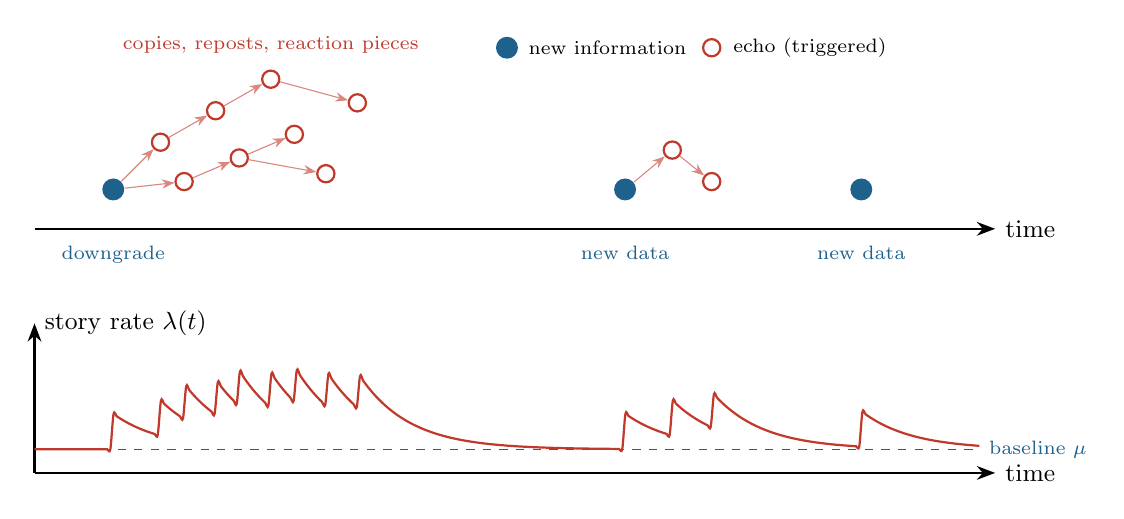
\begin{tikzpicture}[
  newn/.style={circle, fill=do, inner sep=2.8pt},
  echn/.style={circle, draw=echo, thick, fill=white, inner sep=2.2pt},
  trig/.style={-{Stealth[length=1.6mm]}, echo!60, thin}]
% time axis for cascade
\draw[-{Stealth}, thick] (0,0) -- (12.2,0) node[right, font=\small] {time};
% first cascade
\node[newn] (a) at (1,0.5) {};
\node[echn] (a1) at (1.6,1.1) {};
\node[echn] (a2) at (1.9,0.6) {};
\node[echn] (a3) at (2.3,1.5) {};
\node[echn] (a4) at (2.6,0.9) {};
\node[echn] (a5) at (3.0,1.9) {};
\node[echn] (a6) at (3.3,1.2) {};
\node[echn] (a7) at (3.7,0.7) {};
\node[echn] (a8) at (4.1,1.6) {};
\draw[trig] (a) -- (a1); \draw[trig] (a) -- (a2); \draw[trig] (a1) -- (a3);
\draw[trig] (a2) -- (a4); \draw[trig] (a3) -- (a5); \draw[trig] (a4) -- (a6);
\draw[trig] (a4) -- (a7); \draw[trig] (a5) -- (a8);
% second cascade
\node[newn] (b) at (7.5,0.5) {};
\node[echn] (b1) at (8.1,1.0) {};
\node[echn] (b2) at (8.6,0.6) {};
\draw[trig] (b) -- (b1); \draw[trig] (b1) -- (b2);
% lone new story
\node[newn] (c) at (10.5,0.5) {};
% labels
\node[font=\scriptsize, text=do, anchor=north] at (1,-0.1) {downgrade};
\node[font=\scriptsize, text=echo, anchor=south] at (3.0,2.1) {copies, reposts, reaction pieces};
\node[font=\scriptsize, text=do, anchor=north] at (7.5,-0.1) {new data};
\node[font=\scriptsize, text=do, anchor=north] at (10.5,-0.1) {new data};
% intensity curve
\begin{scope}[yshift=-3.1cm]
\draw[-{Stealth}, thick] (0,0) -- (12.2,0) node[right, font=\small] {time};
\draw[-{Stealth}, thick] (0,0) -- (0,1.9) node[right, font=\small] {story rate $\lambda(t)$};
\draw[dashed, do] (0,0.3) -- (12,0.3) node[right, font=\scriptsize, text=do] {baseline $\mu$};
\draw[echo, thick, smooth, samples=300, domain=0:12] plot (\x, {0.3
  + 0.45*(\x>1.0)*exp(-1.6*max(\x-1.0,0)) + 0.45*(\x>1.6)*exp(-1.6*max(\x-1.6,0))
  + 0.45*(\x>1.9)*exp(-1.6*max(\x-1.9,0)) + 0.45*(\x>2.3)*exp(-1.6*max(\x-2.3,0))
  + 0.45*(\x>2.6)*exp(-1.6*max(\x-2.6,0)) + 0.45*(\x>3.0)*exp(-1.6*max(\x-3.0,0))
  + 0.45*(\x>3.3)*exp(-1.6*max(\x-3.3,0)) + 0.45*(\x>3.7)*exp(-1.6*max(\x-3.7,0))
  + 0.45*(\x>4.1)*exp(-1.6*max(\x-4.1,0)) + 0.45*(\x>7.5)*exp(-1.6*max(\x-7.5,0))
  + 0.45*(\x>8.1)*exp(-1.6*max(\x-8.1,0)) + 0.45*(\x>8.6)*exp(-1.6*max(\x-8.6,0))
  + 0.45*(\x>10.5)*exp(-1.6*max(\x-10.5,0))});
\end{scope}
% legend
\node[newn] at (6.0,2.3) {}; \node[font=\scriptsize, anchor=west] at (6.15,2.3) {new information};
\node[echn] at (8.6,2.3) {}; \node[font=\scriptsize, anchor=west] at (8.75,2.3) {echo (triggered)};
\end{tikzpicture}
\caption{Echo versus news. Top: each new article (blue) triggers a cascade of echoes (red). Bottom: the intensity jumps with every arrival and decays to the baseline $\mu$. \Cref{prop:parentage} assigns each article its exact posterior probability of being news.}
\label{fig:cascade}
\end{figure}

\begin{proposition}[Posterior parentage factorises; cf.\ \citealp{zhuang2002}]\label{prop:parentage}
Conditionally on the full sample $\mathcal{T}=\{\tau_1,\dots,\tau_N\}$ on $[0,T]$, the parent labels $\pi(1),\dots,\pi(N)$ are independent, with
\[
  \Prob\big(\pi(j)=0\mid\mathcal{T}\big)=\frac{\mu}{\lambda(\tau_j)}\eqqcolon p_j,\qquad
  \Prob\big(\pi(j)=l\mid\mathcal{T}\big)=\frac{g(\tau_j-\tau_l)}{\lambda(\tau_j)},\quad l<j .
\]
\end{proposition}
\begin{proof}
Write $\rho_0(t)=\mu$ and $\rho_l(t)=g(t-\tau_l)\ind\{t>\tau_l\}$. In the cluster representation, a labelled configuration is a realisation of the independent Poisson streams, so its density with respect to the reference measure of labelled configurations is the product of the Poisson likelihoods of the streams,
\[
  \prod_{k}\Big[\exp\Big(-\int_0^T\rho_k\Big)\prod_{j:\pi(j)=k}\rho_k(\tau_j)\Big]
  =\exp\Big(-\int_0^T\lambda(t)\,dt\Big)\prod_{j=1}^N\rho_{\pi(j)}(\tau_j),
\]
because $\sum_k\rho_k(t)=\lambda(t)$. Summing over labellings, the product factorises over $j$, and $\sum_k\rho_k(\tau_j)=\lambda(\tau_j)$ recovers the standard Hawkes likelihood $e^{-\int\lambda}\prod_j\lambda(\tau_j)$. Dividing, the posterior of the labelling is $\prod_j\rho_{\pi(j)}(\tau_j)/\lambda(\tau_j)$, a product of independent categorical laws.
\end{proof}

\begin{remark}
The posterior uses only the past of $\tau_j$, although it conditions on the whole sample: future arrivals are informative about \emph{their} parents, not about $\pi(j)$. The echo split is therefore causal and free of look-ahead \citep[cf.][]{zhuang2002}.
\end{remark}

\begin{proposition}[Branching ratio is the long-run echo share]\label{prop:branching}
For the stationary process ($n<1$), the mean intensity is $\Lambda=\mu/(1-n)$, and the long-run fraction of articles that are echoes equals $n$.
\end{proposition}
\begin{proof}
Each immigrant founds a Galton--Watson cluster whose generations have expected sizes $1,n,n^2,\dots$, so its expected total size is $(1-n)^{-1}$. Immigrants arrive at rate $\mu$, so articles arrive at rate $\Lambda=\mu/(1-n)$ (equivalently, stationarity gives $\Lambda=\mu+\Lambda\int g$). The immigrant fraction is $\mu/\Lambda=1-n$.
\end{proof}

\begin{proposition}[MMSE news--echo split]\label{prop:mmse}
Assume that, given $\mathcal{T}$, the marks are independent of the labels. Then the minimum-mean-square-error estimates of the news and echo sentiment totals are
\[
  s^{\text{new}}\coloneqq\E\Big[\sum_j\ind\{\pi(j)=0\}s_j\,\Big|\,\mathcal{T},\bm s\Big]=\sum_j p_j s_j,\qquad
  s^{\text{echo}}=\sum_j(1-p_j)s_j .
\]
\end{proposition}
\begin{proof}
Conditional expectation minimises mean-square error. By linearity and the assumption, $\E[\ind\{\pi(j)=0\}s_j\mid\mathcal{T},\bm s]=s_j\Prob(\pi(j)=0\mid\mathcal{T})=p_js_j$, using \cref{prop:parentage}.
\end{proof}

\begin{intuition}
Combining \cref{cor:echo} with \cref{prop:mmse}: $s^{\text{echo}}$ estimates exactly the garbled component that the crowd should not have priced, so it enters forecasts with a negative sign, while $s^{\text{new}}$ enters with the sign set by \cref{cor:news}.
\end{intuition}


\subsection{Semantic declustering: timing and meaning together}\label{sec:semantic}

\Cref{prop:mmse} needs marks that are uninformative about parentage, and real echoes are not: a reprint \emph{looks like} its parent. We therefore let the parent's embedding shape the child's.

\begin{assumption}[Semantically marked cascade]\label{ass:marked}
In the cluster representation, immigrant articles carry embeddings $\z\sim f_0$ independently, and an offspring of article $l$ carries $\z\sim f(\cdot\mid\z_l)$, for example the von Mises--Fisher density $f(\z\mid\z_l)=C_D(\varkappa)\,e^{\varkappa\langle\z,\z_l\rangle}$ on $S^{D-1}$. Marks are conditionally independent given the parent labels.
\end{assumption}

\begin{theorem}[Semantic declustering]\label{thm:semantic}
Under \cref{ass:marked}, conditionally on all times and embeddings $(\mathcal{T},\z_{1:N})$ observed on $[0,T]$, the parent labels are independent, with
\[
  \Prob(\pi(j)=0\mid\cdot)=\frac{\mu f_0(\z_j)}{\Lambda_j},\qquad
  \Prob(\pi(j)=l\mid\cdot)=\frac{g(\tau_j-\tau_l)\,f(\z_j\mid\z_l)}{\Lambda_j},
\]
where $\Lambda_j=\mu f_0(\z_j)+\sum_{l<j}g(\tau_j-\tau_l)f(\z_j\mid\z_l)$.
Consequently, (i) the MMSE news--echo split of \cref{prop:mmse} holds \emph{without} the independence assumption, with $p_j$ replaced by $p_j^{\text{sem}}=\mu f_0(\z_j)/\Lambda_j$; and (ii) the expected posterior entropy of each parent label is no larger than under timing alone: $\E\,H(\pi(j)\mid\mathcal{T},\z)\le\E\,H(\pi(j)\mid\mathcal{T})$.
\end{theorem}
\begin{proof}
As in \cref{prop:parentage}, the density of a labelled configuration is the product of the stream likelihoods times the mark densities, $e^{-\int_0^T\lambda}\prod_j\rho_{\pi(j)}(\tau_j)\,f_{\pi(j)}(\z_j)$, where $f_0$ is the immigrant mark density and $f_l=f(\cdot\mid\z_l)$. This factorises over $j$; summing over labellings gives $e^{-\int\lambda}\prod_j\Lambda_j$, and the posterior is the product of the stated categorical laws. For (i), marks are now conditioned on, so no independence assumption is needed: $\E[\ind\{\pi(j)=0\}s_j\mid\mathcal{T},\z]=s_j\,p^{\text{sem}}_j$ whenever $s_j$ is a function of $\z_j$, as it is for $s_j=\langle\w_s^\perp,\z_j\rangle$. For (ii), integrating the marks out sequentially shows that the timing-only posterior is that of \cref{prop:parentage}, and conditioning does not increase expected entropy.
\end{proof}

\begin{figure}[ht]
\centering
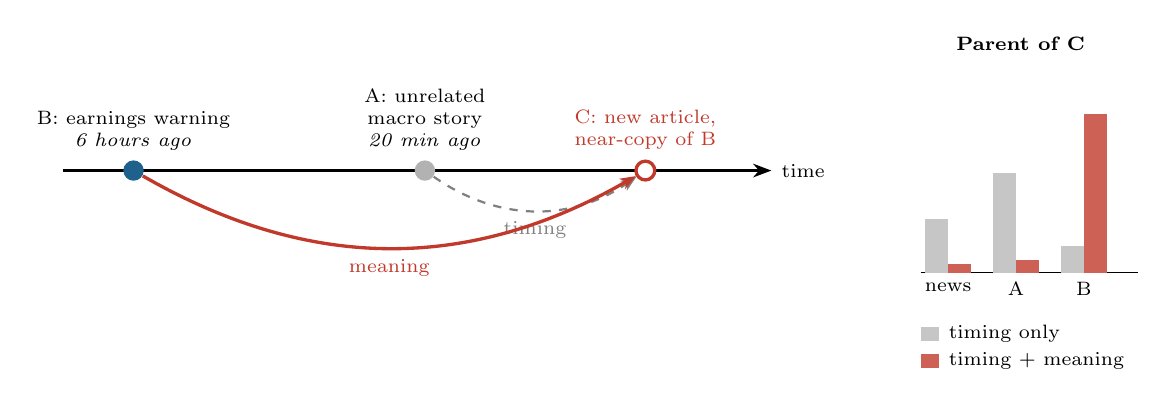
\begin{tikzpicture}[font=\small]
\draw[-{Stealth}, thick] (0,0) -- (9.0,0) node[right, font=\scriptsize] {time};
\node[circle, fill=do, inner sep=2.6pt, label={[font=\scriptsize, align=center]above:{B: earnings warning\\ \textit{6 hours ago}}}] (B) at (0.9,0) {};
\node[circle, fill=gray!60, inner sep=2.6pt, label={[font=\scriptsize, align=center]above:{A: unrelated\\ macro story\\ \textit{20 min ago}}}] (A) at (4.6,0) {};
\node[circle, draw=echo, very thick, fill=white, inner sep=2.4pt, label={[font=\scriptsize, align=center, text=echo]above:{C: new article,\\ near-copy of B}}] (C) at (7.4,0) {};
\draw[-{Stealth[length=2mm]}, thick, gray, dashed] (A) to[out=-35,in=-145] node[below, font=\scriptsize, text=gray] {timing} (C);
\draw[-{Stealth[length=2mm]}, very thick, echo] (B) to[out=-30,in=-150] node[below, font=\scriptsize, text=echo] {meaning} (C);
% bars
\begin{scope}[xshift=10.9cm, yshift=-1.3cm, scale=1.15]
\node[font=\scriptsize\bfseries, anchor=south] at (1.1,2.35) {Parent of C};
\foreach \lab/\x in {news/0, A/0.75, B/1.5} {\node[font=\scriptsize, anchor=north] at (\x+0.3,0) {\lab};}
\draw (0,0) -- (2.4,0);
\fill[gray!45] (0.05,0) rectangle (0.3,0.60);  \fill[echo!80] (0.3,0) rectangle (0.55,0.10);
\fill[gray!45] (0.80,0) rectangle (1.05,1.10); \fill[echo!80] (1.05,0) rectangle (1.30,0.14);
\fill[gray!45] (1.55,0) rectangle (1.80,0.30); \fill[echo!80] (1.80,0) rectangle (2.05,1.76);
\fill[gray!45] (0,-0.75) rectangle (0.2,-0.6); \node[font=\scriptsize, anchor=west] at (0.2,-0.675) {timing only};
\fill[echo!80] (0,-1.05) rectangle (0.2,-0.9); \node[font=\scriptsize, anchor=west] at (0.2,-0.975) {timing + meaning};
\end{scope}
\end{tikzpicture}
\caption{Semantic declustering (\cref{thm:semantic}), illustrative numbers. Timing alone attributes article C to the most recent story A. Adding embedding similarity attributes it to B, of which it is a near-copy. C is thus correctly classified as echo of B, and its sentiment enters $s^{\text{echo}}$.}
\label{fig:semantic}
\end{figure}

% =====================================================================
\section{Market-Aligned Embeddings}\label{sec:embeddings}

An embedding model maps each document to a point on the unit sphere $\z\in S^{D-1}$. On this \emph{map of meaning}, directions carry concepts and distances carry surprise (\cref{fig:map}).

\begin{figure}[ht]
\centering
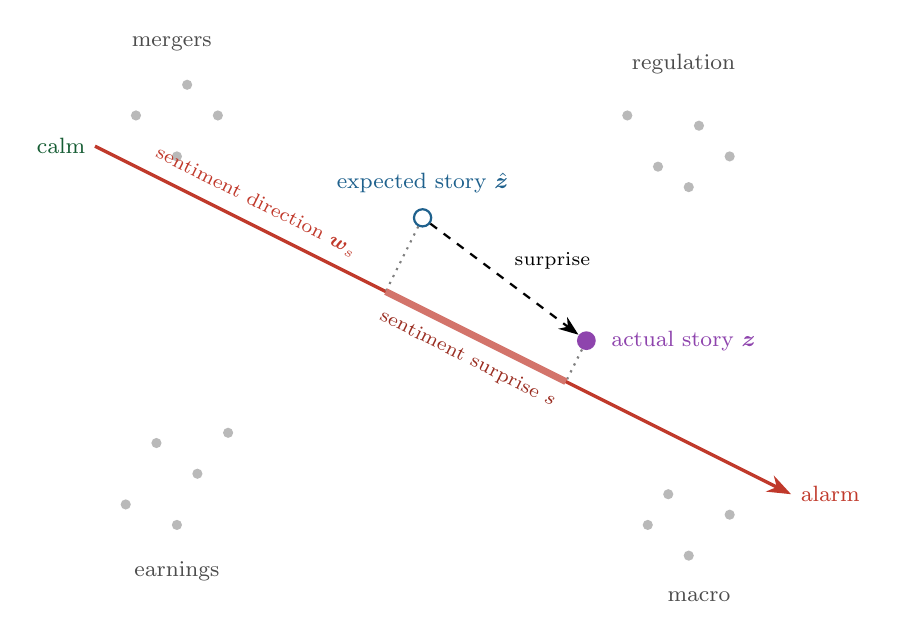
\begin{tikzpicture}[scale=1.3, dot/.style={circle, fill=gray!55, inner sep=1.3pt}]
\foreach \p in {(-2.6,-1.3),(-2.2,-1.6),(-2.9,-1.9),(-2.4,-2.1),(-1.9,-1.2)} \node[dot] at \p {};
\node[font=\footnotesize, text=gray!60!black] at (-2.4,-2.55) {earnings};
\foreach \p in {(-2.4,1.5),(-2.0,1.9),(-2.8,1.9),(-2.3,2.2)} \node[dot] at \p {};
\node[font=\footnotesize, text=gray!60!black] at (-2.45,2.6) {mergers};
\foreach \p in {(2.3,1.4),(2.7,1.8),(2.0,1.9),(2.6,1.2),(3.0,1.5)} \node[dot] at \p {};
\node[font=\footnotesize, text=gray!60!black] at (2.55,2.4) {regulation};
\foreach \p in {(2.2,-2.1),(2.6,-2.4),(3.0,-2.0),(2.4,-1.8)} \node[dot] at \p {};
\node[font=\footnotesize, text=gray!60!black] at (2.7,-2.8) {macro};
\draw[-{Stealth[length=3mm]}, echo, very thick] (-3.2,1.6) -- (3.6,-1.8);
\node[font=\footnotesize, text=echo, anchor=west] at (3.6,-1.8) {alarm};
\node[font=\footnotesize, text=good!70!black, anchor=east] at (-3.2,1.6) {calm};
\node[font=\scriptsize, text=echo, rotate=-26.6, anchor=south] at (-1.7,0.9) {sentiment direction $\w_s$};
\node[circle, draw=do, thick, fill=white, inner sep=2.2pt] (ez) at (0,0.9) {};
\node[circle, fill=say, inner sep=2.4pt] (az) at (1.6,-0.3) {};
\node[font=\footnotesize, text=do, anchor=south] at (0,1.05) {expected story $\hat{\z}$};
\node[font=\footnotesize, text=say, anchor=west] at (1.75,-0.3) {actual story $\z$};
\draw[-{Stealth[length=2.5mm]}, dashed, thick] (ez) -- (az) node[midway, above right, font=\scriptsize] {surprise};
\draw[dotted, thick, gray] (ez) -- (-0.36,0.18);
\draw[dotted, thick, gray] (az) -- (1.40,-0.70);
\draw[line width=2.5pt, echo!70] (-0.36,0.18) -- (1.40,-0.70);
\node[font=\scriptsize, text=echo!80!black, rotate=-26.6, anchor=north] at (0.52,-0.32) {sentiment surprise $s$};
\end{tikzpicture}
\caption{The map of meaning (a two-dimensional cartoon of a high-dimensional sphere). Sentiment is a direction; surprise is the gap between the expected and the actual story; sentiment surprise is its projection on the alarm direction.}
\label{fig:map}
\end{figure}

\subsection{Return-aligned contrastive learning}

For documents $j=1,\dots,N$ ($N\ge2$) with embeddings $\z_j$ and post-event \emph{response vectors} $\bm\rho_j\in\R^M$ (abnormal returns at several horizons, abnormal volume, change in implied volatility), set $S_{jk}=\langle\z_j,\z_k\rangle$, $D_{jk}=\|\bm\rho_j-\bm\rho_k\|^2$, and for $k\neq j$
\[
  q_{jk}=\frac{e^{-D_{jk}/2b^2}}{\sum_{l\neq j}e^{-D_{jl}/2b^2}},\qquad
  p_{jk}(Z)=\frac{e^{S_{jk}/\tau}}{\sum_{l\neq j}e^{S_{jl}/\tau}},\qquad
  \mathcal{L}(Z)=-\sum_j\sum_{k\neq j}q_{jk}\log p_{jk}(Z).
\]

\begin{theorem}[Minimisers are affine isometries of outcome space]\label{thm:racl}
$\mathcal{L}(Z)\ge\sum_jH(q_{j\cdot})$, with equality if and only if there is a constant $c\in\R$ such that $S_{jk}=c-\frac{\tau}{2b^2}D_{jk}$ for all $j\neq k$. At equality,
\[
  \|\z_j-\z_k\|^2=2(1-c)+\frac{\tau}{b^2}\,\|\bm\rho_j-\bm\rho_k\|^2\qquad\text{for all } j\neq k .
\]
\end{theorem}
\begin{proof}
For each anchor, $-\sum_kq_{jk}\log p_{jk}=H(q_{j\cdot})+\KL(q_{j\cdot}\|p_{j\cdot})\ge H(q_{j\cdot})$ by Gibbs' inequality, with equality iff $p_{j\cdot}=q_{j\cdot}$. Two softmax vectors coincide iff their logits differ by a constant, so equality holds iff $S_{jk}/\tau+D_{jk}/2b^2=c_j/\tau$ for all $k\neq j$. By symmetry of $S$ and $D$, for every pair $j\neq k$, $c_j=S_{jk}+\tfrac{\tau}{2b^2}D_{jk}=S_{kj}+\tfrac{\tau}{2b^2}D_{kj}=c_k$, so all $c_j$ equal a common $c$. The converse is immediate. On the sphere, $\|\z_j-\z_k\|^2=2-2S_{jk}$.
\end{proof}

\begin{corollary}[Neighbour preservation]\label{cor:order}
At a global minimiser, for every anchor $j$ and $k,l\neq j$: $\|\z_j-\z_k\|<\|\z_j-\z_l\|\iff\|\bm\rho_j-\bm\rho_k\|<\|\bm\rho_j-\bm\rho_l\|$. Nearest neighbours in embedding space are exactly nearest neighbours in market-outcome space.
\end{corollary}

\begin{theorem}[Robust neighbour preservation]\label{thm:robustnn}
Let $Z$ be \emph{any} embedding, and let $\epsilon_j\coloneqq\KL\big(q_{j\cdot}\,\|\,p_{j\cdot}(Z)\big)$ be the excess loss at anchor~$j$. For $k,l\neq j$, each of the following conditions implies $\|\z_j-\z_k\|<\|\z_j-\z_l\|$:
\begin{enumerate}[label=(\roman*)]
  \item \emph{(Pinsker)} $q_{jk}-q_{jl}>\sqrt{2\epsilon_j}$;
  \item \emph{(exact)} $q_{jk}>q_{jl}$ and
  \[
    \Delta_{jkl}\coloneqq q_{jk}\log\frac{2q_{jk}}{q_{jk}+q_{jl}}+q_{jl}\log\frac{2q_{jl}}{q_{jk}+q_{jl}}\;>\;\epsilon_j .
  \]
\end{enumerate}
Condition (i) implies (ii). Condition (ii) is the weakest condition that is valid for every distribution within KL distance $\epsilon_j$ of $q_{j\cdot}$: if $\epsilon_j\ge\Delta_{jkl}$, some such distribution gives $k$ and $l$ equal probability. (Softmax outputs with temperature $\tau$ satisfy $p_{\max}/p_{\min}\le e^{2/\tau}$, and a certificate that used this constraint could be sharper still.)
\end{theorem}
\begin{proof}
Throughout, $p_{j\cdot}$ is a softmax of $S_{j\cdot}/\tau$, so $p_{jk}>p_{jl}$ is equivalent to $S_{jk}>S_{jl}$, and on the sphere $\|\z_j-\z_k\|^2=2-2S_{jk}$. It therefore suffices to show $p_{jk}>p_{jl}$.

(i) By Pinsker's inequality, $\sum_{k}|p_{jk}-q_{jk}|\le\sqrt{2\epsilon_j}$. Hence $p_{jk}-p_{jl}\ge(q_{jk}-q_{jl})-|p_{jk}-q_{jk}|-|p_{jl}-q_{jl}|>0$.

(ii) Merge all outcomes other than $k$ and $l$ into one cell. By the data-processing inequality, the three-cell divergence satisfies $\KL_3(q\|p)\le\epsilon_j$. Consider the set $\{p: p_k\le p_l\}$. The divergence is convex in $p$, and its unconstrained minimiser $p=q$ lies outside this set because $q_{jk}>q_{jl}$. The constrained minimum is therefore attained on the boundary $p_k=p_l=t$, with $p_{\text{rest}}=1-2t$. Setting the derivative in $t$ to zero gives $t=(q_{jk}+q_{jl})/2$ and $p_{\text{rest}}=q_{\text{rest}}$, where the divergence equals $\Delta_{jkl}$. So every $p$ with $p_{jk}\le p_{jl}$ has $\KL_3(q\|p)\ge\Delta_{jkl}>\epsilon_j$, which is impossible. The boundary point with $p_{\text{rest}}$ split in proportion to $q$ shows that the bound is attained, which gives tightness.

For (i)$\Rightarrow$(ii), write $\pi=q_{jk}/(q_{jk}+q_{jl})$. Then $\Delta_{jkl}=(q_{jk}+q_{jl})\,\KL\big(\text{Bern}(\pi)\,\|\,\text{Bern}(\tfrac12)\big)\ge 2(q_{jk}+q_{jl})(\pi-\tfrac12)^2=\frac{(q_{jk}-q_{jl})^2}{2(q_{jk}+q_{jl})}\ge\frac{(q_{jk}-q_{jl})^2}{2}$, by Pinsker for two points and $q_{jk}+q_{jl}\le1$.
\end{proof}

\begin{remark}
\Cref{thm:racl} is the case $\epsilon_j=0$. \Cref{thm:robustnn} makes it quantitative: the training loss that remains after optimisation certifies which analog rankings, and hence which terms of the d\'ej\`a vu estimator of \cref{prop:analog}, can be trusted. Only near-ties in outcome space can be misordered. The exact form matters in practice. With $N$ neighbours, target probabilities are of order $1/N$, and the chain of inequalities above shows that (ii) tolerates an excess loss at least $1/(q_{jk}+q_{jl})$ times larger than (i), which is about $N/2$ times larger. \Cref{sec:experiments} shows that even this is demanding.
\end{remark}


\begin{remark}[Realisability and regularisation]
Equality requires the matrix with unit diagonal and off-diagonal entries $c-\frac{\tau}{2b^2}D_{jk}$ to be positive semidefinite of rank at most $D$. Otherwise the minimiser is the closest realisable geometry in the KL sense. In practice we add a semantic anchor $\sum_j\KL(p^{(0)}_{j\cdot}\|p_{j\cdot})$ to the frozen encoder, which interpolates between topic geometry and outcome geometry.
\end{remark}

\begin{figure}[ht]
\centering
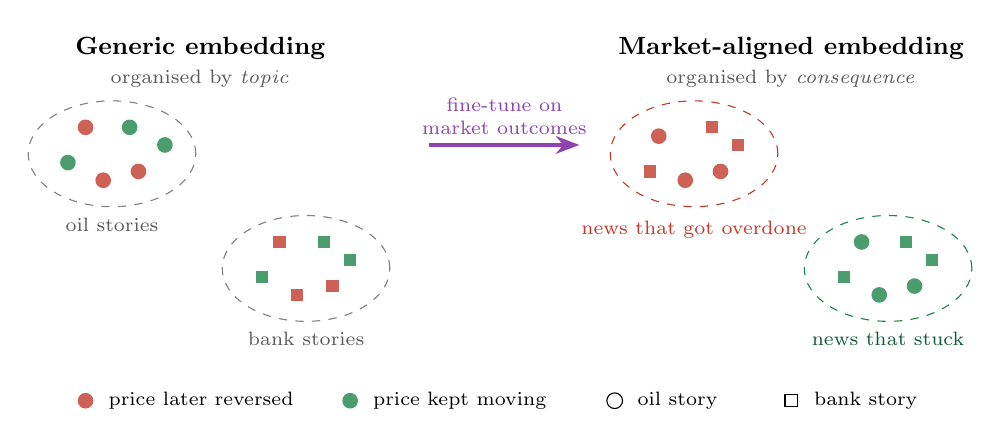
\begin{tikzpicture}[scale=1.12,
  cr/.style={circle, fill=echo!80, inner sep=2pt},
  cg/.style={circle, fill=good!80, inner sep=2pt},
  sr/.style={rectangle, fill=echo!80, inner sep=2.2pt},
  sg/.style={rectangle, fill=good!80, inner sep=2.2pt}]
% left panel
\node[font=\small\bfseries] at (2.3,3.4) {Generic embedding};
\node[font=\scriptsize, text=gray!70!black] at (2.3,3.05) {organised by \emph{topic}};
\draw[dashed, gray] (1.3,2.2) ellipse (0.95 and 0.6);
\draw[dashed, gray] (3.5,0.9) ellipse (0.95 and 0.6);
\node[font=\scriptsize, text=gray!70!black] at (1.3,1.4) {oil stories};
\node[font=\scriptsize, text=gray!70!black] at (3.5,0.1) {bank stories};
\foreach \p in {(1.0,2.5),(1.6,2.0),(1.2,1.9)} \node[cr] at \p {};
\foreach \p in {(1.5,2.5),(0.8,2.1),(1.9,2.3)} \node[cg] at \p {};
\foreach \p in {(3.2,1.2),(3.8,0.7),(3.4,0.6)} \node[sr] at \p {};
\foreach \p in {(3.7,1.2),(3.0,0.8),(4.0,1.0)} \node[sg] at \p {};
% arrow
\draw[-{Stealth[length=3mm]}, very thick, say] (4.9,2.3) -- (6.6,2.3) node[midway, above, font=\scriptsize, align=center] {fine-tune on\\ market outcomes};
% right panel
\node[font=\small\bfseries] at (9.0,3.4) {Market-aligned embedding};
\node[font=\scriptsize, text=gray!70!black] at (9.0,3.05) {organised by \emph{consequence}};
\draw[dashed, echo] (7.9,2.2) ellipse (0.95 and 0.6);
\draw[dashed, good] (10.1,0.9) ellipse (0.95 and 0.6);
\node[font=\scriptsize, text=echo, anchor=north] at (7.9,1.55) {news that got overdone};
\node[font=\scriptsize, text=good!70!black] at (10.1,0.1) {news that stuck};
\foreach \p in {(7.5,2.4),(8.2,2.0),(7.8,1.9)} \node[cr] at \p {};
\foreach \p in {(8.1,2.5),(7.4,2.0),(8.4,2.3)} \node[sr] at \p {};
\foreach \p in {(9.8,1.2),(10.4,0.7),(10.0,0.6)} \node[cg] at \p {};
\foreach \p in {(10.3,1.2),(9.6,0.8),(10.6,1.0)} \node[sg] at \p {};
% legend
\node[cr] at (1.0,-0.6) {}; \node[font=\scriptsize, anchor=west] at (1.15,-0.6) {price later reversed};
\node[cg] at (4.0,-0.6) {}; \node[font=\scriptsize, anchor=west] at (4.15,-0.6) {price kept moving};
\node[circle, draw, inner sep=2pt] at (7.0,-0.6) {}; \node[font=\scriptsize, anchor=west] at (7.15,-0.6) {oil story};
\node[rectangle, draw, inner sep=2.2pt] at (9.0,-0.6) {}; \node[font=\scriptsize, anchor=west] at (9.15,-0.6) {bank story};
\end{tikzpicture}
\caption{\Cref{thm:racl} in pictures. Before fine-tuning, stories cluster by subject. At the optimum, distances mirror market aftermaths, so ``news that got overdone'' becomes a region of the map.}
\label{fig:finetune}
\end{figure}

\subsection{Topic-orthogonal sentiment and calibrated surprise}

\begin{lemma}[Topic invariance]\label{lem:topic}
Let $U\in\R^{D\times r}$ have orthonormal columns spanning topic directions and $\w_s^\perp\coloneqq(I-UU^\top)\w_s$. Then (i) $\langle\w_s^\perp,\z+U\bm t\rangle=\langle\w_s^\perp,\z\rangle$ for all $\bm t\in\R^r$, and (ii) $\w_s^\perp=\arg\min\{\|\w-\w_s\|:U^\top\w=\bm 0\}$.
\end{lemma}
\begin{proof}
(i) $U^\top\w_s^\perp=U^\top\w_s-U^\top UU^\top\w_s=\bm 0$. (ii) $\w_s^\perp$ is the orthogonal projection of $\w_s$ onto $\ker U^\top$.
\end{proof}

A causal sequence model predicts the next embedding $\hat\z_t$ from past coverage and market state; the innovation is $\bm\varepsilon_t=\z_t-\hat\z_t$.

\begin{proposition}[Calibrated surprise]\label{prop:surprise}
If the predictive law is $\z_t\mid\F_{t^-}\sim\N(\hat\z_t,\Sigma)$ with $\Sigma\succ0$, then $S_t\coloneqq\bm\varepsilon_t^\top\Sigma^{-1}\bm\varepsilon_t\sim\chi^2_D$ and $s_t/\sqrt{\w_s^{\perp\top}\Sigma\w_s^\perp}\sim\N(0,1)$ with $s_t\coloneqq\langle\w_s^\perp,\bm\varepsilon_t\rangle$. Moreover $S_t=-2\log p(\z_t\mid\F_{t^-})-D\log2\pi-\log\det\Sigma$: Mahalanobis surprise is Shannon surprisal up to constants.
\end{proposition}
\begin{proof}
$\Sigma^{-1/2}\bm\varepsilon_t\sim\N(\bm 0,I_D)$, so $S_t$ is a sum of $D$ squared independent standard normals. The projection of a Gaussian vector is Gaussian with variance $\w^\top\Sigma\w$. The last identity is the Gaussian log-density.
\end{proof}

\subsection{The Market Interpretation Function}

\begin{definition}
Given a story $\z$ and a market state $\bm\zeta$, the \emph{Market Interpretation Function} $\mathcal{M}(\z,\bm\zeta)$ is the conditional law of the abnormal return over the reaction window, with mean $\mu(\z,\bm\zeta)$.
\end{definition}

The \emph{d\'ej\`a vu} estimator averages the reactions of historical analogues with weights $k_j\ge0$, normalised as $\omega_j=k_j/\sum_lk_l$: $\hat\mu(\z)=\sum_j\omega_j\mathrm{AR}_j$.

\begin{proposition}[Bias--variance of analog forecasting]\label{prop:analog}
Suppose $\mathrm{AR}_j=\mu(\z_j)+e_j$ with $\E[e_j\mid\z_{1:N}]=0$, conditionally uncorrelated errors of variance at most $\sigma^2$, and $\mu$ $L$-Lipschitz for a metric $d$. Then
\[
  \big|\E[\hat\mu(\z)\mid\z_{1:N}]-\mu(\z)\big|\le L\sum_j\omega_jd(\z,\z_j),\qquad
  \Var\big(\hat\mu(\z)\mid\z_{1:N}\big)\le\frac{\sigma^2}{N_{\text{eff}}},\quad N_{\text{eff}}\coloneqq\Big(\sum_j\omega_j^2\Big)^{-1}.
\]
\end{proposition}
\begin{proof}
The bias is $\sum_j\omega_j(\mu(\z_j)-\mu(\z))$, bounded termwise by Lipschitz continuity. The variance is $\sum_j\omega_j^2\Var(e_j\mid\cdot)\le\sigma^2\sum_j\omega_j^2$.
\end{proof}

\begin{remark}
If $\mu$ is Lipschitz in outcome space, \cref{thm:racl} transfers the bound to embedding distances. This justifies analog retrieval in the fine-tuned space and not in a generic one. The absorption of \cref{sec:absorption} is estimated as $A=(\mathrm{AR}-\hat\mu)/\hat\sigma$, and \cref{lem:robust} makes its information content insensitive to errors in $\hat\mu$ that are functions of the narrative.
\end{remark}

% =====================================================================
\section{Lead--Lag via L\'evy Area}\label{sec:leadlag}

\begin{definition}[L\'evy area]
For $C^1$ paths $X,Y:[0,T]\to\R$,
\[
  \mathcal{A}_T(X,Y)=\tfrac12\int_0^T(X_u-X_0)\,dY_u-(Y_u-Y_0)\,dX_u=\tfrac12\big(S^{XY}_T-S^{YX}_T\big),
\]
where $S^{XY}_T=\int_{0<s<t<T}dX_s\,dY_t$ is a level-two signature term \citep{lyons1998,chevyrev2016}.
\end{definition}

\begin{proposition}[Structural properties]\label{prop:levyprops}
(i) $\mathcal{A}(X,Y)=-\mathcal{A}(Y,X)$; (ii) $\mathcal{A}(aX+c,bY+d)=ab\,\mathcal{A}(X,Y)$; (iii) $\mathcal{A}$ is invariant under $C^1$ increasing reparametrisations of time; (iv) if $(X,Y)$ traces a positively oriented simple closed curve, $\mathcal{A}$ equals the enclosed area; (v) for a piecewise-linear path through $(X_i,Y_i)_{i=0}^n$,
\[
  \mathcal{A}=\tfrac12\sum_{i=0}^{n-1}\big[(X_i-X_0)(Y_{i+1}-Y_i)-(Y_i-Y_0)(X_{i+1}-X_i)\big].
\]
\end{proposition}
\begin{proof}
(i)--(ii) are immediate from the definition. (iii) follows from the change of variables $u=\psi(s)$ in both integrals. (iv) is Green's theorem applied to $\tfrac12(x\,dy-y\,dx)$. (v): on the segment from $i$ to $i+1$, $X_u-X_0=(X_i-X_0)+t\Delta X$ and $Y_u-Y_0=(Y_i-Y_0)+t\Delta Y$ for $t\in[0,1]$. The segment contributes $\tfrac12[(X_i-X_0)\Delta Y-(Y_i-Y_0)\Delta X]+\tfrac12\int_0^1(t\Delta X\Delta Y-t\Delta Y\Delta X)\,dt$, and the last integral vanishes.
\end{proof}

\begin{theorem}[Expected area identifies lead--lag]\label{thm:levy}
Let $(X,Y)$ be zero-mean, jointly weakly stationary, with $C^1$ sample paths whose derivatives are the mean-square derivatives, and cross-covariance $C(h)\coloneqq\E[X_sY_{s+h}]\in C^1(\R)$. Then for every $T>0$
\[
  \E\big[\mathcal{A}_T(X,Y)\big]=T\,C'(0)-\tfrac12\big(C(T)-C(-T)\big),
\]
and if $C$ is bounded, $\E[\mathcal{A}_T]/T\to C'(0)$ as $T\to\infty$.
\end{theorem}
\begin{proof}
Mean-square differentiability gives $\E[X_s\dot Y_t]=\partial_tC(t-s)=C'(t-s)$ and, since $\E[Y_sX_t]=C(s-t)$, $\E[Y_s\dot X_t]=-C'(s-t)$. Therefore
\[
  \E[(X_u-X_0)\dot Y_u]=C'(0)-C'(u),\qquad \E[(Y_u-Y_0)\dot X_u]=-C'(0)+C'(-u).
\]
The integrands are integrable by Cauchy--Schwarz and stationarity, so Fubini's theorem gives
\[
  \E[\mathcal{A}_T]=\tfrac12\int_0^T\big(2C'(0)-C'(u)-C'(-u)\big)\,du=T\,C'(0)-\tfrac12\big(C(T)-C(0)\big)-\tfrac12\big(C(0)-C(-T)\big),
\]
which simplifies to the claim.
\end{proof}

\begin{corollary}[Lag identification]\label{cor:lag}
Let $Y_t=\gamma X_{t-\ell}+Z_t$ with $Z$ zero-mean stationary and independent of $X$, where $X$ has an even autocovariance $R\in C^1$ with $R'(h)<0$ for $h>0$. Then $C'(0)=-\gamma R'(\ell)$ and, for $\ell\neq0$,
\[
  \sgn\Big(\lim_{T\to\infty}\E[\mathcal{A}_T]/T\Big)=\sgn(\gamma\,\ell).
\]
With $X$ = positioning and $Y$ = headline gloom, a positive area rate means that money moved first and the narrative subsequently turned against it.
\end{corollary}
\begin{proof}
$C(h)=\E[X_s(\gamma X_{s+h-\ell}+Z_{s+h})]=\gamma R(h-\ell)$, so $C'(0)=\gamma R'(-\ell)=-\gamma R'(\ell)$ by evenness. If $\ell>0$ then $R'(\ell)<0$; if $\ell<0$ then $R'(\ell)=-R'(-\ell)>0$.
\end{proof}

\begin{figure}[ht]
\centering
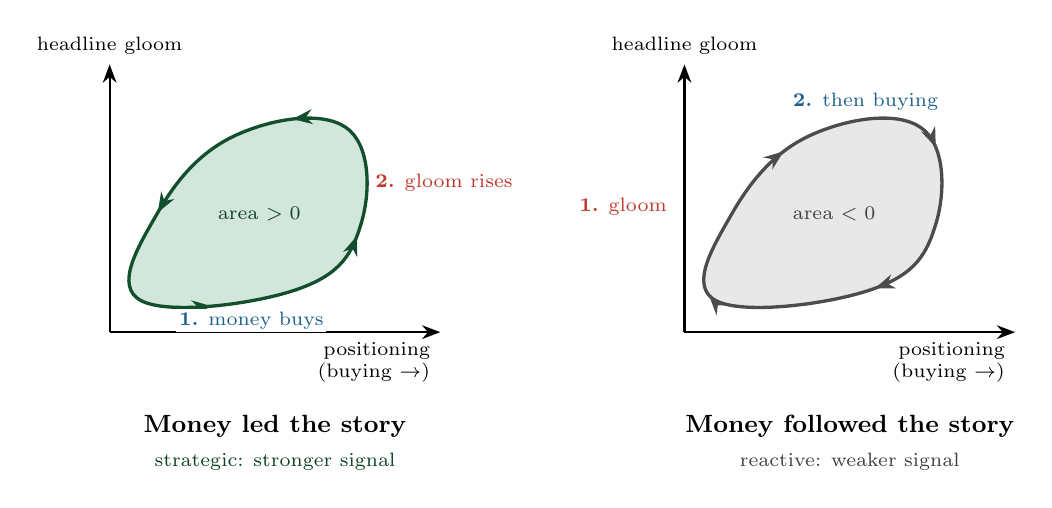
\begin{tikzpicture}[scale=1.0,
  arrowmid/.style={postaction={decorate}, decoration={markings,
    mark=at position 0.12 with {\arrow{Stealth[length=2.5mm]}},
    mark=at position 0.37 with {\arrow{Stealth[length=2.5mm]}},
    mark=at position 0.62 with {\arrow{Stealth[length=2.5mm]}},
    mark=at position 0.87 with {\arrow{Stealth[length=2.5mm]}}}}]
% left: money led
\begin{scope}
\draw[-{Stealth}, thick] (0,0) -- (4.2,0) node[below left, font=\scriptsize, align=right] {positioning\\(buying $\rightarrow$)};
\draw[-{Stealth}, thick] (0,0) -- (0,3.4) node[above, font=\scriptsize] {headline gloom};
\fill[good!20] plot[smooth cycle, tension=0.7] coordinates {(0.4,0.4) (2.4,0.55) (3.2,1.4) (3.0,2.6) (1.6,2.5) (0.6,1.5)};
\draw[good!60!black, very thick, arrowmid] plot[smooth cycle, tension=0.7] coordinates {(0.4,0.4) (2.4,0.55) (3.2,1.4) (3.0,2.6) (1.6,2.5) (0.6,1.5)};
\node[font=\scriptsize, text=good!50!black] at (1.9,1.5) {area $>0$};
\node[font=\scriptsize, anchor=north, text=do, fill=white, inner sep=1pt] at (1.8,0.3) {\textbf{1.} money buys};
\node[font=\scriptsize, anchor=west, text=echo] at (3.25,1.9) {\textbf{2.} gloom rises};
\node[font=\small\bfseries, align=center] at (2.1,-1.2) {Money led the story};
\node[font=\scriptsize, text=good!50!black] at (2.1,-1.65) {strategic: stronger signal};
\end{scope}
% right: money followed
\begin{scope}[xshift=7.3cm]
\draw[-{Stealth}, thick] (0,0) -- (4.2,0) node[below left, font=\scriptsize, align=right] {positioning\\(buying $\rightarrow$)};
\draw[-{Stealth}, thick] (0,0) -- (0,3.4) node[above, font=\scriptsize] {headline gloom};
\fill[gray!18] plot[smooth cycle, tension=0.7] coordinates {(0.4,0.4) (0.6,1.5) (1.6,2.5) (3.0,2.6) (3.2,1.4) (2.4,0.55)};
\draw[gray!60!black, very thick, arrowmid] plot[smooth cycle, tension=0.7] coordinates {(0.4,0.4) (0.6,1.5) (1.6,2.5) (3.0,2.6) (3.2,1.4) (2.4,0.55)};
\node[font=\scriptsize, text=gray!50!black] at (1.9,1.5) {area $<0$};
\node[font=\scriptsize, anchor=east, text=echo] at (-0.1,1.6) {\textbf{1.} gloom};
\node[font=\scriptsize, anchor=south, text=do] at (2.3,2.7) {\textbf{2.} then buying};
\node[font=\small\bfseries, align=center] at (2.1,-1.2) {Money followed the story};
\node[font=\scriptsize, text=gray!50!black] at (2.1,-1.65) {reactive: weaker signal};
\end{scope}
\end{tikzpicture}
\caption{\Cref{thm:levy,cor:lag}: the orientation of the loop in the (positioning, gloom) plane reveals who moved first, and its enclosed area (\cref{prop:levyprops}(iv)) measures how strongly.}
\label{fig:loop}
\end{figure}

% =====================================================================
\section{Regime Inference and Calibrated Uncertainty}\label{sec:inference}

Events belong to latent regimes $K_t\in\{\mathrm{I},\mathrm{O},\mathrm{S}\}$ (informational, overreaction, strategic) following a Markov chain, with emissions $\bm o_t\mid K_t=k\sim f_k$, where $\bm o_t$ collects $(s^{\text{new}},s^{\text{echo}},G,A,\mathcal{A},\dots)$.

\begin{proposition}[Causal filtering and mixture optimality]\label{prop:filter}
The filtered probabilities $\pi_t(k)=\Prob(K_t=k\mid\F_t)$ are $\F_t$-measurable and satisfy $\pi_t\propto f(\bm o_t)\odot P^\top\pi_{t-1}$. The MSE-optimal forecast is the mixture of experts
\[
  \E[r_{t+h}\mid\F_t]=\sum_k\pi_t(k)\,\E[r_{t+h}\mid\F_t,K_t=k].
\]
Smoothed probabilities $\Prob(K_t=k\mid\F_T)$, $T>t$, are not $\F_t$-measurable in general and must not be used for forecasting.
\end{proposition}
\begin{proof}
The recursion is Bayes' rule with prediction step $P^\top\pi_{t-1}$. The mixture follows from the tower property. Smoothed probabilities depend on $\bm o_{t+1:T}$.
\end{proof}

\begin{theorem}[Exponential detectability of strategic episodes]\label{thm:detect}
Consider an episode of $n$ events that are i.i.d.\ given a fixed regime, with $\bm o\sim\N(\bm m_0,\Sigma)$ under the null regime and $\N(\bm m_1,\Sigma)$ under the strategic regime, and priors $\pi_0,\pi_1$. The Bayes (MAP) misclassification probability satisfies
\[
  P_e\le\sqrt{\pi_0\pi_1}\;e^{-n\Delta^2/8}\le\tfrac12e^{-n\Delta^2/8},\qquad \Delta^2\coloneqq(\bm m_1-\bm m_0)^\top\Sigma^{-1}(\bm m_1-\bm m_0).
\]
Consequently $n\ge(8/\Delta^2)\log\big(1/(2\epsilon)\big)$ events suffice for $P_e\le\epsilon$.
\end{theorem}
\begin{proof}
$P_e=\int\min\{\pi_0p_0^{\otimes n},\pi_1p_1^{\otimes n}\}\le\sqrt{\pi_0\pi_1}\int\sqrt{p_0^{\otimes n}p_1^{\otimes n}}=\sqrt{\pi_0\pi_1}\,\mathrm{BC}^n$, using $\min\{a,b\}\le\sqrt{ab}$, where $\mathrm{BC}=\int\sqrt{p_0p_1}$ is the Bhattacharyya coefficient \citep{bhattacharyya1943,kailath1967}. For equal-covariance Gaussians, completing the square gives $\mathrm{BC}=e^{-\Delta^2/8}$ (\cref{lem:bc}). Finally $\sqrt{\pi_0\pi_1}\le\tfrac12$.
\end{proof}

\begin{figure}[ht]
\centering
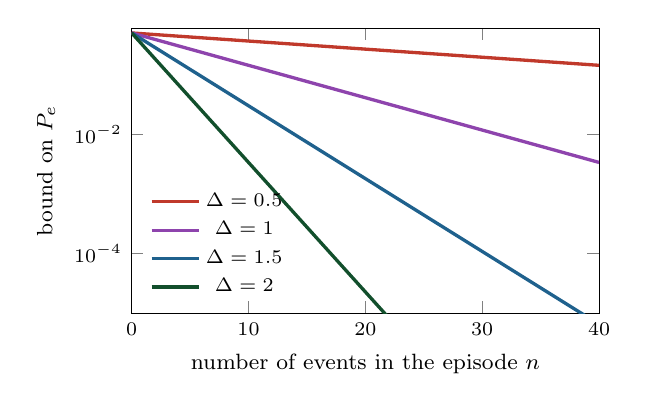
\begin{tikzpicture}
\begin{semilogyaxis}[width=0.62\textwidth, height=5.2cm, xmin=0, xmax=40, ymin=1e-5, ymax=0.6,
  xlabel={\footnotesize number of events in the episode $n$},
  ylabel={\footnotesize bound on $P_e$},
  legend style={font=\scriptsize, draw=none, fill=none, at={(0.02,0.02)}, anchor=south west},
  tick label style={font=\scriptsize}, samples=80, domain=0:40]
\addplot[echo, very thick] {0.5*exp(-x*0.25/8)}; \addlegendentry{$\Delta=0.5$}
\addplot[say, very thick] {0.5*exp(-x*1/8)}; \addlegendentry{$\Delta=1$}
\addplot[do, very thick] {0.5*exp(-x*2.25/8)}; \addlegendentry{$\Delta=1.5$}
\addplot[good!60!black, very thick] {0.5*exp(-x*4/8)}; \addlegendentry{$\Delta=2$}
\end{semilogyaxis}
\end{tikzpicture}
\caption{\Cref{thm:detect}. Detection error falls exponentially in the length of a strategic episode, at a rate set by the Mahalanobis separation $\Delta$ of the regime fingerprints.}
\label{fig:detect}
\end{figure}

Forecast intervals use adaptive conformal inference \citep{gibbs2021}. Let $\hat C_t(\alpha')$ be nested prediction sets with $\hat C_t(\alpha')=\R$ for $\alpha'\le0$ and $\hat C_t(\alpha')=\emptyset$ for $\alpha'\ge1$. Set $\mathrm{err}_t=\ind\{r_t\notin\hat C_t(\alpha_t)\}$ and $\alpha_{t+1}=\alpha_t+\gamma(\alpha-\mathrm{err}_t)$ with $\alpha_1\in[0,1]$ and $\gamma>0$.

\begin{theorem}[Deterministic long-run coverage; \citealp{gibbs2021}, Prop.~4.1]\label{thm:aci}
For \emph{every} sequence of outcomes, including adversarial or regime-switching ones,
\[
  \Big|\frac1T\sum_{t=1}^T\mathrm{err}_t-\alpha\Big|\le\frac{\max\{\alpha_1,1-\alpha_1\}+\gamma}{\gamma\,T}.
\]
\end{theorem}
\begin{proof}[Proof (reproduced for completeness)]
First, $\alpha_t\in[-\gamma,1+\gamma]$ for all $t$, by induction. If $\alpha_t<0$, then $\mathrm{err}_t=0$ and $\alpha_{t+1}=\alpha_t+\gamma\alpha\in(\alpha_t,\gamma\alpha)$. If $\alpha_t>1$, then $\mathrm{err}_t=1$ and $\alpha_{t+1}=\alpha_t-\gamma(1-\alpha)\in(1-\gamma(1-\alpha),\alpha_t)$. If $\alpha_t\in[0,1]$, then $\alpha_{t+1}\in[\alpha_t-\gamma(1-\alpha),\alpha_t+\gamma\alpha]$. In each case the interval lies in $[-\gamma,1+\gamma]$. Telescoping the update gives $\alpha_{T+1}-\alpha_1=\gamma\sum_{t\le T}(\alpha-\mathrm{err}_t)$, hence $|\frac1T\sum\mathrm{err}_t-\alpha|=|\alpha_{T+1}-\alpha_1|/(\gamma T)\le\max\{1+\gamma-\alpha_1,\alpha_1+\gamma\}/(\gamma T)$.
\end{proof}

% =====================================================================
\section{From Forecasts to Positions}\label{sec:sizing}

\begin{theorem}[Kelly shrinkage under estimation risk; classical, included for completeness]\label{thm:kelly}
Let an asset have excess drift $\mu$ and volatility $\sigma$, with continuous rebalancing at a constant fraction $f$, so that the long-run excess log-growth rate is $g(f)=f\mu-\tfrac12f^2\sigma^2$ \citep{merton1969}. Let $\hat\mu$ be an estimate with $\E\hat\mu=\mu$ and $\Var\hat\mu=s^2$, independent of future returns, and use $f=c\,\hat\mu/\sigma^2$. Then
\[
  \E\,g=\frac{c\mu^2-\tfrac12c^2(\mu^2+s^2)}{\sigma^2},\qquad
  c^\star=\frac{\mu^2}{\mu^2+s^2}=\frac{\mathrm{SNR}}{1+\mathrm{SNR}},\quad\mathrm{SNR}\coloneqq\frac{\mu^2}{s^2},
\]
with optimal growth $\mu^4/\big(2\sigma^2(\mu^2+s^2)\big)$. Full Kelly ($c=1$) yields $(\mu^2-s^2)/(2\sigma^2)$, which is negative whenever $s>|\mu|$.
\end{theorem}
\begin{proof}
$\E[f\mu]=c\mu^2/\sigma^2$ and $\E[f^2]\sigma^2/2=c^2(\mu^2+s^2)/(2\sigma^2)$. The resulting concave quadratic in $c$ is maximised at $c^\star$, and substitution gives the remaining expressions.
\end{proof}

\begin{figure}[ht]
\centering
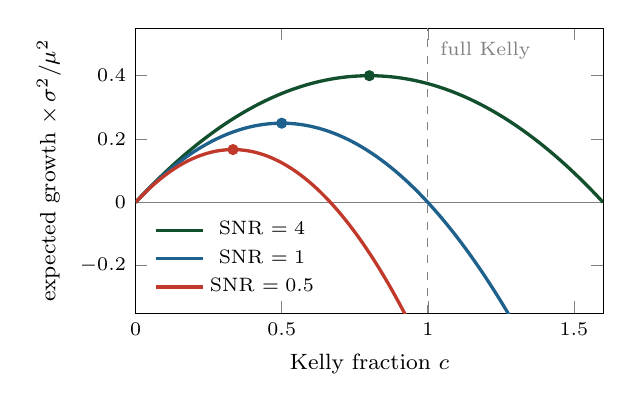
\begin{tikzpicture}
\begin{axis}[width=0.62\textwidth, height=5.2cm, xmin=0, xmax=1.6, ymin=-0.35, ymax=0.55,
  xlabel={\footnotesize Kelly fraction $c$},
  ylabel={\footnotesize expected growth $\times\,\sigma^2/\mu^2$},
  legend style={font=\scriptsize, draw=none, fill=none, at={(0.02,0.02)}, anchor=south west},
  tick label style={font=\scriptsize}, samples=100, domain=0:1.6]
\addplot[gray, thin, forget plot] coordinates {(0,0) (1.6,0)};
\addplot[good!60!black, very thick] {x - 0.5*x^2*(1+1/4)}; \addlegendentry{SNR $=4$}
\addplot[do, very thick] {x - 0.5*x^2*(1+1/1)}; \addlegendentry{SNR $=1$}
\addplot[echo, very thick] {x - 0.5*x^2*(1+1/0.5)}; \addlegendentry{SNR $=0.5$}
\addplot[only marks, mark=*, mark size=1.8pt, good!60!black, forget plot] coordinates {(0.8,0.4)};
\addplot[only marks, mark=*, mark size=1.8pt, do, forget plot] coordinates {(0.5,0.25)};
\addplot[only marks, mark=*, mark size=1.8pt, echo, forget plot] coordinates {(0.3333,0.16667)};
\addplot[dashed, gray, forget plot] coordinates {(1,-0.35) (1,0.55)};
\node[font=\scriptsize, text=gray, anchor=south west] at (axis cs:1.01,0.42) {full Kelly};
\end{axis}
\end{tikzpicture}
\caption{\Cref{thm:kelly}. Expected growth as a function of the Kelly fraction for three signal-to-noise ratios; dots mark $c^\star=\mathrm{SNR}/(1+\mathrm{SNR})$. With noisy edge estimates, full Kelly destroys growth. The conformal interval width of \cref{thm:aci} supplies $s$.}
\label{fig:kelly}
\end{figure}

\begin{proposition}[Well-posed portfolio construction]\label{prop:convex}
For $\hat\Sigma\succ0$, risk aversion $\gamma_r>0$, cost coefficients $c_i,\eta_i\ge0$, factor exposures $B$ and bounds $\bar w,G>0$, the programme
\begin{align*}
  \max_{\w}\quad & \bm\alpha^\top\w-\tfrac{\gamma_r}{2}\w^\top\hat\Sigma\w-\sum_ic_i|w_i-w_i^0|-\sum_i\eta_i\sigma_i\frac{|w_i-w_i^0|^{3/2}}{\sqrt{V_i}}\\
  \text{s.t.}\quad & B^\top\w=\bm 0,\quad \bm 1^\top\w=0,\quad |w_i|\le\bar w,\quad \|\w\|_1\le G
\end{align*}
has a unique solution. The $3/2$-power term integrates square-root impact \citep{bouchaud2018}.
\end{proposition}
\begin{proof}
The feasible set is a nonempty ($\w=\bm 0$ is feasible), compact and convex polytope. The objective is continuous and strictly concave: it is a linear term, minus a strictly convex quadratic, minus convex functions $|\cdot|$ and $|\cdot|^{3/2}$. A continuous function attains its maximum on a compact set, and strict concavity makes the maximiser unique.
\end{proof}

% =====================================================================
\section{Synthesis}\label{sec:synthesis}

Every component of the composite score has a sign dictated by a theorem:
\[
  D_{i,t}=
  \underbrace{\omega_1\,s^{\text{new}}}_{\substack{\text{follow news}\\ \text{Cor.~\ref{cor:news}}}}
  \;-\;\underbrace{\omega_2\,s^{\text{echo}}}_{\substack{\text{fade echo}\\ \text{Cor.~\ref{cor:echo}}}}
  \;+\;\underbrace{\omega_3\,\text{Do}}_{\substack{\text{follow deeds}\\ \text{Thm.~\ref{thm:identity}}}}
  \;+\;\underbrace{\widehat{\sgn}\,\omega_4\gamma\,\text{Say}}_{\substack{\text{follow or fade words}\\ \text{Thm.~\ref{thm:identity}}}}
  \;+\;\underbrace{\omega_5\,A}_{\substack{\text{absorption}\\ \text{Thm.~\ref{thm:absorption}}}}
  \;+\;\underbrace{\omega_6\,\mathcal{A}^{\pm}}_{\substack{\text{money led}\\ \text{Thm.~\ref{thm:levy}}}},
\]
where $\widehat{\sgn}$ is the sign of the rolling estimate of $\Cov(\text{Say},\text{Do})$ and $\mathcal{A}^{\pm}$ is the L\'evy area signed by the direction of the positioning change. By \cref{thm:identity}, deeds are always followed, while words are followed when the covariance is positive and faded when it is negative. In the second case, and with $\omega_3=\omega_4$, the two terms combine into $-\omega_3G_\gamma$, the Say--Do gap of \cref{thm:saydo}. By \cref{thm:cycles}, the sign may alternate from period to period. A fitted weight with the wrong sign is a diagnostic that the model's assumptions fail in that market. In the full system, $D$ is replaced by the regime mixture of \cref{prop:filter}, wrapped in the intervals of \cref{thm:aci}, and sized by \cref{thm:kelly} (\cref{fig:pipeline}).

\begin{figure}[ht]
\centering
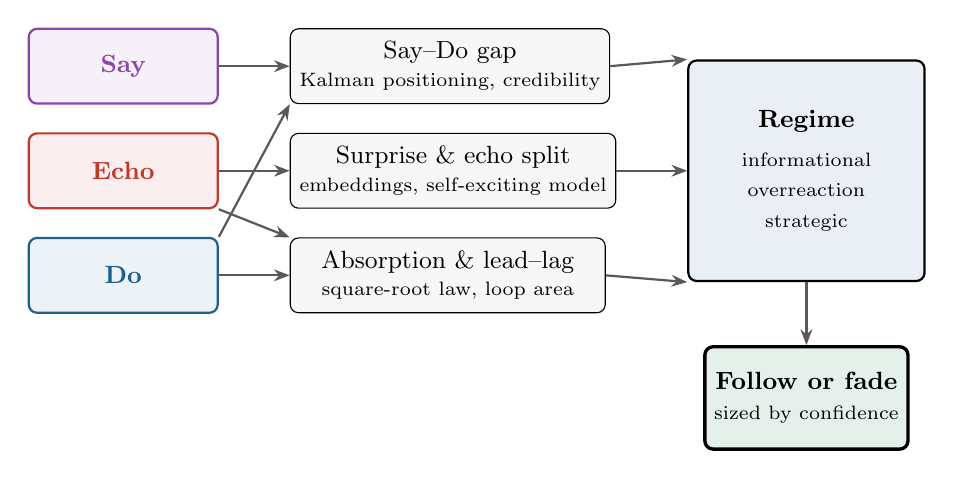
\begin{tikzpicture}[
  node distance=0.35cm and 0.9cm,
  voice/.style={draw, rounded corners=3pt, thick, minimum width=2.4cm, minimum height=0.95cm, align=center, font=\small\bfseries},
  sig/.style={draw, rounded corners=3pt, fill=gray!6, minimum width=4.0cm, minimum height=0.95cm, align=center, font=\small},
  arr/.style={-{Stealth[length=2mm]}, thick, gray!70!black}]
\node[voice, draw=say, fill=say!8, text=say] (say) {Say};
\node[voice, draw=echo, fill=echo!8, text=echo, below=of say] (echo) {Echo};
\node[voice, draw=do, fill=do!8, text=do, below=of echo] (do) {Do};
\node[sig, right=of say] (gap) {Say--Do gap\\[-1pt]\scriptsize Kalman positioning, credibility};
\node[sig, right=of echo] (news) {Surprise \& echo split\\[-1pt]\scriptsize embeddings, self-exciting model};
\node[sig, right=of do] (abs) {Absorption \& lead--lag\\[-1pt]\scriptsize square-root law, loop area};
\node[draw, rounded corners=3pt, thick, fill=do!10, minimum width=3.0cm, minimum height=2.8cm, align=center, font=\small, right=of news] (reg) {\textbf{Regime}\\[3pt]\scriptsize informational\\\scriptsize overreaction\\\scriptsize strategic};
\node[draw, rounded corners=3pt, very thick, fill=good!12, minimum width=2.4cm, minimum height=1.3cm, align=center, font=\small, below=0.8cm of reg] (dec) {\textbf{Follow or fade}\\\scriptsize sized by confidence};
\draw[arr] (say) -- (gap);
\draw[arr] (do.north east) -- (gap.south west);
\draw[arr] (echo) -- (news);
\draw[arr] (echo.south east) -- (abs.north west);
\draw[arr] (do) -- (abs);
\draw[arr] (gap.east) -- (reg.north west);
\draw[arr] (news) -- (reg);
\draw[arr] (abs.east) -- (reg.south west);
\draw[arr] (reg) -- (dec);
\end{tikzpicture}
\caption{The complete architecture: three voices, three families of signals, one regime-aware decision.}
\label{fig:pipeline}
\end{figure}

\begin{tcolorbox}[enhanced,breakable,colback=gray!4,colframe=gray!55!black,boxrule=0.6pt,arc=2pt,
  fonttitle=\bfseries\small,title={Illustration: a hypothetical downgrade (numbers are illustrative, not data)},left=8pt,right=8pt]
\small
\textbf{Before.} Over eight days, call open interest rises, put skew flattens, and two directors buy shares. \textbf{Day 0.} Two brokers downgrade the stock, and coverage jumps from 15 to 140 articles a day.

\begin{tabularx}{\linewidth}{@{}Xr@{}}
\toprule
Quantity (result used) & Reading \\
\midrule
News / echo sentiment (\cref{prop:mmse}) & $-0.5\sigma$ / $-2.3\sigma$ \\
Branching ratio, i.e.\ echo share (\cref{prop:branching}) & 0.82 \\
Say--Do gap (\cref{thm:saydo}) & bearish words, bullish positioning \\
Say--Do covariance (\cref{thm:identity}) & negative: fade the words \\
Expected vs actual reaction, absorption (\cref{prop:analog,thm:absorption}) & $-6.0\%$ vs $-1.9\%$; $A=+1.6$ \\
L\'evy area rate (\cref{thm:levy}) & positive: money moved first \\
Regime posterior I / O / S (\cref{prop:filter}) & 0.10 / 0.28 / 0.62 \\
Kelly fraction (\cref{thm:kelly}) with SNR $\approx0.5$ & $c^\star\approx0.33$ \\
\bottomrule
\end{tabularx}

\textbf{Reading.} A probable false alarm: lean long, sized at about a third of full Kelly.
\end{tcolorbox}

% =====================================================================
\section{Numerical Verification}\label{sec:verify}

Every closed form in this paper was checked against an independent computation (\cref{tab:verify}). Theory values are exact functions of the model parameters. The Gaussian results of \cref{sec:model} were checked by regression on $2\times10^6$ simulated draws. \Cref{thm:identity} was checked with fat-tailed values ($t_3$) and Laplace message noise, which tests its distribution-free claim. Optimal speech was compared with numerical optimisation, \cref{thm:semantic} with brute-force enumeration of every parent labelling, and \cref{thm:levy} with a smooth Gaussian process with a known lag. Both forms of \cref{thm:robustnn} were checked on $3{,}000$ random pairs of target and model distributions: no certified pair was ever misordered, and the exact form certified $3.6$ times as many pairs as the Pinsker form (the ratio depends on how instances are drawn; see \texttt{scripts/check\_certificate.py}). The $t_3$ exaggeration case converges most slowly because the fourth moment of a $t_3$ variable is infinite; the pathwise identity $r=\lambda x-\varphi\varepsilon$ itself holds to machine precision.

\begin{table}[ht]
\centering
\caption{Theory versus independent checks ($2\times10^6$ draws, seed 0).}
\label{tab:verify}
\small
\begin{tabularx}{0.94\textwidth}{@{}l>{\raggedright\arraybackslash}Xrr@{}}
\toprule
Result & Quantity & Theory & Check \\
\midrule
\multicolumn{4}{@{}l}{\footnotesize\color{gray} Three-voice economy (\cref{sec:model})}\\
\cref{cor:echo} & Bayes weight on the echo channel & $0$ & $-0.0006$ \\
\cref{thm:followfade} & return loading on the echo channel & $-0.1840$ & $-0.1843$ \\
\cref{thm:saydo} & loading on positioning, $c_x$ & $0.4012$ & $0.4004$ \\
\cref{thm:absorption} & absorption coefficient, $c_A$ & $-0.1997$ & $-0.2004$ \\
\multicolumn{4}{@{}l}{\footnotesize\color{gray} Strategic speech (\cref{sec:strategic})}\\
\cref{thm:speech} & speech slope $\psi$ ($\varphi=0.6$, $a=0.5$) & $-0.7143$ & $-0.7143$ \\
\cref{thm:speech} & trade slope $\chi$ ($\varphi=0.6$, $a=0.5$) & $1.4286$ & $1.4286$ \\
\cref{thm:identity} & $\Cov(r,\text{Say})$, $t_3$ values, false alarm & $-2.294$ & $-2.293$ \\
\cref{thm:identity} & $\Cov(r,\text{Say})$, $t_3$ values, exaggeration & $-7.608$ & $-7.676$ \\
\cref{thm:cycles} & 2-cycle points at $a=1.95$ & $\{0.8189,\,1.1311\}$ & $\{0.8189,\,1.1311\}$ \\
\cref{thm:cycles} & 2-cycle multiplier at $a=1.8$ & $0$ & $9\times10^{-16}$ \\
\multicolumn{4}{@{}l}{\footnotesize\color{gray} Measurement (\cref{sec:echo,sec:embeddings,sec:leadlag})}\\
\cref{thm:semantic} & largest error of the factorised posterior & $0$ & $1.1\times10^{-16}$ \\
\cref{thm:levy} & L\'evy-area rate, lag $0.5$ & $0.2356$ & $0.2360$ \\
\cref{thm:robustnn} & wrongly ordered certified pairs, $3{,}000$ random cases & $0$ & $0$ \\
\multicolumn{4}{@{}l}{\footnotesize\color{gray} Sizing (\cref{sec:sizing})}\\
\cref{thm:kelly} & growth at the shrunk Kelly fraction $c^\star$ & $0.01056$ & $0.01055$ \\
\cref{thm:kelly} & growth at full Kelly & $-0.0300$ & $-0.0300$ \\
\bottomrule
\end{tabularx}
\end{table}

Exactness does not by itself show that meaning \emph{helps}. We therefore simulated cascades in which each echo is a von Mises--Fisher copy of its parent with concentration $\varkappa$ (\cref{ass:marked}; Hawkes $\mu=0.6$, $\alpha=1$, $\beta=1.25$; $16$-dimensional embeddings; about $2{,}000$--$2{,}800$ articles per run) and asked each method to recover the true parent of every article. Timing alone recovers about one parent in four at every concentration. Adding meaning raises accuracy to $95\%$ when echoes are close copies, and it nearly eliminates the error in each article's probability of being an echo (\cref{fig:decluster}).

\begin{figure}[ht]
\centering
\begin{minipage}{0.48\textwidth}
\centering
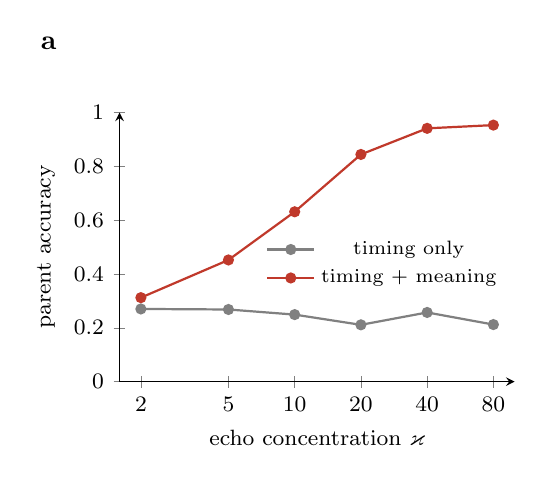
\begin{tikzpicture}
\begin{semilogxaxis}[width=6.6cm, height=5.0cm, xmin=1.6, xmax=100, ymin=0, ymax=1,
  xtick={2,5,10,20,40,80}, xticklabels={2,5,10,20,40,80}, log ticks with fixed point,
  xlabel={\footnotesize echo concentration $\varkappa$}, ylabel={\footnotesize parent accuracy},
  tick label style={font=\footnotesize}, axis lines=left,
  legend style={font=\scriptsize, draw=none, fill=none, at={(0.99,0.31)}, anchor=south east}]
\addplot[gray, thick, mark=*, mark size=1.6pt] coordinates {(2,0.270) (5,0.268) (10,0.249) (20,0.211) (40,0.257) (80,0.212)};
\addlegendentry{timing only}
\addplot[echo, thick, mark=*, mark size=1.6pt] coordinates {(2,0.312) (5,0.452) (10,0.631) (20,0.844) (40,0.941) (80,0.953)};
\addlegendentry{timing + meaning}
\end{semilogxaxis}
\node[font=\bfseries] at (-0.9,4.3) {a};
\end{tikzpicture}
\end{minipage}\hfill
\begin{minipage}{0.48\textwidth}
\centering
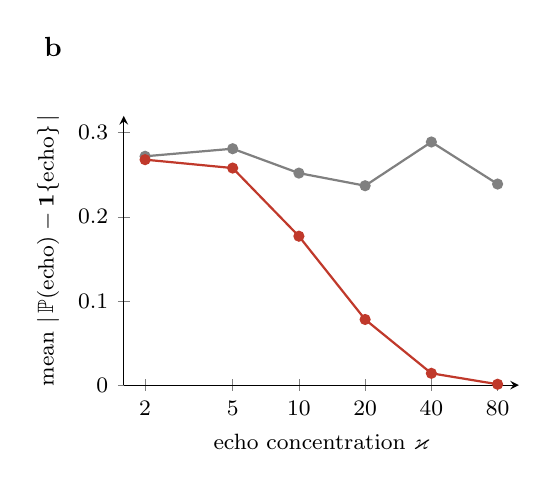
\begin{tikzpicture}
\begin{semilogxaxis}[width=6.6cm, height=5.0cm, xmin=1.6, xmax=100, ymin=0, ymax=0.32,
  xtick={2,5,10,20,40,80}, xticklabels={2,5,10,20,40,80},
  ytick={0,0.1,0.2,0.3}, yticklabels={0,0.1,0.2,0.3},
  xlabel={\footnotesize echo concentration $\varkappa$}, ylabel={\footnotesize mean $|\,\Prob(\text{echo})-\ind\{\text{echo}\}\,|$},
  tick label style={font=\footnotesize}, axis lines=left]
\addplot[gray, thick, mark=*, mark size=1.6pt] coordinates {(2,0.272) (5,0.281) (10,0.252) (20,0.237) (40,0.289) (80,0.239)};
\addplot[echo, thick, mark=*, mark size=1.6pt] coordinates {(2,0.268) (5,0.258) (10,0.177) (20,0.078) (40,0.014) (80,0.001)};
\end{semilogxaxis}
\node[font=\bfseries] at (-0.9,4.3) {b};
\end{tikzpicture}
\end{minipage}
\caption{Meaning makes echo detection work (\cref{thm:semantic}). \textbf{a}: accuracy of the most likely parent. \textbf{b}: mean absolute error of each article's echo probability. Grey: timing only ($\varkappa=0$ in the posterior). Red: timing and meaning.}
\label{fig:decluster}
\end{figure}

% =====================================================================
\section{Controlled Experiments}\label{sec:experiments}

The checks in \cref{sec:verify} show that the formulas are right. They do not show that the tools work once parameters have to be estimated, the model is only approximately true, and the signal is buried in noise. Before going to market data we therefore built a simulated market in which the truth is known, gave every method only what an econometrician would see, and asked five questions.
\begin{enumerate}[label=\textbf{Q\arabic*.}, leftmargin=2.2em]
  \item Can repetition be separated from news, and do the two move returns in opposite directions?
  \item Does the Say--Do covariance identify the institutions whose words should be faded?
  \item Do absorption and lead--lag carry the signs the theory predicts?
  \item Do features built from the theory improve forecasts over strong baselines?
  \item Do return-aligned embeddings organise text by consequence, and is the certificate informative?
\end{enumerate}
Some answers are yes, some are ``only partly'', and one is no. We report all of them.

\subsection{Design}

\paragraph{The market.} There are $300$ firms and $60$ events per firm. Each firm hosts one institution whose parameters are fixed across events. A quarter of the institutions are non-strategic: they report value and do not trade. The rest are strategic, with credulity $\varphi$ and deterrence $a=2\lambda k$ drawn inside the shading, false-alarm or exaggeration region of \cref{cor:taxonomy}. Each firm's regime is drawn with probability one quarter for each of the four. At each event:
\begin{enumerate}[label=(\arabic*)]
  \item value is drawn, $v\sim\N(0,1)$;
  \item the institution trades $x=\chi v$, spread evenly over the ten days before it speaks, and then publishes $\text{Say}=\psi v+\N(0,0.3^2)$, with $(\psi,\chi)$ from \cref{thm:speech};
  \item the media publish a Hawkes cascade over the next ten days. The statement is the first article. Independent news items arrive at rate $0.4$ per day, each carrying the sentiment $v+\N(0,1.5^2)$. Every article can be echoed, with branching ratio $n=1-\varphi_0/\varphi$ so that the crowd's effective credulity is $\varphi$ (\cref{prop:virality}). Echoes arrive after exponential delays with rate $1.5$, copy their parent's sentiment up to noise $\N(0,0.15^2)$, and copy its $16$-dimensional embedding up to a von Mises--Fisher perturbation with $\varkappa=30$ (\cref{ass:marked});
  \item the crowd prices every article, $p=\sum_j w_j s_j+\lambda(x+u)$, where $w_j=\varphi_0$ for the statement and its echoes, $w_j=0.04$ for news and its echoes, and $u\sim\N(0,0.4^2)$ is noise trading;
  \item the forward return is $r=v-p+\eta$, where $\eta\sim\N(0,10^2)$ is information that arrives later, and positioning is revealed with error, $\text{Do}=x+\N(0,0.5^2)$.
\end{enumerate}

\paragraph{What the methods see.} Every method sees the article times, embeddings and sentiment scores, the statement, the noisy positioning, the price reaction, and daily paths of positioning and cumulative tone from ten days before the statement to ten days after it. No forecasting method sees value, regimes, parentage or any model parameter. The one exception is the false-alarm detector of Q2, which is trained on the true regime labels of the training half, as a supervised detector would be on labelled historical episodes.

\paragraph{Protocol.} The first $30$ events of each firm form the training set and the last $30$ the test set. Every estimated quantity uses the training half only. This includes the Hawkes parameters (pooled maximum likelihood), the echo concentration $\varkappa$ (marked likelihood), the narrative-implied price move, all regression and boosting weights, and all standardisations. The features of an event use only that event's articles and price reaction and the firm's earlier events. \Cref{tab:features} lists the features.

\begin{table}[ht]
\centering
\caption{Features built from the theory. All are computed causally.}
\label{tab:features}
\small
\begin{tabularx}{\textwidth}{@{}l>{\raggedright\arraybackslash}Xl@{}}
\toprule
Feature & Construction & Source \\
\midrule
News, echo & $s^{\text{new}}=\sum_j\Prob(\text{news}_j)\,s_j$ over articles other than the statement; $s^{\text{echo}}=\sum_j\Prob(\text{echo}_j)\,s_j$ & \cref{prop:mmse,thm:semantic} \\
Say--Do switch & correlation of Say and Do over the firm's previous $20$ events; words are faded when it is below $-0.2$ & \cref{thm:identity} \\
Absorption & price reaction minus the narrative-implied move, fitted linearly on Say, $s^{\text{new}}$ and $s^{\text{echo}}$ (pooled, or per firm; tone is their sum) & \cref{thm:absorption} \\
Lead--lag & L\'evy area of (positioning, $-$tone) over the event window, signed by the direction of the positioning change & \cref{thm:levy} \\
Composite & unit weights on the standardised terms above, with the switch applied to Say & \cref{sec:synthesis} \\
\bottomrule
\end{tabularx}
\end{table}

\paragraph{Calibration, and what we changed.} The features, tests and strategies were fixed before we looked at any of their results. The simulator's scale was then calibrated as follows. A pilot run exposed two degenerate properties of the raw simulator: prices moved about $3.3$ times as much as fundamentals, and fading the tone alone reached an information coefficient of $0.89$. We lowered the per-article impact of news from $0.12$ to $0.04$ and restricted the credulity of non-strategic institutions to $(0.4,0.95)$. We then chose the scale of the late information $\eta$ so that a linear regression on the raw voices, which uses no theory at all, reaches an out-of-sample information coefficient of about $0.17$. That is far more predictable than any real market. We chose it so that differences between methods are visible with $300$ firms, and only comparisons between methods should be read from the results. The calibration also caps what any method can achieve. Forecasting with the true mispricing $v-p$ gives an IC of $0.181$ (between $0.165$ and $0.206$ across seeds), only about $0.01$ above the linear baseline.

\paragraph{Metrics.} For forecasts we report the cross-sectional information coefficient (IC) in each of the $30$ test periods, its average and its $t$-statistic across periods, and the per-period Sharpe ratio of a dollar-neutral portfolio with weights proportional to the standardised score. The theory tests are pooled regressions of test-period returns on standardised features, with standard errors clustered by firm. The main market is simulated with five seeds, every robustness variant with three, and every sample size with two. Together these give $29$ distinct simulated markets. The ``timing only'' variant re-analyses three of them, so there are $32$ analyses in all.

\subsection{Results}

\paragraph{Q1: repetition can be separated from news, and fading it works.} The semantic declustering step recovers the echo concentration almost exactly ($\hat\varkappa=30.27\pm0.07$ against a true $30$) and the share of articles that are echoes ($0.422$ against $0.427$). On the same simulated markets, declustering by timing alone estimates an echo share of $0.368$ against a true $0.430$, because it mistakes many echoes for news. The prediction of \cref{cor:echo} holds without exception. Echo sentiment predicts returns with a significantly negative sign in every one of the $29$ simulated markets, with a mean $t$-statistic of $-8.0$ in the main market (\cref{tab:tests}). Meaning sharpens the test: on identical markets, the $t$-statistic weakens from $-7.5$ to $-6.0$ when timing alone is used. The news prediction of \cref{cor:news} also holds, but more weakly. The sign is positive in every market, the mean $t$-statistic is $+2.1$, and the effect is significant in $21$ of the $29$ markets. News is harder to detect because each news article is a noisy signal of value and the crowd underreacts to it only modestly.

\begin{table}[ht]
\centering
\caption{Theory tests on the test half of the main market (five seeds). Coefficients are in units of fundamental value per training standard deviation of the feature. $t$: firm-clustered, averaged over seeds. The last column counts seeds with $|t|>2$ and the predicted sign.}
\label{tab:tests}
\small
\begin{tabularx}{\textwidth}{@{}>{\raggedright\arraybackslash}Xlrrc@{}}
\toprule
Regressor (controls) & Prediction & Coef. & $t$ & As predicted \\
\midrule
News sentiment $s^{\text{new}}$ (Say, Do) & $+$ \ (\cref{cor:news}) & $+0.35$ & $+2.1$ & 3/5 \\
Echo sentiment $s^{\text{echo}}$ (Say, Do) & $-$ \ (\cref{cor:echo}) & $-1.52$ & $-8.0$ & 5/5 \\
\addlinespace
Say, fade group (Do) & $-$ \ (\cref{thm:identity}) & & $-3.3$ & 4/5 \\
Say, fade group (Do, news, echo) & $-$ & $-0.06$ & $-0.3$ & 1/5 \\
Say, follow group (Do, news, echo) & either & $+0.10$ & $+0.4$ & -- \\
Do (Say by group, news, echo) & $+$ & $+0.14$ & $+0.9$ & 1/5 \\
\addlinespace
Absorption, all events & either \ (\cref{thm:absorption}) & $-1.27$ & $-11.6$ & -- \\
\quad institution does not trade & $-$ & $-1.25$ & $-3.6$ & 4/5 \\
\quad institution trades & either & $-1.27$ & $-11.1$ & -- \\
Absorption, firm-level multiplier & either & $-0.72$ & $-9.0$ & -- \\
\quad institution does not trade & $-$ & $-1.03$ & $-4.0$ & 5/5 \\
\addlinespace
Signed L\'evy area & $+$ \ (\cref{thm:levy}) & $+0.23$ & $+1.0$ & 1/5 \\
\bottomrule
\end{tabularx}
\end{table}

\paragraph{Q2: the Say--Do covariance finds the institutions whose words should be faded.} On its own, the rolling correlation between Say and Do separates the events of false-alarm institutions from all others with an AUC of $0.895$ (\cref{fig:falsealarms}b). A logistic classifier that adds four other observable features, trained on the true labels of the training half, reaches $0.934\pm0.010$ on later events of the same firms. Real data would supply such labels only through episodes identified after the fact. The single-feature AUCs are reported as $\max(\text{AUC},1-\text{AUC})$, so the values near $0.5$ for absorption and echo share mean ``uninformative''. Used as the switch of \cref{sec:synthesis}, the same correlation labels correctly whether a firm's words should be faded (false-alarm and exaggerating institutions, the two regimes in which $\Cov(\text{Say},\text{Do})<0$) $85\%$ of the time from five past events and $96\%$ of the time from forty (\cref{fig:falsealarms}a). In the group it flags, statements predict returns with the sign reversed: the average $t$-statistic is between $-3.0$ and $-3.3$ at every window length, and it is significant in four of five seeds. In the other group the average $t$-statistic is between $-0.6$ and $-1.0$. We report that sign as an empirical finding. The identity does not cover non-strategic institutions, whose silence in the market is not optimal given the crowd's credulity.

Two caveats matter for real data. First, once news and echo sentiment are added as controls, the reversed coefficient on Say in the flagged group is no longer significant ($t=-0.3$). Echo sentiment alone is enough to remove it ($t=+0.2$ on average), while news alone only weakens it ($t=-2.0$). In this market most of a statement's price impact travels through its echoes, so the echo control absorbs it. Second, Do's own coefficient is imprecise, for two reasons. With Say, news and echo all controlled its $t$-statistic is $+0.9$, partly because Say and Do are nearly collinear within the strategic regimes (their correlation is $-0.87$ for false alarms, $-0.78$ for exaggeration and $+0.54$ for shading), so a regression cannot divide credit between them. Even with Say removed, the $t$-statistic averages only $+1.6$, because the institution's price impact is small next to the information that arrives later. The collinearity is also why \cref{thm:saydo} works with the gap between the two voices rather than with either voice alone.

\begin{figure}[ht]
\centering
\begin{minipage}[t]{0.46\textwidth}
\centering
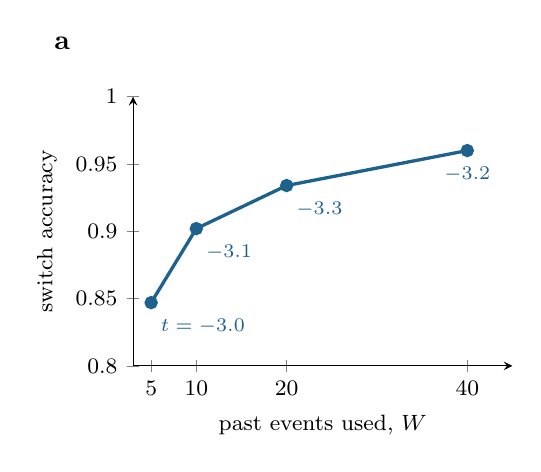
\begin{tikzpicture}
\begin{axis}[width=6.4cm, height=5.0cm, xmin=3, xmax=45, ymin=0.8, ymax=1.0,
  xtick={5,10,20,40}, ytick={0.8,0.85,0.9,0.95,1.0},
  yticklabel style={/pgf/number format/fixed, /pgf/number format/precision=2},
  xlabel={\footnotesize past events used, $W$}, ylabel={\footnotesize switch accuracy},
  tick label style={font=\footnotesize}, axis lines=left, clip=false]
\addplot[do, very thick, mark=*, mark size=1.8pt] coordinates {(5,0.847) (10,0.902) (20,0.934) (40,0.960)};
\node[font=\scriptsize, anchor=north west, text=do] at (axis cs:5,0.842) {$t=-3.0$};
\node[font=\scriptsize, anchor=north west, text=do] at (axis cs:10,0.897) {$-3.1$};
\node[font=\scriptsize, anchor=north west, text=do] at (axis cs:20,0.929) {$-3.3$};
\node[font=\scriptsize, anchor=north, text=do] at (axis cs:40,0.955) {$-3.2$};
\end{axis}
\node[font=\bfseries] at (-0.9,4.1) {a};
\end{tikzpicture}
\end{minipage}\hfill
\begin{minipage}[t]{0.50\textwidth}
\centering
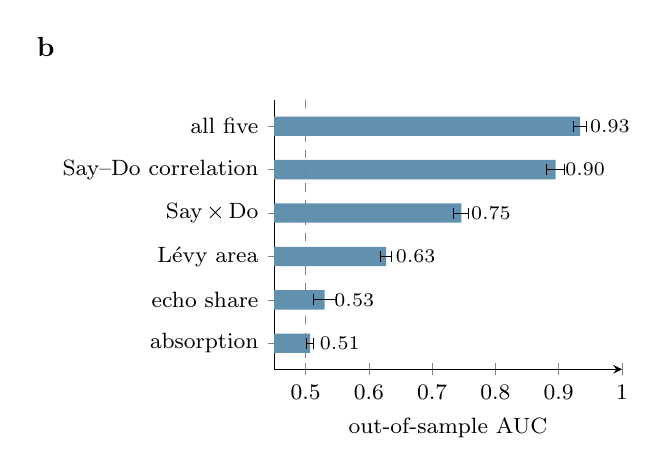
\begin{tikzpicture}
\begin{axis}[xbar, width=6.0cm, height=5.0cm, xmin=0.45, xmax=1.0, bar width=7pt,
  ytick={1,...,6}, y dir=reverse, ymin=0.4, ymax=6.6,
  yticklabels={all five, Say--Do correlation, Say$\,\times\,$Do, L\'evy area, echo share, absorption},
  xtick={0.5,0.6,0.7,0.8,0.9,1.0}, xlabel={\footnotesize out-of-sample AUC},
  tick label style={font=\footnotesize}, axis lines=left,
  xticklabel style={/pgf/number format/fixed, /pgf/number format/precision=1},
  y axis line style={-}, nodes near coords, nodes near coords style={font=\scriptsize, /pgf/number format/fixed, /pgf/number format/zerofill, /pgf/number format/precision=2}]
\addplot[fill=do!70, draw=none, error bars/.cd, x dir=both, x explicit] coordinates {(0.934,1) +- (0.010,0) (0.895,2) +- (0.014,0) (0.746,3) +- (0.012,0) (0.627,4) +- (0.009,0) (0.530,5) +- (0.018,0) (0.507,6) +- (0.006,0)};
\draw[gray, dashed] (axis cs:0.5,0.4) -- (axis cs:0.5,6.6);
\end{axis}
\node[font=\bfseries] at (-2.9,4.1) {b};
\end{tikzpicture}
\end{minipage}
\caption{Finding the false alarms. \textbf{a}: how often the rolling Say--Do correlation correctly labels a firm's words as ones to fade, against the number of past events used. Labels give the $t$-statistic of statements in the flagged group, which is negative as \cref{thm:identity} predicts. \textbf{b}: AUC for flagging the events of false-alarm institutions, for each feature alone and for a logistic classifier on all five trained with true labels (mean $\pm$ s.d.\ over five seeds; dashed: chance).}
\label{fig:falsealarms}
\end{figure}

\paragraph{Q3: absorption measures the narrative model as much as the market; lead--lag is weak.} Absorption predicts strong \emph{reversal} ($t=-11.6$), and it does so in all $29$ markets. It does so both where institutions trade, where \cref{thm:absorption} allows either sign, and where they do not ($t=-3.6$), where it predicts reversal. The second result looks like a confirmation, but it is not, and \texttt{experiments/diagnostics.py} shows why.

Absorption is the residual of the price reaction after the narrative-implied move has been removed. Here only $12$--$19\%$ of the residual's variance is the institution's trade and $2$--$4\%$ is noise trading. Almost all of the rest is \emph{narrative misfit}, the part of the crowd's reaction that a linear narrative model fails to capture. The misfit has a simple source. The statement's price impact is multiplied by the size of its echo cascade, and $s^{\text{echo}}$ pools the statement's echoes, which the crowd weights heavily, with the more numerous echoes of news, which it weights lightly. Adding Say times cascade size to the narrative model weakens the reversal from $t\approx-12$ to $t\approx-3.5$ on average. If we replace the estimate with the true absorption $\lambda(x+u)$, which a perfect narrative model would recover, the coefficient is insignificant in both groups: $t$ ranges from $-1.2$ to $+0.5$ where institutions trade and from $-1.4$ to $+0.8$ where they do not. \Cref{lem:robust} protects absorption against a wrong multiplier. It does not protect it against a price that is not linear in the channels the model uses.

Our experiments therefore neither confirm nor refute \cref{thm:absorption}: the simulated trades are too small relative to later information to reveal either sign. What they do show is practical. The sign of estimated absorption depends on the narrative model and must be estimated, never assumed. In the unit-weight composite, the absorption term enters with the wrong sign for this market, and removing it doubles the composite's IC from $0.049$ to $0.096$.

The signed L\'evy area has the predicted positive sign in $27$ of the $29$ markets, but it is significant in only $9$ ($t=+1.0$ in the main market). It is more useful for detecting false alarms (AUC $0.63$) than for predicting returns.

\paragraph{Q4: the theory adds little forecasting power, but there was little to add.} \Cref{fig:ic} ranks twelve forecasts. Following the tone loses money. Following institutional statements loses money too, because half of the institutions are in regimes whose words should be faded, and even the others' statements are already priced through their echoes. Fading the price reaction is a strong baseline (IC $0.162$). A linear regression on the raw voices does slightly better ($0.169$). Adding the theory's features to that regression changes almost nothing ($0.171$, at most about $0.005$ better in any seed). For gradient boosting the features help a little: $0.109$ becomes $0.118$ in the main market, and the features improve boosting by more than $0.001$ in $18$ of the $29$ markets. The unit-weight composite of \cref{sec:synthesis} is weak ($0.049$), mostly because of the absorption term discussed above.

This comparison has little power, and we do not read much into it. Forecasting with the true mispricing $v-p$, which no method can observe, reaches only $0.181$, so there is about $0.01$ of IC between the linear baseline and perfection. With so little room, the result is consistent with the theory adding nothing and also with it adding a great deal of what is left. Two points are nonetheless clear. First, \cref{thm:followfade} says the optimal forecast is linear in the voices, and a regression free to learn the weights comes close to the ceiling, as that theorem suggests. Second, the unit-weight composite is not a good trading rule; the composite of \cref{sec:synthesis} should be used with fitted weights. The theory's clearest contributions in these experiments are the signs it predicts and the diagnostics of Q1 and Q2, not extra forecasting power.

\begin{figure}[ht]
\centering
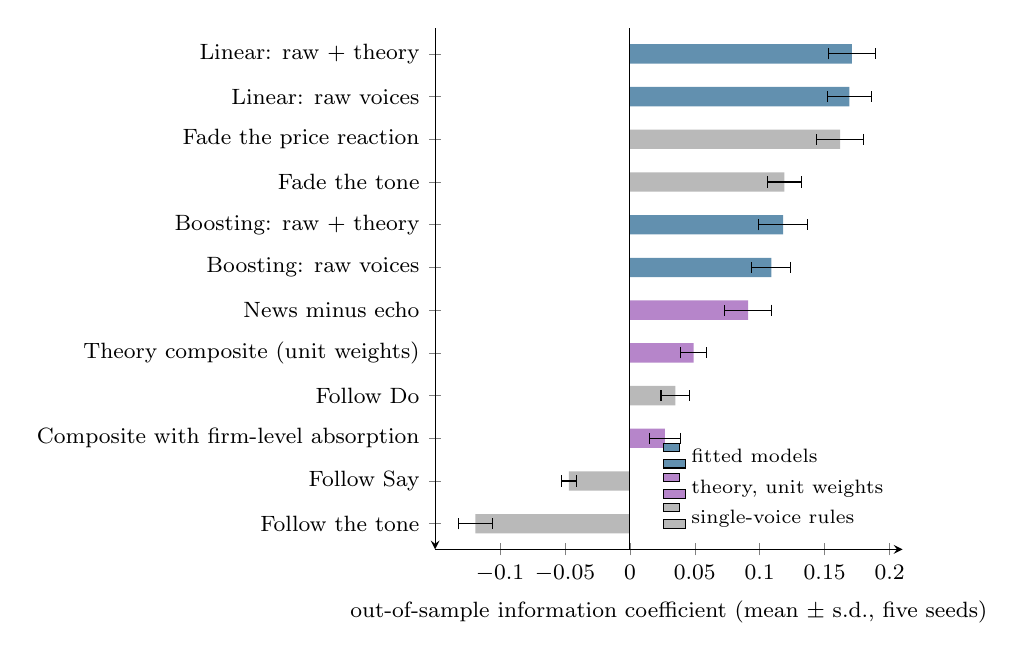
\begin{tikzpicture}
\begin{axis}[xbar, width=0.62\textwidth, height=8.2cm, bar width=7pt,
  xmin=-0.15, xmax=0.21, ymin=0.4, ymax=12.6, y dir=reverse,
  ytick={1,...,12},
  yticklabels={Linear: raw + theory, Linear: raw voices, Fade the price reaction, Fade the tone, Boosting: raw + theory, Boosting: raw voices, News minus echo, Theory composite (unit weights), Follow Do, Composite with firm-level absorption, Follow Say, Follow the tone},
  xtick={-0.1,-0.05,0,0.05,0.1,0.15,0.2},
  xticklabel style={/pgf/number format/fixed, /pgf/number format/precision=2},
  xlabel={\footnotesize out-of-sample information coefficient (mean $\pm$ s.d., five seeds)},
  tick label style={font=\footnotesize}, axis lines=left,
  legend style={font=\scriptsize, draw=none, fill=none, at={(0.99,0.02)}, anchor=south east}, legend cell align=left]
\addplot[fill=do!70, draw=none, bar shift=0pt, error bars/.cd, x dir=both, x explicit]
  coordinates {(0.171,1) +- (0.018,0) (0.169,2) +- (0.017,0) (0.118,5) +- (0.019,0) (0.109,6) +- (0.015,0)};
\addlegendentry{fitted models}
\addplot[fill=say!65, draw=none, bar shift=0pt, error bars/.cd, x dir=both, x explicit]
  coordinates {(0.091,7) +- (0.018,0) (0.049,8) +- (0.010,0) (0.027,10) +- (0.012,0)};
\addlegendentry{theory, unit weights}
\addplot[fill=gray!55, draw=none, bar shift=0pt, error bars/.cd, x dir=both, x explicit]
  coordinates {(0.162,3) +- (0.018,0) (0.119,4) +- (0.013,0) (0.035,9) +- (0.011,0) (-0.047,11) +- (0.006,0) (-0.119,12) +- (0.013,0)};
\addlegendentry{single-voice rules}
\draw[black] (axis cs:0,0.4) -- (axis cs:0,12.6);
\end{axis}
\end{tikzpicture}
\caption{Out-of-sample forecasts in the main simulated market. The fitted models use the training half. ``Raw voices'' are Say, Do, tone, article count and the price reaction; ``theory'' adds the features of \cref{tab:features}.}
\label{fig:ic}
\end{figure}

\paragraph{Robustness.} \Cref{tab:robust} changes one assumption at a time on three new seeds. Fat-tailed values and power-law echo delays (a misspecified kernel) leave the echo, news and detection results intact. Partial disclosure, in which only $30\%$ of the trade is disclosed and positioning is measured with twice the noise, leaves the echo and news results intact but lowers the detection AUC to $0.857$. A saturating crowd, which prices $1.5\tanh(s/1.5)$ instead of $s$, halves the IC of every forecast, but detection is unaffected and the echo and news signs survive. The controlled test of reversed words (\cref{tab:tests}, fourth row) does not: under the saturating crowd its $t$-statistic has the wrong sign in all three seeds. When meaning is weak ($\varkappa=5$) or ignored, the echo share is underestimated by about six percentage points and the echo test weakens, as \cref{thm:semantic} leads one to expect. More events per firm strengthen the echo test, somewhat more slowly than the square root of the sample: over two seeds the $t$-statistic is $-5.4$, $-6.9$ and $-9.3$ with $20$, $40$ and $80$ events, while detection stays at an AUC of $0.93$--$0.94$.

\begin{table}[ht]
\centering
\caption{Robustness: one change at a time, three seeds each. ``Reference'' is the main market on the same seeds. IC: out-of-sample information coefficient. Echo share: estimated (true).}
\label{tab:robust}
\small
\setlength{\tabcolsep}{3.6pt}
\begin{tabular}{@{}lrrrrrrrc@{}}
\toprule
& \multicolumn{3}{c}{IC} & \multicolumn{3}{c}{$t$-statistic} & & \\
\cmidrule(lr){2-4}\cmidrule(lr){5-7}
Variant & fade price & linear & + theory & echo & news & L\'evy & AUC & echo share \\
\midrule
Reference & $0.184$ & $0.187$ & $0.190$ & $-7.5$ & $+3.6$ & $+3.6$ & $0.941$ & $0.425$ ($0.430$) \\
Fat tails ($t_3$ values) & $0.134$ & $0.137$ & $0.141$ & $-8.1$ & $+2.4$ & $+0.5$ & $0.924$ & $0.423$ ($0.428$) \\
Saturating crowd & $0.090$ & $0.099$ & $0.101$ & $-5.9$ & $+3.2$ & $-0.0$ & $0.942$ & $0.425$ ($0.430$) \\
Power-law echo delays & $0.171$ & $0.176$ & $0.177$ & $-7.9$ & $+2.1$ & $+1.9$ & $0.939$ & $0.417$ ($0.429$) \\
30\% of trade disclosed & $0.184$ & $0.183$ & $0.191$ & $-7.5$ & $+4.1$ & $+2.9$ & $0.857$ & $0.425$ ($0.430$) \\
Weak meaning ($\varkappa=5$) & $0.173$ & $0.187$ & $0.188$ & $-7.2$ & $+1.9$ & $+2.2$ & $0.941$ & $0.373$ ($0.429$) \\
Timing only (reference markets) & $0.184$ & $0.187$ & $0.189$ & $-6.0$ & $+2.6$ & $+3.7$ & $0.940$ & $0.368$ ($0.430$) \\
\bottomrule
\end{tabular}
\end{table}

\paragraph{Q5: return-aligned embeddings organise text by consequence.} For the embedding results we generated a corpus of short synthetic headlines. Each headline mixes four topic words, two tone words, one cue that decides whether the move is \emph{overdone} (it reverses within a week) or \emph{fundamental} (it continues), three filler words and a company code. Topic words are numerous and have nothing to do with outcomes, so a generic bag-of-words geometry groups headlines by topic. Each headline has a three-part outcome: the next-day move, the week-ahead move and the change in implied volatility. We trained a $16$-dimensional linear projection of TF-IDF vectors with the loss of \cref{thm:racl} ($\tau=0.1$, bandwidth by the median heuristic, $600$ Adam steps on batches of $256$) on $2{,}000$ headlines, and tested it on $1{,}000$ new ones.

Training moves the geometry from topic to consequence (\cref{tab:text,fig:text}a). In TF-IDF space the ten nearest neighbours of a test headline share its topic $85\%$ of the time and its consequence (tone and cue together) $51\%$ of the time. After training they share its consequence $100\%$ of the time and its topic $34\%$ of the time, close to the chance level of $25\%$. The analog forecast of \cref{prop:analog} predicts the week-ahead move with an IC of $0.892$, against $0.192$ for TF-IDF neighbours and a ceiling of $0.936$ set by the outcome noise. Linear regression on the same words fails completely ($-0.02$), because the outcome depends on the \emph{interaction} of tone and cue, which a linear model of word counts cannot express. Gradient boosting captures the interaction ($0.837$) but falls short of the embedding. That comparison favours the embedding, which is trained on all three outcomes: the next-day move reveals the tone and the volatility change reveals the cue, while boosting sees only the week-ahead target.

The certificate is the negative result (\cref{fig:text}b). After training, the mean excess loss per anchor is $0.021$--$0.026$ across seeds. That is small, but target probabilities over $149$ neighbours are of order $1/149\approx0.007$, and neither form of \cref{thm:robustnn} certifies a single comparison. Two things stand in the way. The median-heuristic bandwidth makes the targets almost flat, and the part of each outcome that the text cannot predict leaves an excess loss that no embedding can remove. When we remove both obstacles, using noise-free outcomes and a bandwidth of $0.3$ times the median, the exact form (ii) certifies $45\%$ of the ordered comparisons with no errors, while the Pinsker form (i) still certifies none. With the sharp bandwidth and realistic outcome noise, the excess loss stays at $0.14$ and nothing is certified, even though the analog IC rises to $0.931$, close to its ceiling. The certificate never made a wrong claim in any run. It becomes informative, however, only when outcomes are close to predictable from the text, which real returns are not.

\begin{table}[ht]
\centering
\caption{Text experiment: $1{,}000$ test headlines, mean $\pm$ s.d.\ over three seeds. Neighbour columns: share of the ten nearest training headlines with the same consequence (tone and cue) or the same topic; chance is $0.25$ for both. The ceiling for the IC is $0.936$.}
\label{tab:text}
\small
\begin{tabular}{@{}lrrr@{}}
\toprule
Method & Week-ahead IC & Same consequence & Same topic \\
\midrule
TF-IDF neighbours (generic) & $0.192\pm0.003$ & $0.506$ & $0.846$ \\
Random 16-d projection (generic) & $0.039\pm0.016$ & $0.327$ & $0.622$ \\
Ridge regression on words (supervised) & $-0.019\pm0.016$ & -- & -- \\
Gradient boosting on words (supervised) & $0.837\pm0.008$ & -- & -- \\
Return-aligned embedding, 16-d & $\mathbf{0.892\pm0.009}$ & $\mathbf{1.000}$ & $0.344$ \\
\bottomrule
\end{tabular}
\end{table}

\begin{figure}[ht]
\centering
\begin{minipage}[t]{0.48\textwidth}
\centering
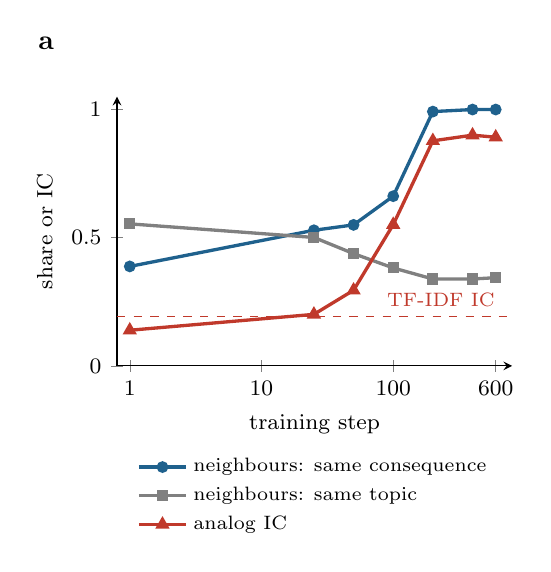
\begin{tikzpicture}
\begin{semilogxaxis}[width=6.6cm, height=5.0cm, xmin=0.8, xmax=800, ymin=0, ymax=1.05,
  xtick={1,10,100,600}, xticklabels={1,10,100,600},
  xlabel={\footnotesize training step}, ylabel={\footnotesize share or IC},
  tick label style={font=\footnotesize}, axis lines=left,
  legend style={font=\scriptsize, draw=none, fill=none, at={(0.5,-0.30)}, anchor=north}, legend cell align=left]
\addplot[do, very thick, mark=*, mark size=1.5pt] coordinates {(1,0.388) (25,0.529) (50,0.550) (100,0.662) (200,0.992) (400,1.000) (600,1.000)};
\addlegendentry{neighbours: same consequence}
\addplot[gray, very thick, mark=square*, mark size=1.4pt] coordinates {(1,0.554) (25,0.501) (50,0.438) (100,0.382) (200,0.339) (400,0.339) (600,0.344)};
\addlegendentry{neighbours: same topic}
\addplot[echo, very thick, mark=triangle*, mark size=1.8pt] coordinates {(1,0.139) (25,0.201) (50,0.295) (100,0.551) (200,0.878) (400,0.900) (600,0.892)};
\addlegendentry{analog IC}
\addplot[echo, dashed, domain=0.8:800, samples=2] {0.192};
\node[font=\scriptsize, text=echo, anchor=south east] at (axis cs:700,0.192) {TF-IDF IC};
\end{semilogxaxis}
\node[font=\bfseries] at (-0.9,4.1) {a};
\end{tikzpicture}
\end{minipage}\hfill
\begin{minipage}[t]{0.48\textwidth}
\centering
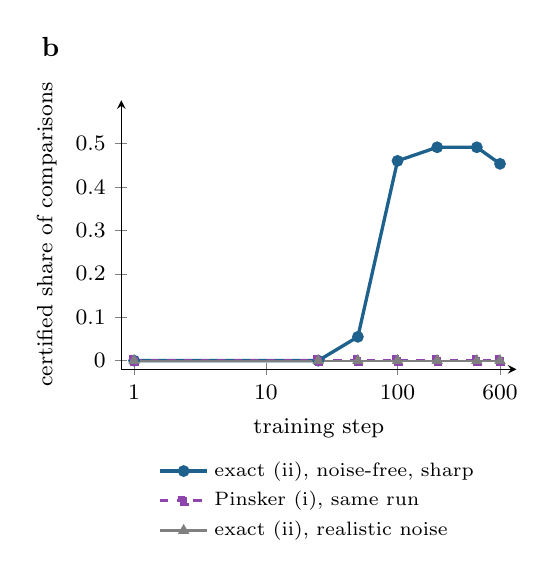
\begin{tikzpicture}
\begin{semilogxaxis}[width=6.6cm, height=5.0cm, xmin=0.8, xmax=800, ymin=-0.02, ymax=0.6,
  xtick={1,10,100,600}, xticklabels={1,10,100,600},
  ytick={0,0.1,0.2,0.3,0.4,0.5},
  yticklabel style={/pgf/number format/fixed, /pgf/number format/precision=1},
  xlabel={\footnotesize training step}, ylabel={\footnotesize certified share of comparisons},
  tick label style={font=\footnotesize}, axis lines=left,
  legend style={font=\scriptsize, draw=none, fill=none, at={(0.5,-0.30)}, anchor=north}, legend cell align=left]
\addplot[do, very thick, mark=*, mark size=1.5pt] coordinates {(1,0) (25,0) (50,0.0549) (100,0.4602) (200,0.4915) (400,0.4915) (600,0.4534)};
\addlegendentry{exact (ii), noise-free, sharp}
\addplot[say, very thick, dashed, mark=square*, mark size=1.3pt] coordinates {(1,0) (25,0) (50,0) (100,0) (200,0) (400,0) (600,0)};
\addlegendentry{Pinsker (i), same run}
\addplot[gray, thick, mark=triangle*, mark size=1.6pt, mark options={solid}] coordinates {(1,0) (25,0) (50,0) (100,0) (200,0) (400,0) (600,0)};
\addlegendentry{exact (ii), realistic noise}
\end{semilogxaxis}
\node[font=\bfseries] at (-0.9,4.1) {b};
\end{tikzpicture}
\end{minipage}
\caption{Return-aligned training. \textbf{a}: the ten nearest neighbours of test headlines switch from sharing a topic to sharing a consequence, and the analog forecast improves with them (mean of three seeds). \textbf{b}: share of ordered outcome comparisons certified by \cref{thm:robustnn} on $150$ training anchors. With noise-free outcomes and a bandwidth of $0.3$ times the median, the exact form certifies about half of them. The Pinsker form certifies none, and with realistic outcome noise neither form certifies any. No certified comparison was ever wrong.}
\label{fig:text}
\end{figure}


\begin{tcolorbox}[enhanced,breakable,colback=gray!4,colframe=gray!55!black,boxrule=0.6pt,arc=2pt,
  fonttitle=\bfseries\small,title={What the experiments show, and what they do not},left=8pt,right=8pt]
\small
\textbf{Supported.} Echoes can be separated from news, and meaning helps. Fading the echo works in every market we simulated, and following the news works in most. The rolling Say--Do covariance identifies the institutions whose words should be faded. It flags false-alarm events with an AUC of $0.90$ on its own and $0.93$ in a supervised detector. Return-aligned training organises text by consequence rather than topic.

\textbf{Only partly supported.} The lead--lag signal has the right sign but is weak. The flagged group's reversed words are significant only when echoes are not controlled, and the controlled version fails under a saturating crowd. The theory's features help flexible learners a little and a linear model almost not at all, but the simulation leaves little room for any method to improve.

\textbf{Not supported here.} Estimated absorption reversed everywhere because the narrative model it relies on was too crude. With the exact narrative move, its coefficient is near zero, so the experiments do not test \cref{thm:absorption}. The unit-weight composite is not a good trading rule. With realistic outcome noise, the neighbour certificate certified no comparison. Its exact form does certify about half of all comparisons when outcomes are noise-free and targets are sharp, a case in which the Pinsker form certifies none.

\textbf{Not tested.} Everything above is simulated, and the simulator shares the theory's structure. Only market data can say whether real institutions behave like the ones in \cref{sec:strategic}.
\end{tcolorbox}

% =====================================================================
\section{Discussion}\label{sec:discussion}

\paragraph{Scope of the theory.} The price-formation results are exact in a linear--Gaussian economy with reduced-form crowd pricing. They pin down \emph{signs} and \emph{sufficient statistics}, not magnitudes. The embedding, Hawkes, signature, detection, conformal and Kelly results are model-agnostic within their stated assumptions.

\paragraph{What the experiments add.} The controlled experiments of \cref{sec:experiments} separate the parts of the framework that are ready for data from the parts that are not. The echo decomposition and Say--Do detection held under every variation we tried. The reversed-words regression was less robust. Absorption needs a better model of the narrative-implied move before its sign can be trusted: at a minimum, cascade size should enter multiplicatively, and the sign should be estimated in each market. The neighbour certificate needs outcome targets smoother than raw returns, for example targets averaged over similar past events, before it can certify anything. These are the first things we would change before running the test on real data.

\paragraph{Empirical programme.} The theory yields sharp, falsifiable predictions: opposite signs on $s^{\text{new}}$ and $s^{\text{echo}}$; a positive loading on $-G_\gamma$; an absorption loading whose sign flips with the informed-to-noise ratio of \cref{thm:absorption}, which can be proxied by flow toxicity or liquidity; higher returns after positive L\'evy area; a negative Say--Do covariance in episodes that are later classified as manipulative; false alarms concentrated at intermediate echo shares in liquid markets; and negative autocorrelation of the rolling Say--Do covariance where impact and misreporting costs are moderate. The controlled experiments suggest the order of the tests: the echo prediction and Say--Do detection first, since they were the most robust, and absorption last. Testing requires point-in-time data, purged combinatorial cross-validation, deflated performance statistics and controls for look-ahead in pretrained language models \citep{lopezdeprado2018,bailey2014dsr,glasserman2023}. We leave this to companion work.

\paragraph{Limitations.} Crowd pricing is reduced-form (in \cref{sec:strategic} the crowd's credulity is exogenous within a round and adaptive across rounds); \cref{thm:levy} assumes smooth, stationary paths; and \cref{thm:detect} assumes i.i.d.\ emissions within an episode. The simulator of \cref{sec:experiments} shares the theory's structure and is far more predictable than any real market, so its results show that the tools can work, not that they will. Each assumption marks a direction for extension.

\paragraph{Ethics and compliance.} A strategic reading means that narrative and capital moved in opposite directions in a particular order. It is not evidence of deception, and firms maintain information barriers between research and trading. The framework uses public information and lawful disclosures only; it must never be used to create or disseminate narratives intended to move prices.

\paragraph{Code availability.} A tested Python implementation of every result in this paper is available at \url{https://github.com/AliAtiah/say-echo-do}. It includes scripts that regenerate \cref{tab:verify}, the quantitative figures, and every experiment of \cref{sec:experiments}.

% =====================================================================
\appendix
\section{Auxiliary Lemmas}\label{app:aux}

\begin{lemma}[Gaussian conditioning]\label{lem:gauss}
If $(\bm a,\bm b)$ is jointly Gaussian with $\Var(\bm b)\succ0$, then $\E[\bm a\mid\bm b]=\E\bm a+\Cov(\bm a,\bm b)\Var(\bm b)^{-1}(\bm b-\E\bm b)$ and $\Var(\bm a\mid\bm b)=\Var(\bm a)-\Cov(\bm a,\bm b)\Var(\bm b)^{-1}\Cov(\bm b,\bm a)$. The same formulas hold conditionally on a further jointly Gaussian vector.
\end{lemma}
\begin{proof}
Let $\bm e=\bm a-\E\bm a-\Cov(\bm a,\bm b)\Var(\bm b)^{-1}(\bm b-\E\bm b)$. Then $\Cov(\bm e,\bm b)=0$, and joint Gaussianity makes $\bm e$ independent of $\bm b$. Hence $\E[\bm a\mid\bm b]$ is as stated, and $\Var(\bm a\mid\bm b)=\Var(\bm e)$, which expands to the stated formula.
\end{proof}

\begin{lemma}[Bhattacharyya coefficient of Gaussians]\label{lem:bc}
For $p_i=\N(\bm m_i,\Sigma)$ on $\R^d$, $\int\sqrt{p_0p_1}=\exp\big(-\tfrac18(\bm m_1-\bm m_0)^\top\Sigma^{-1}(\bm m_1-\bm m_0)\big)$.
\end{lemma}
\begin{proof}
With $\bar{\bm m}=(\bm m_0+\bm m_1)/2$ and $\bm\delta=\bm m_1-\bm m_0$, the identity $\tfrac12(\bm x-\bm m_0)^\top\Sigma^{-1}(\bm x-\bm m_0)+\tfrac12(\bm x-\bm m_1)^\top\Sigma^{-1}(\bm x-\bm m_1)=(\bm x-\bar{\bm m})^\top\Sigma^{-1}(\bm x-\bar{\bm m})+\tfrac14\bm\delta^\top\Sigma^{-1}\bm\delta$ gives $\sqrt{p_0p_1}=\N(\bm x;\bar{\bm m},\Sigma)\,e^{-\bm\delta^\top\Sigma^{-1}\bm\delta/8}$. Integrate over $\bm x$.
\end{proof}

\section{Implementation Notes}\label{app:impl}

\paragraph{Encoder.} A transformer sentence encoder \citep{reimers2019} with mean pooling and $\ell_2$ normalisation, adapted with low-rank adapters, trained on $\mathcal{L}+\mu_a\,\KL$-anchor with $\tau=0.05$ and bandwidth $b$ by the median heuristic, on rolling windows whose outcome horizons close before each refit date.

\paragraph{Surprise model.} A causal transformer over the last 32 article embeddings and the market state, with Gaussian predictive head and Ledoit--Wolf shrinkage of $\Sigma$ \citep{ledoit2004}.

\paragraph{Hawkes.} Exponential kernels fitted by maximum likelihood per semantic cluster on trailing windows. The parentage probabilities of \cref{prop:parentage} are computed in $O(N)$ with the exponential recursion for $\lambda(\tau_j)$.

\paragraph{Positioning.} A lag-augmented Kalman filter merges disclosures released at different frequencies and delays, and its posterior variance supplies $\sigma_x^2$ in \cref{thm:saydo}.

\paragraph{L\'evy area.} Computed on piecewise-linear interpolations of standardised positioning and gloom with \cref{prop:levyprops}(v), over rolling windows.

% =====================================================================
\clearpage
\begin{thebibliography}{99}\small

\bibitem[Araci(2019)]{araci2019} Araci, D. (2019). FinBERT: Financial sentiment analysis with pre-trained language models. arXiv:1908.10063.
\bibitem[Bacry et al.(2015)]{bacry2015} Bacry, E., Mastromatteo, I., and Muzy, J.-F. (2015). Hawkes processes in finance. \emph{Market Microstructure and Liquidity}, 1(1), 1550005.
\bibitem[Bailey and L\'opez de Prado(2014)]{bailey2014dsr} Bailey, D.~H., and L\'opez de Prado, M. (2014). The deflated Sharpe ratio: Correcting for selection bias, backtest overfitting, and non-normality. \emph{Journal of Portfolio Management}, 40(5), 94--107.
\bibitem[Baker and Wurgler(2006)]{baker2006} Baker, M., and Wurgler, J. (2006). Investor sentiment and the cross-section of stock returns. \emph{Journal of Finance}, 61(4), 1645--1680.
\bibitem[Barber and Odean(2008)]{barber2008} Barber, B.~M., and Odean, T. (2008). All that glitters: The effect of attention and news on the buying behavior of individual and institutional investors. \emph{Review of Financial Studies}, 21(2), 785--818.
\bibitem[Bhattacharyya(1943)]{bhattacharyya1943} Bhattacharyya, A. (1943). On a measure of divergence between two statistical populations defined by their probability distributions. \emph{Bulletin of the Calcutta Mathematical Society}, 35, 99--109.
\bibitem[Blackwell(1953)]{blackwell1953} Blackwell, D. (1953). Equivalent comparisons of experiments. \emph{Annals of Mathematical Statistics}, 24(2), 265--272.
\bibitem[Bouchaud et al.(2018)]{bouchaud2018} Bouchaud, J.-P., Bonart, J., Donier, J., and Gould, M. (2018). \emph{Trades, Quotes and Prices: Financial Markets Under the Microscope}. Cambridge University Press.
\bibitem[Brunnermeier and Pedersen(2005)]{brunnermeier2005} Brunnermeier, M.~K., and Pedersen, L.~H. (2005). Predatory trading. \emph{Journal of Finance}, 60(4), 1825--1863.
\bibitem[Chan(2003)]{chan2003} Chan, W.~S. (2003). Stock price reaction to news and no-news: Drift and reversal after headlines. \emph{Journal of Financial Economics}, 70(2), 223--260.
\bibitem[Chevyrev and Kormilitzin(2016)]{chevyrev2016} Chevyrev, I., and Kormilitzin, A. (2016). A primer on the signature method in machine learning. arXiv:1603.03788.
\bibitem[Cohen et al.(2012)]{cohen2012} Cohen, L., Malloy, C., and Pomorski, L. (2012). Decoding inside information. \emph{Journal of Finance}, 67(3), 1009--1043.
\bibitem[Cont et al.(2014)]{cont2014} Cont, R., Kukanov, A., and Stoikov, S. (2014). The price impact of order book events. \emph{Journal of Financial Econometrics}, 12(1), 47--88.
\bibitem[Da et al.(2011)]{da2011} Da, Z., Engelberg, J., and Gao, P. (2011). In search of attention. \emph{Journal of Finance}, 66(5), 1461--1499.
\bibitem[De Long et al.(1990)]{delong1990} De Long, J.~B., Shleifer, A., Summers, L.~H., and Waldmann, R.~J. (1990). Noise trader risk in financial markets. \emph{Journal of Political Economy}, 98(4), 703--738.
\bibitem[Engelberg et al.(2012)]{engelberg2012} Engelberg, J.~E., Reed, A.~V., and Ringgenberg, M.~C. (2012). How are shorts informed? Short sellers, news, and information processing. \emph{Journal of Financial Economics}, 105(2), 260--278.
\bibitem[Gibbs and Cand\`es(2021)]{gibbs2021} Gibbs, I., and Cand\`es, E. (2021). Adaptive conformal inference under distribution shift. \emph{Advances in Neural Information Processing Systems}, 34.
\bibitem[Glasserman and Lin(2023)]{glasserman2023} Glasserman, P., and Lin, C. (2023). Assessing look-ahead bias in stock return predictions generated by GPT sentiment analysis. arXiv:2309.17322.
\bibitem[Glosten and Milgrom(1985)]{glosten1985} Glosten, L.~R., and Milgrom, P.~R. (1985). Bid, ask and transaction prices in a specialist market with heterogeneously informed traders. \emph{Journal of Financial Economics}, 14(1), 71--100.
\bibitem[Hawkes(1971)]{hawkes1971} Hawkes, A.~G. (1971). Spectra of some self-exciting and mutually exciting point processes. \emph{Biometrika}, 58(1), 83--90.
\bibitem[Hawkes and Oakes(1974)]{hawkesoakes1974} Hawkes, A.~G., and Oakes, D. (1974). A cluster process representation of a self-exciting process. \emph{Journal of Applied Probability}, 11(3), 493--503.
\bibitem[Hong and Stein(1999)]{hong1999} Hong, H., and Stein, J.~C. (1999). A unified theory of underreaction, momentum trading, and overreaction in asset markets. \emph{Journal of Finance}, 54(6), 2143--2184.
\bibitem[Kailath(1967)]{kailath1967} Kailath, T. (1967). The divergence and Bhattacharyya distance measures in signal selection. \emph{IEEE Transactions on Communication Technology}, 15(1), 52--60.
\bibitem[Ke et al.(2019)]{ke2019} Ke, Z.~T., Kelly, B.~T., and Xiu, D. (2019). Predicting returns with text data. NBER Working Paper 26186.
\bibitem[Kelly(1956)]{kelly1956} Kelly, J.~L. (1956). A new interpretation of information rate. \emph{Bell System Technical Journal}, 35(4), 917--926.
\bibitem[Kogan et al.(2023)]{kogan2023} Kogan, S., Moskowitz, T.~J., and Niessner, M. (2023). Social media and financial news manipulation. \emph{Review of Finance}, 27(4), 1229--1268.
\bibitem[Kyle(1985)]{kyle1985} Kyle, A.~S. (1985). Continuous auctions and insider trading. \emph{Econometrica}, 53(6), 1315--1335.
\bibitem[Ledoit and Wolf(2004)]{ledoit2004} Ledoit, O., and Wolf, M. (2004). A well-conditioned estimator for large-dimensional covariance matrices. \emph{Journal of Multivariate Analysis}, 88(2), 365--411.
\bibitem[L\'evy(1940)]{levy1940} L\'evy, P. (1940). Le mouvement brownien plan. \emph{American Journal of Mathematics}, 62(1), 487--550.
\bibitem[L\'opez de Prado(2018)]{lopezdeprado2018} L\'opez de Prado, M. (2018). \emph{Advances in Financial Machine Learning}. Wiley.
\bibitem[Lopez-Lira and Tang(2023)]{lopezlira2023} Lopez-Lira, A., and Tang, Y. (2023). Can ChatGPT forecast stock price movements? Return predictability and large language models. arXiv:2304.07619.
\bibitem[Loughran and McDonald(2011)]{loughran2011} Loughran, T., and McDonald, B. (2011). When is a liability not a liability? Textual analysis, dictionaries, and 10-Ks. \emph{Journal of Finance}, 66(1), 35--65.
\bibitem[Lyons(1998)]{lyons1998} Lyons, T.~J. (1998). Differential equations driven by rough signals. \emph{Revista Matem\'atica Iberoamericana}, 14(2), 215--310.
\bibitem[Merton(1969)]{merton1969} Merton, R.~C. (1969). Lifetime portfolio selection under uncertainty: The continuous-time case. \emph{Review of Economics and Statistics}, 51(3), 247--257.
\bibitem[van den Oord et al.(2018)]{oord2018} van den Oord, A., Li, Y., and Vinyals, O. (2018). Representation learning with contrastive predictive coding. arXiv:1807.03748.
\bibitem[Park et al.(2023)]{park2023} Park, K., Choe, Y.~J., and Veitch, V. (2023). The linear representation hypothesis and the geometry of large language models. arXiv:2311.03658.
\bibitem[Reimers and Gurevych(2019)]{reimers2019} Reimers, N., and Gurevych, I. (2019). Sentence-BERT: Sentence embeddings using Siamese BERT-networks. \emph{Proceedings of EMNLP-IJCNLP}.
\bibitem[Shiller(2017)]{shiller2017} Shiller, R.~J. (2017). Narrative economics. \emph{American Economic Review}, 107(4), 967--1004.
\bibitem[Shleifer and Vishny(1997)]{shleifer1997} Shleifer, A., and Vishny, R.~W. (1997). The limits of arbitrage. \emph{Journal of Finance}, 52(1), 35--55.
\bibitem[Tetlock(2007)]{tetlock2007} Tetlock, P.~C. (2007). Giving content to investor sentiment: The role of media in the stock market. \emph{Journal of Finance}, 62(3), 1139--1168.
\bibitem[Veronesi(1999)]{veronesi1999} Veronesi, P. (1999). Stock market overreaction to bad news in good times: A rational expectations equilibrium model. \emph{Review of Financial Studies}, 12(5), 975--1007.
\bibitem[Zhuang et al.(2002)]{zhuang2002} Zhuang, J., Ogata, Y., and Vere-Jones, D. (2002). Stochastic declustering of space-time earthquake occurrences. \emph{Journal of the American Statistical Association}, 97(458), 369--380.

\bibitem[B\'enabou and Laroque(1992)]{benabou1992} B\'enabou, R., and Laroque, G. (1992). Using privileged information to manipulate markets: Insiders, gurus, and credibility. \emph{Quarterly Journal of Economics}, 107(3), 921--958.
\bibitem[Crawford and Sobel(1982)]{crawford1982} Crawford, V.~P., and Sobel, J. (1982). Strategic information transmission. \emph{Econometrica}, 50(6), 1431--1451.
\bibitem[Evans and Honkapohja(2001)]{evans2001} Evans, G.~W., and Honkapohja, S. (2001). \emph{Learning and Expectations in Macroeconomics}. Princeton University Press.
\bibitem[Ezekiel(1938)]{ezekiel1938} Ezekiel, M. (1938). The cobweb theorem. \emph{Quarterly Journal of Economics}, 52(2), 255--280.
\bibitem[Kartik et al.(2007)]{kartik2007} Kartik, N., Ottaviani, M., and Squintani, F. (2007). Credulity, lies, and costly talk. \emph{Journal of Economic Theory}, 134(1), 93--116.
\bibitem[Llorente et al.(2002)]{llorente2002} Llorente, G., Michaely, R., Saar, G., and Wang, J. (2002). Dynamic volume-return relation of individual stocks. \emph{Review of Financial Studies}, 15(4), 1005--1047.
\bibitem[May(1976)]{may1976} May, R.~M. (1976). Simple mathematical models with very complicated dynamics. \emph{Nature}, 261, 459--467.
\bibitem[van Bommel(2003)]{vanbommel2003} van Bommel, J. (2003). Rumors. \emph{Journal of Finance}, 58(4), 1499--1520.
\end{thebibliography}

\end{document}
